% Possible types of documents/theses
%   doctype=bachelorsthesis
%   doctype=mastersthesis
%   doctype=idp
%   doctype=phdthesis
%   doctype=studienarbeit
%   doctype=diplomarbeit
%
% Document language
%   without 'lang' attribute: English
%   lang=ngerman:             German (new orthography)
%
% Binding correction
%   BCOR=<Längenangabe>
%   Additional margin, which is invisible due to binding the book
%   The usual binding by the Fachschaft has a thickness of 1,5 cm 
%
% biblatex (citations)
%   This requires 'biber' to be used instead of 'bibtex', please
%   adapt your editor's settings accordingly!
\documentclass[doctype=mastersthesis,BCOR=15mm,biblatex]{ldvbook}%lang=ngerman

% !TeX spellcheck = en_US

\usepackage{placeins}

\usepackage{pgfplots}
\usepackage{tikz}
\usetikzlibrary{calc}
\usetikzlibrary{matrix}
\usetikzlibrary{ decorations.markings}
\usetikzlibrary {decorations.shapes}

\usepackage{xcolor}

\definecolor{C0}{HTML}{1f77b4}
\definecolor{C1}{HTML}{ff7f0e}
\definecolor{C2}{HTML}{2ca02c}
\definecolor{C3}{HTML}{d62728}
\definecolor{C4}{HTML}{9467bd}
\definecolor{C5}{HTML}{8c564b}
\definecolor{C6}{HTML}{e377c2}
\definecolor{C7}{HTML}{7f7f7f}
\definecolor{C8}{HTML}{bcbd22}
\definecolor{C9}{HTML}{17becf}

\tikzstyle{colmarking} = [C0,line width=1.5pt]
\def\colortext{C0}

\usetikzlibrary{calc}
\usetikzlibrary{matrix}
\usetikzlibrary{ decorations.markings}
\usetikzlibrary {decorations.shapes}


%Standard settings for the stage4s
\tikzset{
	style_stage/.style={
		color=black!80, %line color
		draw,
		fill=white,
		line width=1pt,
	}
}

%special parametres for stages
\tikzset{fontmatrices/.initial=\small}
\tikzset{boxsize/.initial=9mm} %Note: width=height=2*boxsize
%psoition of arrow
\tikzset{posarr/.initial=0.5}

%line style for the signals
\tikzstyle{signal} = [line width=1.5pt]%[very thick]

%line style for drawing connections
\tikzset{signalflow/.style={signal,
		decoration={markings,mark=at position \pgfkeysvalueof{/tikz/posarr} with {\arrow{>}}},postaction={decorate}}}

%set the standard parameters for A,B,C,D
\tikzset{A/.initial=$A_{}$}
\tikzset{B/.initial=$B_{}$}
\tikzset{C/.initial=$C_{}$}
\tikzset{D/.initial=$D_{}$}


%Some internal definitions
\def\rel_i_stage{0.65} %distance of the connections for B and C, is a fraction of boxsize
\def\shadesize{2pt}

%some shorthanfds for convenience
\def\boxsize{\pgfkeysvalueof{/tikz/boxsize}}

\makeatletter
\pgfdeclareshape{stagebox}{
	%anchors
	\anchor{center}{\pgf@x=0cm \pgf@y=0cm}
	\anchor{south}{\pgf@x=0cm \pgf@y=-\boxsize}
	\anchor{east}{\pgf@x=\boxsize \pgf@y=0cm}
	\anchor{west}{\pgf@x=-\boxsize \pgf@y=0cm}
	\anchor{north}{\pgf@x=0cm \pgf@y=\boxsize}

	%draw
	\backgroundpath{
		\filldraw(-\boxsize,-\boxsize)rectangle(\boxsize,\boxsize);
    }
}
\makeatother

\makeatletter
\pgfdeclareshape{stage}{
	%anchors
	\anchor{center}{\pgf@x=0cm \pgf@y=0cm}
	\anchor{south}{\pgf@x=0cm \pgf@y=-\boxsize}
	\anchor{east}{\pgf@x=\boxsize \pgf@y=0cm}
	\anchor{west}{\pgf@x=-\boxsize \pgf@y=0cm}
	\anchor{north}{\pgf@x=0cm \pgf@y=\boxsize}

	\anchor{xout}{\pgf@x=0cm \pgf@y=-\boxsize}
	\anchor{y}{\pgf@x=\boxsize \pgf@y=0cm}
	\anchor{u}{\pgf@x=-\boxsize \pgf@y=0cm}
	\anchor{xin}{\pgf@x=0cm \pgf@y=\boxsize}

	%draw
	\backgroundpath{
		\filldraw(-\boxsize,-\boxsize)rectangle(\boxsize,\boxsize);

		%connection A
		\draw[signal][postaction = {decorate,decoration={markings,mark= at position 0.65 with {\arrow{>}}}}]
					(-\boxsize,0) -- (\boxsize,0);
		%shade at the intersection
		\filldraw[draw=none,opacity=0.7](-\shadesize,-\shadesize)rectangle(\shadesize,\shadesize);
		%connection D
		\draw[signal][postaction = {decorate,decoration={markings,mark= at position 0.35 with {\arrow{>}}}}]
					(0,\boxsize) -- (0,-\boxsize);



		%connections for B and C
		\draw[signal][postaction = {decorate,decoration={markings,mark= at position 0.6 with {\arrow{>}}}}]
					(-\rel_i_stage*\boxsize,0) -- (0,-\rel_i_stage*\boxsize);
		\draw[signal][postaction = {decorate,decoration={markings,mark= at position 0.6 with {\arrow{>}}}}]
					(0,\rel_i_stage*\boxsize) -- (\rel_i_stage*\boxsize,0);

		%Text for A,B,D,C
		\pgfsetcolor{black}
		\pgftext[right,x=-0.5em,y=0.4*\boxsize]
			{\pgfkeysvalueof{/tikz/fontmatrices} \pgfkeysvalueof{/tikz/A}}
		\pgftext[top,left,x=0.05*\boxsize,y=-0.5em]
			{\pgfkeysvalueof{/tikz/fontmatrices} \pgfkeysvalueof{/tikz/D}}
		\pgftext[left,bottom,x=0.35*\boxsize,y=0.35*\boxsize]
			{\pgfkeysvalueof{/tikz/fontmatrices} \pgfkeysvalueof{/tikz/C}}
		\pgftext[right,top,x=-0.35*\boxsize,y=-0.4*\boxsize]
			{\pgfkeysvalueof{/tikz/fontmatrices} \pgfkeysvalueof{/tikz/B}}

    }
}
\makeatother


\makeatletter
\pgfdeclareshape{stageanti}{
	%anchors
	\anchor{center}{\pgf@x=0cm \pgf@y=0cm}
	\anchor{south}{\pgf@x=0cm \pgf@y=-\boxsize}
	\anchor{east}{\pgf@x=\boxsize \pgf@y=0cm}
	\anchor{west}{\pgf@x=-\boxsize \pgf@y=0cm}
	\anchor{north}{\pgf@x=0cm \pgf@y=\boxsize}

	\anchor{xin}{\pgf@x=0cm \pgf@y=-\boxsize}
	\anchor{y}{\pgf@x=\boxsize \pgf@y=0cm}
	\anchor{u}{\pgf@x=-\boxsize \pgf@y=0cm}
	\anchor{xout}{\pgf@x=0cm \pgf@y=\boxsize}

	%draw
	\backgroundpath{
		\filldraw(-\boxsize,-\boxsize)rectangle(\boxsize,\boxsize);

		%connection A
		\draw[signal][postaction = {decorate,decoration={markings,mark= at position 0.65 with {\arrow{>}}}}]
		(-\boxsize,0) -- (\boxsize,0);
		%shade at the intersection
		\filldraw[draw=none,opacity=0.7](-\shadesize,-\shadesize)rectangle(\shadesize,\shadesize);
		%connection D
		\draw[signal][postaction = {decorate,decoration={markings,mark= at position 0.35 with {\arrow{>}}}}]
		(0,-\boxsize) -- (0,\boxsize);



		%connections for B and C
		\draw[signal][postaction = {decorate,decoration={markings,mark= at position 0.6 with {\arrow{>}}}}]
		(-\rel_i_stage*\boxsize,0) -- (0,\rel_i_stage*\boxsize);
		\draw[signal][postaction = {decorate,decoration={markings,mark= at position 0.6 with {\arrow{>}}}}]
		(0,-\rel_i_stage*\boxsize) -- (\rel_i_stage*\boxsize,0);

		%Text for A,B,D,C
		\pgfsetcolor{black}
		\pgftext[right,x=-0.4em,y=-0.4*\boxsize]
		{\pgfkeysvalueof{/tikz/fontmatrices} \pgfkeysvalueof{/tikz/A}}
		\pgftext[bottom,left,x=0.05*\boxsize,y=0.35em]
		{\pgfkeysvalueof{/tikz/fontmatrices} \pgfkeysvalueof{/tikz/D}}
		\pgftext[left,top,x=0.35*\boxsize,y=-0.35*\boxsize]
		{\pgfkeysvalueof{/tikz/fontmatrices} \pgfkeysvalueof{/tikz/C}}
		\pgftext[right,bottom,x=-0.35*\boxsize-0.1em,y=0.4*\boxsize+0.1em]
		{\pgfkeysvalueof{/tikz/fontmatrices} \pgfkeysvalueof{/tikz/B}}

	}
}
\makeatother


\usepackage[boxed]{algorithm}
\usepackage{algpseudocode}
\newcommand{\Input}{\Require}
\newcommand{\Output}{\Ensure}
\renewcommand{\algorithmicrequire}{\textbf{Input:\phantom{\textbf{Output}}\hspace{-0.75cm}}}
\renewcommand{\algorithmicensure}{\textbf{Output:\phantom{\textbf{Input}}\hspace{-0.75cm}}}
\newcommand{\spaceIO}{\phantom{Output:Input}\hspace{-0.7cm}}

\usepackage{todonotes}
\usepackage{subcaption}
\usepackage{mathdots}

% Look for citation sources in the database "diplomarbeit.bib"
\addbibresource{thesis.bib}

\usepackage{pdfrender}
\usepackage[mathscr]{eucal}

%operator declarations
\DeclareMathOperator{\rank}{rank}
\DeclareMathOperator{\triu}{triu}
\DeclareMathOperator{\tril}{tril}
\DeclareMathOperator{\diag}{diag}
\DeclareMathOperator{\range}{range}
\DeclareMathOperator{\argmin}{argmin}
\DeclareMathOperator{\f}{f}
\DeclareMathOperator{\length}{len}
\DeclareMathOperator{\trace}{trace}


%define symbols
\newcommand{\R}{\mathcal{R}} %Reachabilityy matrix
\newcommand{\Ob}{\mathcal{O}} %Observability operator 
\newcommand{\eye}{I} %identity matrix
\newcommand{\bigO}{\mathscr{O}}
\newcommand{\partition}{\mathcal{P}}

\newcommand{\sys}{\Sigma}

\newcommand{\lsearchud}{l^\text{out}}
\newcommand{\lsearchrl}{l^\text{in}}

\newcommand{\en}{\text{end}}


%some shortcuts for things that might change
\newcommand{\m}{\triangledown} %indexing for moved inputs/outouta
\newcommand{\da}{d^*} %state dims for anticausal state

\hyphenation{state-dimension}

%\usepackage{setspace}
%\doublespacing

\begin{document}

% Bibliographic information about the thesis, please change accordingly!
\title{Algorithms for Matrix Representation with Time Varying Systems}
%
\author{Stephan Nüßlein}
\license{CC-BY}
\supervisor{Matthias Kissel}


\maketitle[frontcover=Design1]


\chapter*{Abstract}

\begin{itemize}
	\item neural nets
	\item reduce cost of neural nets using structured matrix
	\item how to use Sequentially semisperable matrices in this context?
	\item choose and tuning segmentation
	\item some sentence on results
\end{itemize}


\tableofcontents


% Please compile this example document including the bibliography
% database. Check the resulting document and the references for 
% correct appearance (especially the German Umlaute).
% Thus you ensure that LaTeX is detecting the character encoding
% correctly and your build chain is working.
% If it does not, please tell your supervisor.



%\todo[inline]{Make the usage of the state transforms consistent}
%\todo[inline]{Definition of SVD, maybe state reduced svd directly in algorithm to avoid this counting and cutting}
%\todo[inline]{How to denote matrices and $d$ for anticausal systems}
%\todo[inline]{neural networks}
%\todo[inline]{eye in papers,Hankelrank od Hankel rank}



\chapter{Introduction} 

The computational complexity for training and evaluation neural networks is steadily increasing \cite{Schwartz_green_2020}.
As the neural networks get larger, the evaluation of the neural networks gets computationally more expensive. This is often problematic as the computational resources are a limiting factor, especially on embedded or mobile systems.
The linear layers in neural networks are usually represented with matrices.
When the neural network is evaluated, one must compute the matrix vector product.
For a full unstructured matrix this is of the order $\bigO(n^2)$ \cite{hackbusch_hierarchische_2009}.
For large $n$ the cost for computing the matrix vector products will therefore dominate over terms with linear growth.
%This means that the cost for the calculation is quadratic in the number of neurons.
%This means that a larger number of neurons the cost of the linear layer increases. 

In other fields the quadratic growth of the computational cost for a matrix vector product is also an issue.
These lead to the development of structured matrices, where the cost of the matrix vector product is of lower order.
Some structured matrices are used to solve partial differential equations like $\mathcal{H}$-Matrices \cite{grasedyck_theorie_2001}, arise in different circumstances like semiseperabel matrices \cite{vandebril_bibliography_2005}, 
or are description of time varying systems like sequentially semiseparable matrices \cite{dewilde_time-varying_1998}.
All of them can not only be represented as a matrix but also have a different representation.
It is possible to use these representations to construct algorithms that can compute the matrix vector product.
One example of this are circulant matrices that describe cyclic convolutions.
Using the matrix describing the Discrete Fourier Transform, circulant matrices can be transformed into diagonal matrices.
This allows us to obtain a faster algorithm for the product $y=Tu$ by using the Fast Fourier Transform(FFT):
We can first compute the FFT of the input, then multiply the vector elementwise with a weight vector. Finally, we use the inverse FFT to obtain the result $y$.
Instead of the order $\bigO(n^2)$ we now have $\bigO(n\log(n))$ \cite{strang_computational_2007}.
%This result is used in widely used to compute convolutions.
%Instead of using a matrix vector product the underlying structure is utilized.

One might analogously try to use other structures to represent weight matrices.
A possible representation are sequentially semiseparable matrices that represent the input-output behavior of time varying systems.
These systems consist of subsystems, so called stages that can change over time.
%Every stage can be described using four small matrices.\todo{reword}
We can create a system that represents the matrix.
It is also possible to calculate the matrix-vector product using algorithms based on this representation.
%The number of inputs and outputs of a system also create a segmentation of the system.
Sequentially semiseparable matrices have an inherent segmentation of the matrix.
If certain sub blocks of the matrices are low rank, then computing the matrix-vector product is far cheaper if the system representation is used.
The segmentation is often determined by an underlying physical system and therefore known. 
The matrices in neural networks do not necessarily have the same underlying structure.
Even if the matrix is close to a sequentially semiseparable matrix the structural parameters are usually unknown.
To represent the matrices, algorithms to derive these structural parameters are needed.
%This can be split in different sub problems.
%Firs the number of stages is not known.
Existing algorithms to calculate the state space representation for an arbitrary matrix require a prior knowledge of the segmentation \cite{chandrasekaran_fast_2002}.
As the weight matrices usually are not sequentially semiseparable, the systems are approximated to reduce the computational cost.
A common approximation algorithm is the balanced truncation, that relies on the Hankel singular values.

The goal of this thesis is to develop algorithms to represent matrices with time varying systems that do not require a prior knowledge of the segmentation.
These algorithms should be able to reduce the computational cost while not increasing the approximation error.
For this I guess an initial segmentation and then use a algorithm to refine it.
Or I start with a initial system that is split recursively.
In both cases I need to compute the Hankel singular values efficiently.
%For this some structural parameters must devised based on estimations.
%Then algorithms to optimize the segmentation need to be developed.
%These require the knowlege of the Hankel singular values to allow an efficient approximation.
%For this strategies to obtian 

%\textcolor{blue}{
%This thesis will explore two approaches.
%After guessing the structural parameters we use these algorithms to create a system.
%After this we refine the parameters by an algorithm that can change the structural parameters of a system.
%This will also be incorporated in the algorithm.
%}

Chapter\,\ref{chap:lit} will give an review of different matrix structures and their use in neural networks.
In Section\,\ref{sec:mat_structures} different matrix structures related to sequentially semiseparable matrices are presented
and in Section\,\ref{sec:AI_weight} approaches to use structured matrices in neural networks are collected.
Because time varying systems will be used in this thesis, a short introduction will be given in Chapter\,\ref{chap:background}.
In Chapter\,\ref{chap:methods} the methods to create system representation for a matrix with unknown structural parameters will be presented.
First different prerequisites are discussed.
In Section\,\ref{sec:approx} an algorithm for the approximation of a system is explored
and a strategy to efficiently compute the Hankel singular values is presented.
The number of operations is derived in Section\,\ref{sec:cost}.
In Section\,\ref{sec:Choose_K} an approach to determine the number of stages for a system will be presented.
Based on this, the input and output dimensions have to be determined.
For this two algorithms are presented.
The first starts with an initial guess and then refines the structure by adapt the input and output dimensions.
In section Section\,\ref{sec:Segmentation} an algorithm to change the input and output dimensions of a system is given.
This Algorithm is then used to optimize the segmentation of the matrix.
%Additionally, this section presents strategies how to use these algorithms in cases where the final structure has to be determined.
The second algorithm described in Section\,\ref{sec:permutation} starts with a simple system and then recursively refines this structure by splitting up the stages.
In Chapter\,\ref{chap:experiments} the algorithms will be tested on random sequentially semisepereable matrices and on weight matrices.
In Chapter\,\ref{chap:discussion} I will discuss the results and in Chapter\,\ref{chap:conclusion} I will give some perspective on them.

As this thesis requires some advanced indexing of matrices it will use a Matlab-like notation.
Given a vector 
\begin{equation}
	a = [a_1, a_2, \dots ,a_n]
\end{equation}
The notation $a_{[i]}$ denotes the $i$-th element of $a$.
Double points are used to denote ranges according to
\begin{equation}
a_{[:i]} = [a_1, \dots ,a_{i-1},a_i]\phantom{a_n}
\end{equation}
and 
\begin{equation}
a_{[i:]} = [a_i, a_{i+1}, \dots ,a_n]\phantom{a_i}
\end{equation}
To index the last element i use the notation $a_{[\en]}]$ and to index elements from the end, I will use the notation 
\begin{equation}
	a_{[\en-i]} = a_{n-i}
\end{equation}
These notations can analogously be used for a matrix. Here $A_{[i,j]}$ denotes the $j$-th element in the $i$-th row.

To increase understand ability, I will in some cases assign to block matrices similar to 
\begin{equation}
	\begin{bmatrix}
	X\\Y 
	\end{bmatrix}
	\gets
	Z
\end{equation}
This is a shorthand for 
\begin{align}
	X&\gets Z_{[:i,:]} & Y& \gets Z_{[i+1:,:]}
\end{align}
with an index $i$ that will be clear form the context.


\chapter{Literature Review}\label{chap:lit}
In the next section different matrix structures are described.
These are matrices that have certain properties.
In Section\,\ref{sec:AI_weight} some approaches to use Matrix structures in neural networks are presented.

\todo[color=blue!40]{changed ordering and new introduction}



\section{Matrix Structures}\label{sec:mat_structures}
In the following several matrix structures are presented.
These have in common that they have low rank sub-matrices.
These are semiseparable, Hierarchical and Sequentially Semiseparable matrices.

\subsection{semiseparable Matrices}
semiseparable matrices are not consistently defined in the literature. 
In this thesis the definitions described by Vandebril \cite{vandebril_bibliography_2005,vandebril_matrix_2007} are used.
An important differentiation are generator representable semiseparable matrices and semiseparable matrices.
\paragraph{Generator Representable Semiseparable Matrix}
A matrix $S$ is a generator representable semiseparable matrix if the lower and upper triangular parts of $S$ are taken from rank 1 matrices.
This can be expressed as 
\begin{align}
	\triu(S) &= \triu(pq^\top)\\
	\tril(S) &= \tril(uv^\top)
\end{align}
Where $\triu$ is the upper triangular matrix and $\tril$ is the lower triangular matrix. The vectors $p,q,u$ and $v$ are called the generators.
It is important to note here that the diagonal of $S$ is both included in the lower and upper triangular matrix.

\paragraph{Semiseparable Matrix}
In a semiseparable matrix every subblock selected from the lower triangular part of $S$ has rank 1. The analogous statement has to be fulfilled for the upper triangular part.
This can be formalized as 
\begin{align}
	\rank(S_{i:n,1:i}) &\leq 1 & \forall_i &\in\{i,\dots,n\}\\
	\rank(S_{1:i,i:n}) &\leq 1 & \forall_i &\in\{i,\dots,n\}
\end{align}
An extension of this matrix class are the semiseparable plus diagonal matrices.

\paragraph{Quasiseparable Matrix}
The quasiseparable matrices are similar to the semiseparable matrices. In a quasiseparable matrix every subblock selected from the strictly lower strictly upper triangular part of $S$ has rank 1. 
This can be formalized as 
\begin{align}
\rank(S_{i+1:n,1:i}) &\leq 1 & \forall_i &\in\{i,\dots,n\}\\
\rank(S_{1:i,i+1:n}) &\leq 1 & \forall_i &\in\{i,\dots,n\}
\end{align}

A quasiseperable matrix is illustrated in Figure\,\ref{fig:quasiseperable}. All the marked submatrices have the property that their rank is 1.
\begin{figure}
	\centering
	

\begin{tikzpicture}
\matrix (m)[matrix of math nodes,left delimiter=(,right delimiter=)]
{
* &*&*&*&*\\
* &*&*&*&*\\
* &*&*&*&*\\
* &*&*&*&*\\
* &*&*&*&*\\
};

\def\offset{0.27mm}
\def\offdia{0.3mm}
\def\lw{0.7pt}

\draw[color=C0  ,line width=\lw] ($(m-2-1.north west)+(-2*\offset,-\offdia)$)rectangle ($(m-5-1.south east)+(-\offdia,2*\offset)$);
\draw[color=C1 ,line width=\lw] ($(m-3-1.north west)+(-1*\offset,-\offdia)$)rectangle ($(m-5-2.south east)+(-\offdia,1*\offset)$);
\draw[color=C2,line width=\lw] ($(m-4-1.north west)+( 0*\offset,-\offdia)$)rectangle ($(m-5-3.south east)+(-\offdia,0)$);
\draw[color=C8  ,line width=\lw] ($(m-5-1.north west)+( 1*\offset,-\offdia)$)rectangle ($(m-5-4.south east)+(-\offdia,-1*\offset)$);

\draw[color=C0  ,line width=\lw] ($(m-1-2.north west)+(\offdia, 2*\offset)$)rectangle ($(m-1-5.south east)+( 2*\offset,\offdia)$);
\draw[color=C1 ,line width=\lw] ($(m-1-3.north west)+(\offdia, 1*\offset)$)rectangle ($(m-2-5.south east)+( 1*\offset,\offdia)$);
\draw[color=C2,line width=\lw] ($(m-1-4.north west)+(\offdia, 0*\offset)$)rectangle ($(m-3-5.south east)+( 0,\offdia)$);
\draw[color=C8  ,line width=\lw] ($(m-1-5.north west)+(\offdia,-1*\offset)$)rectangle ($(m-4-5.south east)+(-1*\offset,\offdia)$);

\end{tikzpicture}

	\caption{Illustration of a quasiseperable matrix}
	\label{fig:quasiseperable}
\end{figure}
As the quasiseperable structure does not impose conditions on the diagonal it is more general than the semiseparable matrices.

There is a relation between invertible semiseparable matrices and invertible tridiagonal matrices.
The inverses of a generator representable semiseparable matrix is a irreducible tridiagonal matrix and vice versa. 
The inverse of a semiseparable matrix is a tridiagonal matrix and vice versa.
If an invertible quasiseparable matrix is inverted, the inverse is again a quasiseparable matrix.

These matrix classes can also be extended for higher ranks.
A matrix $S$ is a generator representable semiseparable matrix of semiseparability rank $r$ if there exist the matrices $R_1$ and $R_2$ with $\rank(R_1)=r$ and $\rank(R_2)=r$ such that
\begin{align}
\triu(S) &= \triu(R_1)\\
\tril(S) &= \tril(R_2)
.
\end{align}

A similar definition for semiseparable matrices of semiseparability rank $r$ is given in \cite{vandebril_bibliography_2005}.
%For this class of matrices and some slight alterations there are algorithms for the efficient calculation of different operations.

\subsection{Hierarchical Matrices}\label{subsec:H-mat}
The Hierarchical matrices ($\mathcal{H}$-Matrices) are a matrix structure to approximate large matrices. These were mainly introduced by Hackbusch \cite{hackbusch_hierarchische_2009} and Grasedyck \cite{grasedyck_theorie_2001}.
A short introduction can also be found in \cite{grasedyck_adaptive_2004}.
The $\mathcal{H}$-Matrices were developed for the solution of PDEs.
If a PDEs is solved numerically, it has to be discretized in order to obtain an approximated solution.
As the discretization already introduces errors, it is advantageous to drop the requirement that the matrix representation is exact, if this results in a reduction of the computational cost.
This can be done by partitioning the matrix in segments. These blocks are represented by low rank matrices. If the rank is far smaller than the size of the matrix this representation is cheaper in terms of storage and in terms of computational cost.
The partitioning is done by hierarchically dividing blocks that cannot be represented using a low rank representation.
To decide if a block has to be divided, an admissabillity condition is introduced.
This is a way to predict the representability of a matrix block.
For discretizations of PDEs this admissibility condition is usually based on the geometrical distance.
For other applications different admissibility conditions have to be derived.

\begin{figure}
	\centering
	\begin{subfigure}[b]{0.45\textwidth}
		\centering
		\begin{tikzpicture}


\def\offsetlr{-0.05,0.04}
\tikzset{
pics/lowrank/.style = {
background code = { 
		\fill[fill=blue!30] ($(0,-0.02)+(\offsetlr)$) rectangle +(-0.1,-0.4*#1);
		\fill[fill=blue!30] ($(0.02,0)+(\offsetlr)$) rectangle +(0.4*#1,0.1); 
}
}
}



%\draw [help lines] grid (7,7);
%\pic at (3,3) {lowrank=10mm};


\matrix (m)[matrix of math nodes,color=white]
{
* &*&*&*&*&*&*&*\\
* &*&*&*&*&*&*&*\\
* &*&*&*&*&*&*&*\\
* &*&*&*&*&*&*&*\\
* &*&*&*&*&*&*&*\\
* &*&*&*&*&*&*&*\\
* &*&*&*&*&*&*&*\\
* &*&*&*&*&*&*&*\\
};

\def\offset{0.27mm}
\def\offdia{0.2mm}
\def\lw{0.19mm}
\def\lwblk{0.3mm}

\draw[color=black ,line width=\lwblk] (m-1-1.north west)rectangle (m-4-4.south east);
\draw[color=black ,line width=\lwblk,fill=red] (m-1-1.north west)rectangle (m-2-2.south east);
\draw[color=black ,line width=\lwblk,fill=red] (m-3-3.north west)rectangle (m-4-4.south east);

\draw[color=black ,line width=\lwblk] (m-5-5.north west)rectangle (m-8-8.south east);
\draw[color=black ,line width=\lwblk,fill=red] (m-5-5.north west)rectangle (m-6-6.south east);
\draw[color=black ,line width=\lwblk,fill=red] (m-7-7.north west)rectangle (m-8-8.south east);

\draw[color=black ,line width=\lwblk] (m-1-5.north west)rectangle (m-4-8.south east);
\draw[color=black ,line width=\lwblk] (m-5-1.north west)rectangle (m-8-4.south east);


\pic at (m-3-1.center) {lowrank=12mm};
\pic at (m-1-3.center) {lowrank=12mm};
\pic at (m-5-1.center) {lowrank=34mm};
\pic at (m-1-5.center) {lowrank=34mm};
\pic at (m-7-5.center) {lowrank=12mm};
\pic at (m-5-7.center) {lowrank=12mm};

% \matrix (m)[matrix of math nodes,left delimiter=(,right delimiter=)]
% {
% * &*&*&*&*&*&*&*\\
% * &*&*&*&*&*&*&*\\
% * &*&*&*&*&*&*&*\\
% * &*&*&*&*&*&*&*\\
% * &*&*&*&*&*&*&*\\
% * &*&*&*&*&*&*&*\\
% * &*&*&*&*&*&*&*\\
% * &*&*&*&*&*&*&*\\
% };

\end{tikzpicture}

		\caption{Matrix Segmentation}
		\label{fig:strukturh-matrix_a}
	\end{subfigure}
	\begin{subfigure}[b]{0.45\textwidth}
	\centering
	\resizebox{0.7\textwidth}{!}{
	\begin{tikzpicture}[line width=1.2 pt]

\def\scale{30mm}
\def\offsetlr{0.3,-0.3}
\tikzset{
pics/lowrank/.style = {
background code = { 
		\fill[fill=C0] ($(0,-0.02)+(\offsetlr)$) rectangle +(-0.2,-0.4*#1);
		\fill[fill=C0] ($(0.02,0)+(\offsetlr)$) rectangle +(0.4*#1,0.2); 
}
}
}

\tikzset{
pics/segmentation/.style = {
background code = { 
\node (-r) at (0,0) [draw,minimum width=#1,minimum height=#1] {};
		\node (-a) at (-0.25*#1,0.25*#1) [draw,minimum width=0.5*#1,minimum height=0.5*#1] {};
		\node (-c) at (0.25*#1,-0.25*#1) [draw,minimum width=0.5*#1,minimum height=0.5*#1] {};
		\node (-b) at (0.25*#1,0.25*#1) [draw,minimum width=0.5*#1,minimum height=0.5*#1] {};
		\node (-d) at (-0.25*#1,-0.25*#1) [draw,minimum width=0.5*#1,minimum height=0.5*#1] {};
}
}
}

\tikzset{
pics/box/.style = {
background code = { 
		\node (-r) at (0,0) [draw,minimum width=#1,minimum height=#1] {};
		\fill (0.5*#1,0.5*#1) rectangle (-0.5*#1,-0.5*#1);
		\draw (0.5*#1,0.5*#1) rectangle (-0.5*#1,-0.5*#1);
}
}
}



\def\xsec{7.5}
\pic(top) at (-1.25,0) {segmentation=\scale};


\pic(s_a)             at (4,3) {segmentation=0.5*\scale};
\pic(s_b)[fill=white] at (2.5,1.1) {box=0.5*\scale};
\pic(s_c)             at (4,-4/3) {segmentation=0.5*\scale};
\pic(s_d)[fill=white] at (2.5,-3.5) {box=0.5*\scale};

\pic at (s_b-r.north west){lowrank=0.9*\scale};
\pic at (s_d-r.north west){lowrank=0.9*\scale};

\pic(t_aa)[fill=C1] at (\xsec,4.5) {box=0.3*\scale};
\pic(t_ab)[fill=white] at (\xsec,3.5) {box=0.3*\scale};
\pic(t_ac)[fill=C1] at (\xsec,2.5) {box=0.3*\scale};
\pic(t_ad)[fill=white] at (\xsec,1.5) {box=0.3*\scale};

\pic at (t_ab-r.north west){lowrank=0.4*\scale};
\pic at (t_ad-r.north west){lowrank=0.4*\scale};

\pic(t_ca)[fill=C1] at (\xsec,0) {box=0.3*\scale};
\pic(t_cb)[fill=white] at (\xsec,-1) {box=0.3*\scale};
\pic(t_cc)[fill=C1] at (\xsec,-2) {box=0.3*\scale};
\pic(t_cd)[fill=white] at (\xsec,-3) {box=0.3*\scale};

\pic at (t_cb-r.north west){lowrank=0.4*\scale};
\pic at (t_cd-r.north west){lowrank=0.4*\scale};


\draw[->] (top-a) to [out=90,in=180] (s_a-r);
\draw[->] (top-b) to [out=0,in=180](s_b-r);
\draw[->] (top-c) to [out=0,in=180](s_c-r);
\draw[->] (top-d) to [out=-90,in=180](s_d-r);

\draw[->] (s_a-a) to [out=90,in=180] (t_aa-r);
\draw[->] (s_a-b) to [out=0,in=180] (t_ab-r);
\draw[->] (s_a-c) to [out=0,in=180] (t_ac-r);
\draw[->] (s_a-d) to [out=-90,in=180] (t_ad-r);

\draw[->] (s_c-a) to [out=90,in=180] (t_ca-r);
\draw[->] (s_c-b) to [out=0,in=180] (t_cb-r);
\draw[->] (s_c-c) to [out=0,in=180] (t_cc-r);
\draw[->] (s_c-d) to [out=-90,in=180] (t_cd-r);


%\draw [help lines] grid (7,7);
%\pic at (3,3) {lowrank=10mm};


% \matrix (m)[matrix of math nodes,color=white]
% {
% * &*&*&*&*&*&*&*\\
% * &*&*&*&*&*&*&*\\
% * &*&*&*&*&*&*&*\\
% * &*&*&*&*&*&*&*\\
% * &*&*&*&*&*&*&*\\
% * &*&*&*&*&*&*&*\\
% * &*&*&*&*&*&*&*\\
% * &*&*&*&*&*&*&*\\
% };
% 
% \def\offset{0.27mm}
% \def\offdia{0.2mm}
% \def\lw{0.19mm}
% \def\lwblk{0.3mm}
% 
% \draw[color=black ,line width=\lwblk] (m-1-1.north west)rectangle (m-4-4.south east);
% \draw[color=black ,line width=\lwblk,fill=C1] (m-1-1.north west)rectangle (m-2-2.south east);
% \draw[color=black ,line width=\lwblk,fill=C1] (m-3-3.north west)rectangle (m-4-4.south east);
% 
% \draw[color=black ,line width=\lwblk] (m-5-5.north west)rectangle (m-8-8.south east);
% \draw[color=black ,line width=\lwblk,fill=C1] (m-5-5.north west)rectangle (m-6-6.south east);
% \draw[color=black ,line width=\lwblk,fill=C1] (m-7-7.north west)rectangle (m-8-8.south east);
% 
% \draw[color=black ,line width=\lwblk] (m-1-5.north west)rectangle (m-4-8.south east);
% \draw[color=black ,line width=\lwblk] (m-5-1.north west)rectangle (m-8-4.south east);
% 
% 
% \pic at (m-3-1.center) {lowrank=12mm};
% \pic at (m-1-3.center) {lowrank=12mm};
% \pic at (m-5-1.center) {lowrank=34mm};
% \pic at (m-1-5.center) {lowrank=34mm};
% \pic at (m-7-5.center) {lowrank=12mm};
% \pic at (m-5-7.center) {lowrank=12mm};
% 
% % \matrix (m)[matrix of math nodes,left delimiter=(,right delimiter=)]
% % {
% % * &*&*&*&*&*&*&*\\
% % * &*&*&*&*&*&*&*\\
% % * &*&*&*&*&*&*&*\\
% % * &*&*&*&*&*&*&*\\
% % * &*&*&*&*&*&*&*\\
% % * &*&*&*&*&*&*&*\\
% % * &*&*&*&*&*&*&*\\
% % * &*&*&*&*&*&*&*\\
% % };

\end{tikzpicture}

	}
	\caption{Block Cluster Tree}
	\label{fig:strukturh-matrix_b}
	\end{subfigure}
	\caption{Illustration of the structure of a $H$-Matrix}
	\label{fig:strukturh-matrix}
\end{figure}


An $\mathcal{H}$-Matrix is shown in Figure\,\ref{fig:strukturh-matrix}a. 
In this case the matrix is divided in four blocks.
If a block is admissible, it is stored as a low rank representation. These are illustrated as the white rectangles.
If a block is not admissible, the block is divided in smaller subblocks.
If matrices are already small and still not admissible the matrices are stored directly. In Figure\,\ref{fig:strukturh-matrix}a these blocks are colored red.
As the partition is done in a hierarchical fashion the matrices can be represented in a block-tree. 
The block-tree for the matrix in Figure\,\ref{fig:strukturh-matrix_a} is illustrated in Figure\,\ref{fig:strukturh-matrix_b}.
The Hierarchical matrices make it possible to compute different matrix operations efficiently. %\todo[inline]{some detailed statement on complexity}
%The need for efficient operations also constraints the possible sizes of the blocks as these should be compatible.

\subsection{Sequentially semiseparable Matrices}
%\todo[inline]{Quellen, also which notation, note that book is on the transposed...}
Sequentially semiseparable matrices are described in detail in the book by Dewilde and van der Veen\cite{dewilde_time-varying_1998}.
These matrices can represent time varying systems.
As the sequentially semiseparable matrices will be used in this thesis an introduction will be given in Chapter\,\ref{chap:background}. 
%Here the commonalities and differences to the semiseparable and hirarchical matrices are explored.

%The sequentially semiseparable matrices have the properties that submatrices have a low rank.
%This is similar to semiseparable matrices. 
%Unlike the semiseparable matrices this is not true for all matrices taken form the lower and upper triangular part.
The sequentially semiseparable matrices are divided into blocks.
Matrices taken from the strict lower and strict upper triangular blockmatrix have the condition that their rank is low.
This is illustrated in Figure\,\ref{fig:sequentiallysep}.

\begin{figure}[htb]
	\centering
	

\begin{tikzpicture}
\matrix (m)[matrix of math nodes,left delimiter=(,right delimiter=)]
{
* &*&*&*&*&*\\
* &*&*&*&*&*\\
* &*&*&*&*&*\\
* &*&*&*&*&*\\
* &*&*&*&*&*\\
* &*&*&*&*&*\\
};

\def\offset{0.27mm}
\def\offdia{0.2mm}
\def\lw{0.19mm}
\def\lwblk{0.3mm}

\draw[color=black ,line width=\lwblk,densely dotted] (m-1-1.north west)rectangle (m-6-2.south east);
\draw[color=black ,line width=\lwblk,densely dotted] (m-1-3.north west)rectangle (m-6-4.south east);
\draw[color=black ,line width=\lwblk,densely dotted] (m-1-5.north west)rectangle (m-6-6.south east);

\draw[color=black ,line width=\lwblk,densely dotted] (m-3-1.north west)rectangle (m-4-6.south east);

%\draw[color=red  ,line width=\lw] ($(m-2-1.north west)+(-2*\offset,-\offdia)$)rectangle ($(m-6-1.south east)+(-\offdia,2*\offset)$);
\draw[color=blue ,line width=\lw] ($(m-3-1.north west)+(-1*\offset,-\offdia)$)rectangle ($(m-6-2.south east)+(-\offdia,1*\offset)$);
%\draw[color=green,line width=\lw] ($(m-4-1.north west)+( 0*\offset,-\offdia)$)rectangle ($(m-6-3.south east)+(-\offdia,0)$);
\draw[color=red  ,line width=\lw] ($(m-5-1.north west)+( 1*\offset,-\offdia)$)rectangle ($(m-6-4.south east)+(-\offdia,-1*\offset)$);
%\draw[color=blue ,line width=\lw] ($(m-6-1.north west)+( 2*\offset,-\offdia)$)rectangle ($(m-6-5.south east)+(-\offdia,-2*\offset)$);

%\draw[color=red  ,line width=\lw] ($(m-1-2.north west)+(\offdia, 2*\offset)$)rectangle ($(m-1-6.south east)+( 2*\offset,\offdia)$);
\draw[color=blue ,line width=\lw] ($(m-1-3.north west)+(\offdia, 1*\offset)$)rectangle ($(m-2-6.south east)+( 1*\offset,\offdia)$);
%\draw[color=green,line width=\lw] ($(m-1-4.north west)+(\offdia, 0*\offset)$)rectangle ($(m-3-6.south east)+( 0,\offdia)$);
\draw[color=red  ,line width=\lw] ($(m-1-5.north west)+(\offdia,-1*\offset)$)rectangle ($(m-4-6.south east)+(-1*\offset,\offdia)$);
%\draw[color=blue ,line width=\lw] ($(m-1-6.north west)+(\offdia,-2*\offset)$)rectangle ($(m-5-6.south east)+(-2*\offset,\offdia)$);

\end{tikzpicture}

	\caption{Illustration of a sequentially semiseparable matrix. The thick dotted lines mark the segmentation of the matrix. The colored lines represent submatrices with low rank.}
	\label{fig:sequentiallysep}
\end{figure}

This segmentation in blocks makes similar to the hierarchical matrices that also have a segmentation.
Unlike semiseparable matrices the sequentially semiseparable matrices do not have to be quadratic. 

\section{Neural Nets}\label{sec:AI_weight}
%Special matrix structures are been explored for the use in neural nets.
%Here different matrices structures are used to improve the performance. 
In this section different approaches that use structured matrices in neural networks are shortly introduced.
There are two main approaches to obtain structured matrices:
In one case the structure is predetermined and the parameters of the structure are trained by a regular training process \cite{fan_multiscale_2019,dao_kaleidoscope_2020,li_butterfly_2015,ailon_sparse_2021,ioannou_training_2016}.
Or the neural network is trained without a predetermined matrix structure and the matrices are later approximated with structured matrices \cite{wu_hybrid_2020,hassibi_optimal_1993,jaderberg_speeding_2014,rigamonti_learning_2013}. In \cite{yu_compressing_2017} the model was retrained after the approximation. 
There are also approaches where the approximation is done during the training procedure like \cite{dettmers_sparse_2019} or a structure is created using regularization \cite{louizos_learning_2018,wen_learning_2016}.


One widely known approach to reduce the complexity of neural networks is pruning. 
These are processes that set elements in neural network matrices to zero to reduce the computational cost \cite{blalock_what_2020}.
This is equivalent to removing connections between neurons.
An approach to remove connections from a trained network based on the Hessian of the loss function was proposed by Hassibi \cite{hassibi_optimal_1993}.
It is also possible to obtain sparse matrices while training.
Dettmers and Zettlemoyer use an algorithm that includes pruning steps during the training after every epoch \cite{dettmers_sparse_2019}.
A different approach to obtain sparse matrices is including a regularization term.
As an example Louizos et al. use $L_0$ regularization  \cite{louizos_learning_2018} and Wen et al. use LASSO regularization \cite{wen_learning_2016}.

Low Rank approximations for filters in convolutional layers were proposed by Rigamonti et al. \cite{rigamonti_learning_2013}. These use combinations of separable filters. Jaderberg et al. approximate existing filters using low rank filters \cite{jaderberg_speeding_2014}. 
Ioannou et al. directly learn low rank filters and combine them later \cite{ioannou_training_2016}.
In low rank and sparse decomposition a matrix is approximated with a low rank and a sparse matrix. 
Yu et al. represented matrices in deep models as a sum of low rank and sparse matrices \cite{yu_compressing_2017}.
The computation of the decomposition is based on an algorithm to calculate a low rank and sparse decomposition by Zhou and Tao \cite{zhou_greedy_2013}.
To avoid an accumulation of errors due to the compression of multiple layers, the decomposition are not done independently.
This is achieved by defining the objective function as the difference between the outputs of the approximation for a collection of approximated input vectors and the corresponding output vectors.

The structure of Hierarchical matrices will be explained in subsection\,\ref{subsec:H-mat}. These matrices have also been used in machine learning. 
Fan et al. used the structure of $\mathcal{H}$-Matrices in neural networks to solve PDEs \cite{fan_multiscale_2019}. There the structure of the neural network makes use of the different scales in the system.
Hierarchical tensor decompositions were used by Wu et al. to represent weight matrices and convolutional kernels \cite{wu_hybrid_2020}.
Ithapu used hierarchical factorization of covariance matrices to explore relationships between classes \cite{ithapu_decoding_2017}.

A different matrix structure explored in neural networks are butterfly matrices.
These are products of sparse matrices that overall have a similar structure to the fast Fourier transform \cite{li_butterfly_2015,parker_random_1995}. Ailon et al. used this matrix structure to represent dense layers \cite{ailon_sparse_2021}.
The butterfly structure was combined with CNNs by Li et al. \cite{li_butterfly-net_2020}. This structure can be used to efficiently represent Fourier kernels.
An extension of butterfly matrices are Kaleidoscope matrices (K-matrices). These were introduced by Dao et al. in \cite{dao_kaleidoscope_2020}.
K-Matrices are the product of factors of the shape $B_aB_b^\top$, where $B_a$ and $B_b$ are butterfly matrices. These can be used to represent a wide class of structured matrices.
The patterns in the factors are fixed. Therefore the parameters can be learned using gradient descent.
K-matrices can also be used to represent linear hand crafted structures like reprocessing steps. %example fft 

%\todo[inline]{
%	Properties of dense matrices
%	Approxiamtions of dense Layer matricies}



\chapter{Background}\label{chap:background}


Sequentially semiseparable Matrices can be considered as descriptions of time varying systems.\footnote{
The naming and structure of the matrices is not consistent in the literature.
In this thesis I will use the notation used in \cite{tong_blind_2003}. 
In \cite{dewilde_time-varying_1998} a similar notation is used, but the transfer operator is transposed.
In other works like \cite{rice_efficient_2010,chandrasekaran_fast_2002} the causal and anticausal parts are considered jointly.
}

A causal time varying system can be described using the formulas
\begin{subequations}
	\begin{align}
	x_{k+1} &= A_k x_k + B_k u_k \\
	y_k &= C_k x_k + D_k u_k 
	.
	\end{align}
	\label{eq:def_causal}
\end{subequations}
The vectors $u_k$ are the inputs, the vectors $y_k$ are the outputs and the vectors $x_k$ are the states of the system.
The matrices $A_k$, $B_k$, $C_k$ and $D_k$ can vary with the time index $k$.
This is different from time-invariant systems, where the matrices $A$, $B$, $C$ and $D$ are constant.
This also means that the dimensions of the input, the output and the states can vary with time.
The structure of a system is represented in Figure\,\ref{fig:struktur-system_a}.
\begin{figure}[htb]
	\centering
	\begin{subfigure}[b]{0.45\textwidth}
		\centering
		%\resizebox{0.7\textwidth}{!}{
		\begin{tikzpicture}[font=\small,fontmatrices=\small,boxsize=8.5mm]


	\matrix (m1) [row sep=5.mm, column sep=13mm]
	{
		&		\node[coordinate]  (x_in) {}; & \\[0.8cm,between origins]
		%--------------------------------------------------------------------
		\node[]                  (u_1) {$u_1$};          &
		\node[style_system, system, name=sys_1,A=$A_{1}$,B=$B_{1}$,C=$C_{1}$,D=$D_{1}$] {};&
		\node[]                  (y_1) {$y_1$};          \\
		%--------------------------------------------------------------------
		\node[]                  (u_2) {$u_1$};          &
		\node[style_system, system, name=sys_2,A=$A_{2}$,B=$B_{2}$,C=$C_{2}$,D=$D_{2}$] {};&
		\node[]                  (y_2) {$y_1$};          \\[1.2cm,between origins]
		%--------------------------------------------------------------------
		\node[]  (dots_u) {}; &
		\node[anchor=mid]  (dots_x) {$\mathbf{\vdots}$}; &
		\node[]  (dots_y) {}; \\[0.9cm,between origins]
		%--------------------------------------------------------------------
		\node[]                  (u_k) {$u_1$};          &
		\node[style_system, system, name=sys_k,A=$A_{n}$,B=$B_{n}$,C=$C_{n}$,D=$D_{n}$] {};&
		\node[]                  (y_k) {$y_1$};          \\[0.8cm,between origins]
		%--------------------------------------------------------------------
		 &		\node[coordinate]  (x_out) {}; & \\
	};


	\foreach \i in {1,2,k}
		{\draw[signalflow] (u_\i) -- (sys_\i.u);
	  	\draw[signalflow] (sys_\i.y) -- (y_\i);}
	\draw[signalflow] (x_in) -- node[anchor = west] {$x_1$} (sys_1.x_in);
	\draw[signalflow] (sys_1.x_out) -- node[anchor=west] {$x_2$} (sys_2.x_in);
	\draw[signalflow] (sys_2.x_out) -- node[near end,anchor=west] {$x_3$} ($(dots_x.north)+(0,-0.1)$);
	\draw[signalflow] ($(dots_x.south)+(0,-0.0)$) -- node[near start,anchor=west] {$x_k$}(sys_k.x_in);
	\draw[signalflow] (sys_k.x_out) -- node[near end,anchor = west] {$x_{n+1}$} (x_out);
\end{tikzpicture}
		%}
		\caption{Causal system}
		\label{fig:struktur-system_a}
	\end{subfigure}
	\hspace{0.8cm}
	\begin{subfigure}[b]{0.45\textwidth}
		\centering
		%\resizebox{0.7\textwidth}{!}{
		\begin{tikzpicture}[font=\small,fontmatrices=\small,boxsize=8.5mm]


	\matrix (m1) [row sep=5.mm, column sep=13mm]
	{
		&		\node[coordinate]  (xout) {}; & \\[0.8cm,between origins]
		%--------------------------------------------------------------------
		\node[]                  (u_1) {$u_1$};          &
		\node[style_stage, stageanti, name=sys_1,A=$E_{1}$,B=$F_{1}$,C=$G_{1}$,D=$D_{1}$] {};&
		\node[]                  (y_1) {$y_1$};          \\
		%--------------------------------------------------------------------
		\node[]                  (u_2) {$u_2$};          &
		\node[style_stage, stageanti, name=sys_2,A=$E_{2}$,B=$F_{2}$,C=$G_{2}$,D=$D_{2}$] {};&
		\node[]                  (y_2) {$y_2$};          \\[1.2cm,between origins]
		%--------------------------------------------------------------------
		\node[]  (dots_u) {}; &
		\node[anchor=mid]  (dots_x) {$\mathbf{\vdots}$}; &
		\node[]  (dots_y) {}; \\[0.9cm,between origins]
		%--------------------------------------------------------------------
		\node[]                  (u_k) {$u_K$};          &
		\node[style_stage, stageanti, name=sys_k,A=$E_{K}$,B=$F_{K}$,C=$\!G_{K}$,D=$D_{K}$] {};&
		\node[]                  (y_k) {$y_K$};          \\[0.8cm,between origins]
		%--------------------------------------------------------------------
		 &		\node[coordinate]  (xin) {}; & \\
	};


	\foreach \i in {1,2,k}
		{
    \draw[signalflow] (u_\i)     -- (sys_\i.u);
    \draw[signalflow] (sys_\i.y) -- (y_\i); 
		}

	\draw[signalflow] (sys_1.xout)               -- node[anchor = west] {$x_0$}             (xout);
	\draw[signalflow] (sys_2.xout)               -- node[anchor=west] {$x_1$}               (sys_1.xin);
	\draw[signalflow] ($(dots_x.north)+(0,-0.1)$) -- node[near start,anchor=west] {$x_2$}    (sys_2.xin);
	\draw[signalflow] (sys_k.xout)               -- node[near end,anchor=west] {$x_{K-1}$}  ($(dots_x.south)+(0,-0.0)$);
	\draw[signalflow] (xin)                      -- node[near start,anchor = west] {$x_{K}$}(sys_k.xin);
\end{tikzpicture}
		%}
		\caption{anticausal system}
		\label{fig:struktur-system_b}
	\end{subfigure}
	\caption{Illustration of the structure of time varying systems}
	\label{fig:struktur-system}
\end{figure}
We can see that the system is structured in stages.
The stage $k$ consists of the matrices $A_k$, $B_k$, $C_k$ and $D_k$.
The matrix $A_k$ maps the old state $x_k$ to the next state $x_{k+1}$, the matrix $B_k$ maps the current input $u_k$ to the next state $x_{k+1}$.
The matrix $C_k$ maps the old state $x_k$ to the output $y_k$.
Finally the matrix $D_k$ directly maps the input $u_k$ to the output $y_k$.
The system defined in Equation\,\ref{eq:def_causal} is a causal system.
This means that the output $y_k$ only depends on the current input $u_k$ and the previous inputs $u_l$ with $l < k$.
It is also possible to define an anticausal system where the output only depends on the current and the later inputs.
An anticausal system is described using the formula
\begin{subequations}
	\begin{align}
	x_{k-1} &= E_k x_k + F_k u_k \\
	y_k &= G_k x_k + D_k u_k 
	.
	\end{align}
	\label{eq:def_anticausal}
\end{subequations}
In Figure\,\ref{fig:struktur-system_b} an anticausal system is illustrated.
The structure is analogous except for the reversed direction of the arrows for the states.

When we stack the inputs for the stages to a combined input vector $u = [u_1^\top, \dots ,u_k^\top]^\top$ and stack the outputs of all stages to a combined output vector $y = [y_1^\top, \dots ,y_k^\top]^\top$ we can describe the input-output behavior of the system using a single matrix vector product 
\begin{equation}\label{eq:System_mat_vec}
	y = Tu,
\end{equation}
where the matrix $T$ is called the transfer operator.
The transfer operator $T$ for a causal system with four stages is
\begin{equation}\label{eq:T_causal}
T_\text{causal}=
\begin{bmatrix}D_{1} & 0 & 0 & 0\\C_{2} B_{1} & D_{2} & 0 & 0\\
C_{3} A_{2} B_{1} & C_{3} B_{2} & D_{3} & 0\\
C_{4} A_{3} A_{2} B_{1} & C_{4} A_{3} B_{2} & C_{4} B_{3} & D_{4}\end{bmatrix}
.
\end{equation}
For an anticausal system the matrix description is 
\begin{equation}
T_{\text{anticausal}}=
\begin{bmatrix}D_{1} & G_{1} F_{2} & G_{1} E_{2} F_{3} & G_{1} E_{2} E_{3} F_{4}\\
0 & D_{2} & G_{2} F_{3} & G_{2} E_{3} F_{4}\\
0 & 0 & D_{3} & G_{3} F_{4}\\
0 & 0 & 0 & D_{4}\end{bmatrix}.
\end{equation}
The matrices for a higher number of stages are analogous.
We can see that the causal system results in a lower triangular blockmatrix whereas the anticausal system results in an upper triangular blockmatrix.
If we want to represent the whole Matrix we can use mixed systems.
Mixed Systems can be defined as the sum of a causal and an anticausal system.
These usually have the same input and output dimensions, while the state dimensions can de different for the causal and anticausal part.
When adding the systems,  the $D_k$ matrices have to be added.
As the use of two separate $D_k$ does usually not have any benefits, the $D$ matrices for the anticausal system are usually set to 0 and can therefore be ignored.
When representing matrices the first state $x_1$ and the last state $x_{n+1}$ of the causal system are usually zero dimensional.
This means that the system does not have an initial or remaining state.
For the anticausal system this is analogous.

\paragraph{Hankel Operator and Minimality}
When we are interested in properties of the system we can study the relation between the inputs, the states and the outputs. 
The Reachability Matrix $\R_k$ is the mapping from the inputs to the state $x_k$. For a causal system the reachability matrix for state $x_k$ can be written as
\begin{equation}
	\R_k = \begin{bmatrix}
	 \cdots & A_{k-1}A_{k-2}B_{k-1} &A_{k-1}B_{k-2} &B_{k-1}
	\end{bmatrix}
\end{equation}
The mapping from the state $x_k$ to the output is called the Observability Matrix $\Ob_k$.
For a causal system the observability matrix for state $x_k$ can be written as
\begin{equation}
	\Ob_k = 
	\begin{bmatrix}
		C_k\\
		C_{k+1}A_k\\
		C_{k+2}A_{k+1}A_k\\
		\vdots
	\end{bmatrix}.
\end{equation}
When we multiply these we obtain the mapping from the inputs to the outputs. This is called the Hankel operator $H_k$.
For a causal system this can be written as
\begin{equation}\label{eq:H_def}
	H_k = \Ob_k \R_k = 
		\begin{bmatrix}
\cdots   & C_{k}A_{k-1}B_{k-2} & C_{k}B_{k-1} \\
\cdots   & C_{k+1}A_{k}A_{k-1}B_{k-2} & C_{k+1}A_{k}B_{k-1} \\
\iddots &\vdots &\vdots
\end{bmatrix}
%%3x3 Version
%		\begin{bmatrix}
%		\dots & C_{k}A_{k-1}A_{k-2}B_{k-3}  & C_{k}A_{k-1}B_{k-2} & C_{k}B_{k-1} \\
%		\dots & C_{k+1}A_{k}A_{k-1}A_{k-2}B_{k-3}  & C_{k+1}A_{k}A_{k-1}B_{k-2} & C_{k+1}A_{k}B_{k-1} \\
%		\dots & C_{k+2}A_{k+1}A_{k}A_{k-1}A_{k-2}B_{k-3}  & C_{k+2}A_{k+1}A_{k}A_{k-1}B_{k-2} & C_{k+2}A_{k+1}A_{k}B_{k-1} \\
%		\iddots & \vdots &\vdots &\vdots
%		\end{bmatrix}
.
\end{equation}
%If we take the transfer operator and 
%This is the same matrix strucure as we obtain if we take a matrix form the strictly lowertriangular blockmatrix $T$ 
The same structure can be found in the transfer operator $T$% seen in Equation\,\ref{eq:T_causal}.
\vspace*{-0.7cm}
\makeatletter
\DeclareRobustCommand{\rvdots}{%
  \vbox{
    \baselineskip4\p@\lineskiplimit\z@
    \kern-\p@
    \hbox{.}\hbox{.}\hbox{.}
  }}
\makeatother

\tikzstyle{border} = [line width=0.8pt]%[very thick]


\begin{equation}
T = \!\!\!\!\!
\begin{matrix}\begin{tikzpicture}
     \matrix [%
		matrix of math nodes,
       column sep=-0.1em,
       row sep=0.2em,
		] (T) {
\ddots& \phantom{\vdots}&\phantom{\vdots} & \\
\cdots& D_{k-1}&\phantom{A} &\phantom{\cdots}\\
\cdots&C_kB_{k-1}&D_k& \phantom{\cdots}\\[0.65cm,between origins]
\iddots& \vdots& \vdots &\ddots \\
	};

\node[coordinate] (north) at ($(T-1-2.north)!0.65!(T-1-3.north)$) {};
\node[coordinate] (south) at ($(T-4-2.south)!0.65!(T-4-3.south)$) {};
\node[coordinate] (west) at ($(T-2-1.west)!0.5!(T-3-1.west)$) {};
\node[coordinate] (east) at ($(T-2-4.east)!0.5!(T-3-4.east)$) {};
\filldraw[name = Hrect, fill=C0!40, draw=white] (west) rectangle  (south); 
\draw[border,C0] (south) -- ($(west)!(north)!(east)$) -- (west);


     \matrix [%
       matrix of math nodes,
       column sep=-0.1em,
       row sep=0.2em,
				left delimiter=\lbrack,right delimiter=\rbrack
    	] (T) {
\ddots& \phantom{\vdots}&\phantom{\vdots} & \\
\cdots& D_{k-1}&\phantom{A} &\phantom{\cdots}\\
\cdots&C_kB_{k-1}&D_k& \phantom{\cdots}\\[0.65cm,between origins]
\iddots& \vdots& \vdots &\ddots \\
     };

\node[name=Hcausakpos,shape=coordinate] at ($(T-4-2.south west)+(-0.2em,-1em)$) {};
\node[anchor = east,C0] (Hcausal) at (Hcausakpos) {$H_k = \mathcal{O}_k\mathcal{R}_k$};
\draw[->,C0,border] ($(Hcausakpos)+(-1.mm,0)$) to [out=0,in=270] (T-4-2.south east);
\node[name=Hanticausakpos,shape=coordinate] at ($(T-1-3.north west)+(0.2em,1.35em)$) {};
\node[anchor = west,C0] (Hanticausal) at (Hanticausakpos) {$\phantom{H_{k-1}}$};

\end{tikzpicture} 
\end{matrix}
\end{equation}

If the rows of $\R_k$ are linearly independent, the range of $\R_k$ is $\mathbb{R}^d_k$, where $d_k$ is the number of dimensions of $x_k$.
This means that we can reach every state with an according input.
Therefore we call a system reachable if every $R_k$ has a full row rank.

If the columns of $O_k$ are linearly independent, we can reconstruct the state $x_k$ from the output.  
Therefore we call a system observable if every $R_k$ has a full column rank.

If a system is both observable and reachable, it is called minimal.
In a minimal system the state dimension cannot be further reduced without a loss of information.
The rank of the Hankel operator is called the Hankelrank. 
If the system is minimal we have 
\begin{equation}
	\rank(H_k) = rank(\Ob_k) = \rank(\R_k) = d_k
\end{equation}
for every $k$.
Usually the Hankel matrices are low rank matrices..
This allows us to factor the $H_k$ in a tall and a wide matrix. 
This results in the factorization $H_k = \Ob_k\R_k$

\paragraph{State Transforms}
As this factorization is not unique, the state is also not uniquely defined. 
The state can be transformed with a non-singular state transformation matrix $S$ according to $\tilde{x}_k =S_kx_k$.
This results a transformed 
reachabilty matrix $\tilde{\R}_k=S_k \R_k$ and the transformed
observability matrix $\tilde{\Ob}_k= \Ob_k S_k^{-1}$. 
The Hankel matrix stays the same as $\tilde{H_k} = \Ob_k S_k^{-1} S_k \R_k= \Ob_k \R_k = H_k$.
If a matrix factorization is used to construct a state transformation, then the state transformation can be considered as moving a matrix from the reachability matrix to the observability matrix
\begin{equation}
	\Ob_{k}R_{k} = \underbrace{\Ob_{k}A}_{\tilde{\Ob}_k}\underbrace{B\vphantom{\Ob_k}}_{\tilde{\R}_k} = \tilde{\Ob}_k\tilde{\R}_k
\end{equation}
or moving a matrix form the observability matrix to the reachability matrix.
\begin{equation}
\Ob_{k}R_{k} = \underbrace{A\vphantom{\R_k}}_{\tilde{\Ob}_k}\underbrace{B\R_{k}}_{\tilde{\R}_k} = \tilde{\Ob}_k\tilde{\R}_k
\end{equation}
If one uses an algorithm, that is able to work directly on the state space model, this also makes it possible to reduce the state dimension of nonminimal systems as the resulting state transformation matrix $S_k$ does not need to be nonsingular.

There are three particular types of factorization that are called canonical forms.
An input-normal realization has the property that the columns of each $\Ob_k$ are orthonormal. Whereas in an output-normal realization, all rows of each $\R_k$ are orthonormal.
The balanced realization results from the reduced Singular value decomposition $H_k = U_k \Sigma_k V_k^\top$. 
In a balanced realization $\Ob_k = U_k \Sigma^{1/2}_k$ and $\R_k = \Sigma^{1/2}_k V_k^\top$.
These canonical forms usually also require that the system is minimal. In this thesis the minimality is usually omitted as the algorithms described also work on non-minimal systems and minimality is nontrivial to define for systems where the singular values decay slowly. If minimality is required, it will be explicitly stated.

\paragraph{Matrix Factorization}
The sequentially semiseparable matrices can also be considered as a matrix factorization.
For a causal system, the matrix $T$ can be expressed as a product $T = T_n T_{n-1} \dots T_2 T_1$
where every $T_k$ represents a stage. The matrices $T_k$ is constructed according to 

\begin{equation}
\newcommand{\sddots}{\hspace{-6pt}\ddots}
\newcommand{\n}{\hspace{-7pt}}
	T_k =
	\begin{bmatrix}
	\begin{array}{c|cccccccc}
	A_k&    &   & & B_k & & &\\
	\hline
	   &\eye&   &&     & & &\\[-8pt]
	   & &\sddots&&    & & &\\[-6pt]
	   & & &\n\eye&      & & &\\
	C_k& & &    & D_k  & & &\\
	   & & &    &      &\eye& &\\[-8pt]
	   & & &    &      & &\sddots&\\[-6pt]
	   & & &    &      & & &\n\eye 
	\end{array}
	\end{bmatrix} 
\end{equation}

For a system with 3 stages this gives the factorization
\begin{equation*}
	T=
	\left[\begin{matrix}A_{3} & 0 & 0 & B_{3}\\0 & 1 & 0 & 0\\0 & 0 & 1 & 0\\C_{3} & 0 & 0 & D_{3}\end{matrix}\right]
\dots
%	\left[\begin{matrix}A_{2} & 0 & B_{2} & 0\\0 & 1 & 0 & 0\\C_{2} & 0 & D_{2} & 0\\0 & 0 & 0 & 1\end{matrix}\right]
	\left[\begin{matrix}A_{1} & B_{1} & 0 & 0\\C_{1} & D_{1} & 0 & 0\\0 & 0 & 1 & 0\\0 & 0 & 0 & 1\end{matrix}\right]
	=
	\left[\begin{matrix}A_{3} A_{2} A_{1} & A_{3} A_{2} B_{1} & A_{3} B_{2} & B_{3}\\C_{1} & D_{1} & 0 & 0\\C_{2} A_{1} & C_{2} B_{1} & D_{2} & 0\\C_{3} A_{2} A_{1} & C_{3} A_{2} B_{1} & C_{3} B_{2} & D_{3}\end{matrix}\right]
\end{equation*}

As $A_1$ has zero columns and $A_3$ has zero rows, the first block-column and the top block-row disappear and we get the familiar structure from Equation\,\ref{eq:T_causal}.

An analogous factorization is possible for anticausal systems.
Here the ordering is reversed and we have $T = T_1 T_2 \dots T_{n-1} T_{n}$

%We can also represent mixed systems as factorization, if we insert the factorizations for the causal part $T_{\text{causal}}$ and the anticausal parts $T_{\text{anticausal}}$ in the formula
%\begin{equation}
%	T = 
%	\begin{bmatrix}
%	\eye &
%	\eye
%	\end{bmatrix}
%	\begin{bmatrix}
%	T_{\text{causal}}&\\
%	&T_{\text{anticausal}}
%	\end{bmatrix}	
%	\begin{bmatrix}
%	\eye\\
%	\eye
%	\end{bmatrix}
%\end{equation}
Sequentially semiseparable matrices can be added, multiplied and inverted using algorithms that work on the state space description.
It is also possible to calculate QR factorization \cite{chandrasekaran_fast_2002,tong_blind_2003} or URV factorization \cite{chandrasekaran_fast_2005}. 
%Note on URV more papers in Dewilde,Diepold and van der Veen p315 
There are also a couple of other algorithms that can be used for controller design like sign iterations \cite{rice_efficient_2010}.

\paragraph{Approximations}
It is also possible, to reduce the number of states by approximating a system $T$ with a system $\tilde{T}$.
If the system $T$ is minimal, this is not trivial, as a reduction of the number of states also result in a reduction of the Hankelrank.
One approach is the Hankel-Norm approximation.
The Hankel-Norm is defined as
\begin{equation}
	\|T\|_H = \sup_{i}\|H_i\|.
\end{equation}
This norm is the supremum over the spectral norm (the matrix 2-norm) of each individual Hankel matrix.
In \cite{dewilde_time-varying_1998} an algorithm is given for the Hankel norm approximation that computes an approximated $\tilde{T}$.  
This is based on the results form Adamjan, Arov, and Kreĭn \cite{adamjan_analytic_1971}.
The approximated system satisfies the condition
\begin{equation}
	\| \Gamma^{-1}(T-\tilde{T})\|_H \leq 1.
\end{equation}
Here $\Gamma$ is a diagonal and hermition operator. 
If we set $\Gamma = \eye\gamma$ we obtain the simplified condition
\begin{equation}
	\|T-\tilde{T}\|_H \leq \gamma.
\end{equation}
This problem has no unique solution, as the smaller singular values can be changed as long as they remain smaller as the supremum.

A second approach is balanced truncation. 
This is described in \cite{sandberg_balanced_2004,hinrichsen_improved_1990}. 
Here the state dimension $d_k$ is reduced to a new dimension $\tilde{d}_k$.
The main idea of the balanced truncation is to remove states that result in a small output $y$ or need a big input $u$ to be reached.
We can calculate the norm of the output for a state $x$ using
\begin{equation}
	\|y\|_2^2 = y^\top y = x^\top \Ob^\top \Ob x
	.
\end{equation}
The matrix $\Ob^\top \Ob$ is called the Observability Gramian.
analogously we can calculate the norm of the input required to reach a certain state using
\begin{equation}
	\|u\|_2^2 = x^\top (\R\R^\top)^{-1} x
	.
\end{equation}
The Reachability Gramian $\R\R^\top$ is invertible if the system is reachable.
The problems depend on the basis for the states. This basis can be changed using state transformations.
The idea is now to obtain a state transformation, for which both problems are equivalent. 
This is the case for a balanced realization
\begin{equation}
	\Ob^\top \Ob = \Sigma^{1/2}U^\top U\Sigma^{1/2} = \Sigma = \Sigma^{1/2} V^\top V \Sigma^{1/2} = \R \R^\top 
	.
\end{equation}
This results in a basis for the state with 
\begin{equation}
	\|y\|_2^2\big|_{x = e_l} = \|\Ob x\|_2^2\big|_{x = e_l} = \sigma_l
\end{equation}
and 
\begin{equation}
\|u\|_2^2\big|_{x = e_l} = \sigma_l^{-1}
.
\end{equation}
Here $e_l$ is the $l$-th standard basis vector.
This allows us to only keep the states with $\|y\| > \epsilon^{1/2} \|x\|$ and $\|x\| > \epsilon^{1/2} \|u\| $ for some $\epsilon>0$ by cutting all dimensions $l$ with $\sigma_l < \epsilon$.
%that are
% result in a large output and only need a small input to be reached. 

To obtain the reduced system $\tilde{T}$, the matrices of a balanced realization for every state are partitioned according to
\begin{subequations}\label{eq:segmented_system}
\begin{align}
	A_k &=\begin{bmatrix}
	A_{k[11]} & A_{k[12]} \\
	A_{k[21]} & A_{k[22]} \\
	\end{bmatrix}
	&
	B_k &= \begin{bmatrix}
	B_{k[1]} \\ B_{k[2]}
	\end{bmatrix} 
	\\
	C &= \begin{bmatrix}
	C_{k[1]} & C_{k[2]}
	\end{bmatrix}& 
	D_k&=D_k.
\end{align}
\end{subequations}
The dimensions are determined by the new state dimensions.
The approximated system $\tilde{T}$ is then set to
\begin{subequations}
\begin{align}\label{eq:reduced_system}
	\hat{A}_k &= A_{k[11]}  & \hat{B}_k &= B_{k[1]}\\
	\hat{C}_k &=C_{k[1]}      & \hat{D}_k &= D_k.
\end{align}
\end{subequations}
%This is equivalent to removing the tailing states.
%Because the realization is balanced every state in the original system corresponds to a $\sigma$ of the according Hankel matrix.
This approach is equivalent to removing all $\sigma_l<\epsilon$ of the SVD of the Hankel operator.
Therefore we can also construct an approximation when identifying a system using the SVD by truncating the SVD as described in \cite{shokoohi_identification_1987}.
The error can be bound to two times the cut singular values \cite{lall_error-bounds_2003}.
A detailed discussion of approxiamtions is given in
\cite{antoulas_approximation_2005}.

\chapter{Methods}\label{chap:methods}
In this section the methods and algorithms derived in this thesis are presented.
First I explain the techniques to calculate the singular values of the Hankel matrices and how to use them to approximate matrices in Section\,\ref{sec:approx}.
The cost to compute a matrix vector product using a Time Varying system is explained in Section\,\ref{sec:cost} and used in Section\,\ref{sec:Choose_K} to choose a number of stages. 
In Section\,\ref{sec:Segmentation} methods to change the segmentation are presented.

\section{Matrix Approximations}\label{sec:approx}

In this section more details of the balanced truncation derived in this thesis are described.
First, the class of ordered systems is presented, that makes it possible to use the balanced truncation on certain systems that are not balanced.
Next a algorithm to compute the required singular values is given.
Finally an error bound for the approximation of matrices is derived.

\subsection{Balanced truncation of ordered systems}
In Chapter\,\ref{chap:background} the balanced truncation is defined for balanced systems.
These have the property that $\Ob_k = U_k \Sigma_{\Ob k}$ and $\R_k = \Sigma_{\R k} V_k^\top$ where $\Sigma_{\Ob k} = \Sigma_{\R k}=\Sigma_k^{1/2}$.
The balanced truncation is also possible for a wider class of realizations.

In this thesis these Realizations will be called  \emph{ordered}.
\begin{definition}[Ordered Realization]
	A system is ordered if 
	\begin{subequations}
	\begin{align}
		\Ob_k^\top \Ob_k &= \Sigma_ {\Ob k}^2 \label{eq:orderd_obs}\\ %\diag(\sigma_{\Ob k}^2)\\
		\R_k \R_k^\top &= \Sigma_ {\R k}^2 \label{eq:orderd_reach}%\diag(\sigma_{\R k}^2)
	\end{align}
	\end{subequations}
	where $\Sigma_{\Ob k}$ and $\Sigma_{\R k}$ are diagonal matrices
	and the diagonal entries of $\Sigma_k =\Sigma_{\Ob k}\Sigma_{\R k}$ are non increasing (i.e. $\sigma_1 \geq \sigma_2 \geq \dots \geq \sigma_n$)
	%Positiov sowieso, weil gram matrix
    for every $k$.
\end{definition}

%As the SVD of the Hankel matrix does not change he have $\Sigma_\Ob\Sigma_\R=\Sigma$ as $H = \Ob\R = U_k \Sigma_\Ob \Sigma_\R V_k^\top = U_k \Sigma V_k^\top$.

An ordered system can be transformed into a balanced system using the diagonal state transformations $S_k = \Sigma_k^{1/2}\Sigma_{\R k}^{-1}$ and the inverse $S_k^{-1} = \Sigma_{\Ob k}^{-1}\Sigma_k^{1/2}$.
This gives the balanced system $\Sigma_{[\tilde{A},\tilde{B},\tilde{C},\tilde{D}]}$
\begin{subequations}\label{eq:transform_orderd2bal}
\begin{align}
	\tilde{A}_k &= S_{k+1} A_k S_k^{-1}   & \tilde{B} =& S_{k+1} B \\
	\tilde{C}_k &= C_k S_k^{-1}   & \tilde{D} =& D 
\end{align}
\end{subequations}
\begin{proof}
	By applying the state transformations to the observability and reachability matrices we can see that we get a balanced system\\
	$\Ob_k S_k^{-1} = U_k \Sigma_{\Ob k} \Sigma_{\Ob k}^{-1}\Sigma_k^{1/2} = U_k \Sigma_k^{1/2}$\\
	$S_k \R_k = \Sigma_k^{1/2}\Sigma_{\R k}^{-1} \Sigma_{\R k} V_k^\top = \Sigma_k^{1/2} V_k^\top$
\end{proof}

A ordered system can be reduced using the same segmentation as used for the balanced truncation.
\begin{proof}
	The reduction of the ordered system is equivalent to the reduction of the balanced system if both reduced systems are equivalent.  
	As the state transformations are diagonal matrices, the result of first transforming it to a balanced system and then reducing it using balanced truncation is equivalent to directly reducing the ordered system. %and then applying the reduced state transformation to the system. %is equivalent to applying the state transformation and later reducing the system.
	
	The ordered system $\Sigma_{[A,B,C,D]}$ is first transformed to a balanced system $\Sigma_{[\tilde{A},\tilde{B},\tilde{C},\tilde{D}]}$ as described in Equation\,\ref{eq:transform_orderd2bal}.
	Then the matrices are segmented as described in Equation\,\ref{eq:segmented_system}.
	This results in the block matrices
	\begin{subequations}
	\begin{align}
	\tilde{A}_k &=\begin{bmatrix}
	S_{k+1[1]}A_{k[11]}S_{k[1]}^{-1} & S_{k+1[1]}A_{k[12]}S_{k[2]}^{-1} \\
	S_{k+1[2]}A_{k[21]}S_{k[1]}^{-1} & S_{k+1[2]}A_{k[22]}S_{k[2]}^{-1} \\
	\end{bmatrix}
	&
	\tilde{B}_k &= \begin{bmatrix}
	S_{k+1[1]}B_{k[1]} \\ S_{k+1[2]}B_{k[2]}
	\end{bmatrix} 
	\\
	\tilde{C} &= \begin{bmatrix}
	C_{k[1]}S_{k[1]}^{-1} & C_{k[2]}S_{k[2]}^{-1}
	\end{bmatrix}& 
	\tilde{D}_k&=D_k
	.
	\end{align}
	\end{subequations}
	The matrices $	S_{k[1]}$ and $S_{k[1]}$ are obtained by segmenting the state transformations according to
	\begin{equation}
		S_k = 
		\begin{bmatrix}
		S_{k[1]} & 0\\
		0 & S_{k[2]}
		\end{bmatrix}
		.
	\end{equation}
	The segmentation is determined by the new state dimension.
	%As the state transform is diagonal, it can be written in block form
	This results in the reduced system $\Sigma_{[\hat{A},\hat{B},\hat{C},\hat{D}]}$ with
	\begin{align}
	\hat{A}_k &= S_{k+1[1]}A_{k[11]}S_{k[1]}^{-1}  & \hat{B}_k &= S_{k+1[1]}B_{k[1]}\\
	\hat{C}_k &=C_{k[1]}S_{k[1]}^{-1}     & \hat{D}_k &= D_k
	.
	\end{align}
	This system can also be obtained by reducing the ordered system and then transforming it using $S_{k+1[1]}$.
\end{proof}
This allows us to use algorithms that require input normal or output normal forms, as systems can be both ordered and input normal if $\Sigma_{\R k}=\eye$ or both ordered and output normal if $\Sigma_{\Ob k}=\eye$.

\paragraph{Recursive factorization of $\Ob_k$ and  $\R_k$}
The goal of this section is to construct an algorithm to calculate the singular values of the Hankel matrices without applying the SVD on $H$ or calculating $H_k$, $\Ob_k$ or $\R_k$.
The idea is that we can recursively factor the observability matrix, as $\Ob_k$ contains both the mapping from the state $x_k$ to the output $y_k$ and the mapping from $x_k$ to the later outputs.
The first mapping is represented by $C_k$.
The later mapping is represented by $\Ob_{k+1}A_k$.
This gives the recursive factorization
\begin{equation}\label{eq:decomp_O}
	\Ob_k = 
	\begin{bmatrix}
	C_k\\
	\Ob_{k+1}A_k
	\end{bmatrix}
	=
	\begin{bmatrix}
	\eye& 0 \\
	0& \Ob_{k+1}
	\end{bmatrix}
	\begin{bmatrix}
	C_k\\
	A_k
	\end{bmatrix}
	.
\end{equation}
And analogously the reachability matrix can be factorized as
\begin{equation}\label{eq:decomp_R}
	\R_k = 
	\begin{bmatrix}
	A_{k-1} \R_{k-1} & B_{k-1}
	\end{bmatrix}
	=
	\begin{bmatrix}
	A_{k-1} & B_{k-1}
	\end{bmatrix}
	\begin{bmatrix}
	\R_{k-1} &0\\
	0& \eye
	\end{bmatrix}
	.
\end{equation}

\subsection{Compute Hankel Singular Values}
This recursive factorization allows us to create algorithms, that can convert realizations into input normal and output normal form.
With a combination of both algorithms it is also possible to obtain the Hankel singular values.
%This is similar to the idea used in square root algorithms for the computation of normal forms.
%\todo{Ref square, but i could only find it in the book draft on page 111}
The algorithms to convert to input and output normal forms are also given in \cite{chandrasekaran_fast_2005}.
Here a different derivation will be presented. Additionally a way to use these algorithms to compute the SVDs of the Hankel matrices will be explained. 

%\todo[inline]{More details on the fact that we do not require mininality and unlike QR based algorithms we can make sure that we do not create spurious observable states....
%May bee some proof based on the original rank of $\Ob_{k}$ and $\R_k$.
%Also note that a Rank revealing QR-algorithm would also work}

\paragraph{Convert to input normal and reachable}
First an algorithm to transform the system into a reachable and input normal system is given.
This means that all $R_k$ have to fulfill $\R_{k}^\top \R_{k}=\eye$.
As we do not want to calculate the reachability matrices directly, the algorithm employs the decomposition given in Equation\,\ref{eq:decomp_R}.
If $\R_{k-1}^\top \R_{k-1}=\eye$ the next reachability matrix $\R_{k}$ can be transformed such that $\tilde{\R}_{k}^\top \tilde{\R}_{k}=\eye$.
For this we calculate the SVD of $[A_{k-1} B_{k-1}]$.
This can be used to obtain the new reachability matrix $\tilde{\R_{k}}$ according to
\begin{equation}
\R_k = 
%\begin{bmatrix}
%A_{k-1} \R_{k-1} & B_{k-1}
%\end{bmatrix}
%=
\begin{bmatrix}
A_{k-1} & B_{k-1}
\end{bmatrix}
\begin{bmatrix}
\R_{k-1} &0\\
0& \eye
\end{bmatrix}
=U_k\Sigma _k
\underbrace{V_k
\begin{bmatrix}
\R_{k-1} &0\\
0& \eye
\end{bmatrix}}_{\tilde{\R}_k}
.
\end{equation}
This gives the state transformation $S_k = U_k\Sigma_k$. 
The usage of the reduced SVD also removes states that are not reachable.% by not increasing the rank of $\R_k$.
The product with the inverse $S_k^{-1}$ is implicitly calculated by computing the SVD.
We can set the matrices $\tilde{A}_k$ and $\tilde{B}_k$ to $[\tilde{A}_k,\tilde{B}_k]=V_k^\top$.
The matrices $A_{k}$ and $B_{k}$ have to be updated with the state transformation $S_k$.

The algorithm is formalized in Algorithm\,\ref{alg:inp_normal}

\begin{algorithm}[htb]
	\begin{algorithmic}
	\Input System $\Sigma_{[A,B,C,D]}$\\
	\spaceIO Tolerance $\text{tol}_r$ 
	\Output Input normal system $\Sigma_{[A,B,C,D]}$
	\For{$k\gets 1$ \textbf{to} $K-1$}
		\State $U,\sigma,V^\top \gets$ reducedSVD$([A_k,B_k],\epsilon=\text{tol}_r)$
		%\State $r \gets $ count$(\sigma>\text{tol}_i)$
		%\State $U \gets U[:,:r]$
		%\State $\sigma \gets \sigma[:r]$
		%\State $V^\top \gets V^\top[:r,:]$
		\State $[A_k,B_k] \gets V^\top$
		\State $A_{k+1}\gets A_{k+1}U\diag(\sigma)$
		\State $C_{k+1}\gets C_{k+1}U\diag(\sigma)$
	\EndFor
	\end{algorithmic}
\caption{Algorithm to convert to input normal system}\label{alg:inp_normal}
\end{algorithm}

The result is input normal and reachable.
\begin{proof}
	Input normality can be proven by induction:
	
	\noindent\textbf{Base case:}
	As $x_1$ is zero dimensional $R_1$ vanishes and 
	$\tilde{\R}_{1}\tilde{\R}_{1}^\top = \eye$.
	
	\noindent\textbf{Induction step:}
	From $\tilde{\R}_{k-1}\tilde{\R}_{k-1}^\top = \eye$ follows that $\tilde{\R}_k\tilde{\R}_k^\top = \eye$ as
	\begin{equation}\label{eq:induction_reach}
	\tilde{R}_k\tilde{\R}_k^\top
	=
	V_k^\top\begin{bmatrix}\tilde{\R}_{k-1} &0\\
		0& \eye \end{bmatrix}
	\begin{bmatrix}\tilde{\R}_{k-1}^\top &0\\
		0& \eye \end{bmatrix} V_k
	= 
	V_k^\top\begin{bmatrix}\eye &0\\
	0& \eye \end{bmatrix} V_k
	=
	\eye
	\end{equation}
	This proves $\tilde{R}_k\tilde{R}_k^\top = \eye$ for all $k \in [1,\dots,K-1]$ by induction.
	Reachability directly follows from $\R_k\R_k^\top = \eye$.
\end{proof}




\paragraph{Convert to output normal and observable}
The algorithm to transform the system into an observable and output normal system is analogous.
Here all $\Ob_k$ have to fulfill $\Ob_{k} \Ob_{k}^\top=\eye$.
We use the decomposition given in Equation\,\ref{eq:decomp_O} to avoid a computation of $\Ob_k$.
If $\Ob_{k+1} \Ob_{k+1}^\top=\eye$ the algorithm transforms $\Ob_{k}$ such that $\tilde{\Ob}_{k+1} \tilde{\Ob}_{k+1}^\top=\eye$  by calculating the SVD of $[C_k^\top A_k^\top]^\top$.
By inserting the SVD we can obtain the new observability matrix according to
\begin{equation}
	\Ob_{k}
	=
	\begin{bmatrix}
	\eye& 0 \\
	0& \Ob_{k+1}
	\end{bmatrix}
	\begin{bmatrix}
	C_k\\
	A_k
	\end{bmatrix}
	=
	\underbrace{
	\begin{bmatrix}
	\eye& 0 \\
	0& \Ob_{k+1}
	\end{bmatrix}
	U_k}_{\tilde{\Ob}_k}
	\Sigma_k V_k^\top
\end{equation}
This results in the state transformation $S_k = \Sigma_k V_k^\top$.
Here the SVD is also in a reduced form, which results in a removal of all non observable states.
The state transformation with $S_k^{-1}$ is done implicitly by the SVD.
The matrices $A_{k-1}$ and $C_{k-1}$ are updated with the state transformation $S_k$

This gives the Algorithm\,\ref{alg:out_normal}.
\begin{algorithm}[htb]
	\begin{algorithmic}
	\Input{System $\Sigma_{[A,B,C,D]}$}\\
	\spaceIO Tolerance $\text{tol}_o$
	\Output{Output normal system $\Sigma_{[A,B,C,D]}$}
	\For{$k\gets K$ \textbf{downto} $2$}
		\State $U,\sigma,V^\top \gets$ reducedSVD$\left(\begin{bmatrix} C_k\\A_k \end{bmatrix},\epsilon=\text{tol}_o\right)$
		%\State $r \gets $ count$(\sigma>\text{tol}_o)$
		%\State $U \gets U[:,:r]$
		%\State $\sigma \gets \sigma[:r]$
		%\State $V^\top \gets V^\top[:r,:]$
		\State $\begin{bmatrix} C_k\\A_k \end{bmatrix} \gets U$
		\State $A_{k-1} \gets\diag(\sigma)V^\top A_{k+1}$
		\State $B_{k-1} \gets\diag(\sigma)V^\top C_{k+1}$
	\EndFor
	\end{algorithmic}
	\caption{Algorithm to convert to output normal system}\label{alg:out_normal}
\end{algorithm}
The result is output normal and observable.
\begin{proof}
	Output normality can be proven by induction:
	
	\noindent\textbf{Base case:}
	As $x_{K+1}$ is zero dimensional $\Ob_{k+1}$ vanishes and $\tilde{\Ob}_{K+1}^\top\tilde{\Ob}_{K+1} = \eye$

	\noindent\textbf{Induction step:}
	From $\tilde{\Ob}_{k+1}^\top\tilde{\Ob}_{k+1} = \eye$ follows that $\tilde{\Ob}_k^\top\tilde{\Ob}_k = \eye$ as
	\begin{equation}\label{eq:induction_obs}
		\tilde{\Ob}_k^\top\tilde{\Ob}_k
		=
		U_k^\top
		\begin{bmatrix} \eye& 0 \\
			0& \Ob_{k+1}^\top \end{bmatrix}
		\begin{bmatrix} \eye& 0 \\
		0& \Ob_{k+1} \end{bmatrix}
		U_k
		=
		U_k^\top
		\begin{bmatrix} \eye& 0 \\
		0& \eye \end{bmatrix}
		U_k
		=
		\eye
	\end{equation}
	This proves $\tilde{\Ob}_k^\top\tilde{\Ob}_k = \eye$ for all $k \in [K-1,\dots,1]$ by induction.
	Reachability directly follows from $\Ob_k\Ob_k^\top = \eye$.
\end{proof}


\paragraph{Obtain sigmas}
By converting an input normal system to an output normal system it is possible to calculate the singular values of $H$.
This uses the factorization in Equation\,\ref{eq:decomp_O}
to get
 \begin{equation}
 H = \Ob_k \R_k = 
 \begin{bmatrix}
 \eye& 0 \\
 0& \Ob_{k+1}
 \end{bmatrix}
 \begin{bmatrix}
 C_k\\
 A_k
 \end{bmatrix}
 \R_k
 .
 \end{equation}
As the algorithm started with an input normal system, $\R_k\R_k^\top = \eye$ is still fulfilled.
And due to the fact the algorithm has transformed the states $x_i$ for $i>k$ to output normal form $\Ob_{k+1}^\top \Ob_{k+1} = \eye$ is already fulfilled.
When the SVD is applied to the matrix $[C_k^\top A_k^\top]^\top$ this results in the SVD of $H$
 \begin{equation}
 H = 
 \underbrace{
 	\begin{bmatrix}
 	\eye& 0 \\
 	0& \Ob_{k+1}
 	\end{bmatrix}
 	U_k}_{U_k} 
 \Sigma_k 
 \underbrace{\vphantom{\begin{matrix} 0 \\0\end{matrix}}
 	V_k^\top
 	\R_k}_{\breve{V}_k^\top}
 =\breve{U}_k\Sigma_k \breve{V}_k^\top
 \end{equation}

 \begin{proof}
 	To prove that $H = \breve{U}_k\Sigma_k\breve{V}^\top$ is the singular value decomposition we have to prove that $\breve{U}_k^\top \breve{U}_k= \eye$ and $\breve{V}^\top \breve{V} = \eye$.
 	If $\Ob_{k+1}$, $R_k$, $U_k$ and $V$ are orthogonal the proof directly follows. For the sub unitary case we have 
 	$
 	\breve{V}_k^\top \breve{V}_k
 	=
 	V_k^\top
 	\R_k
 	\R_k^\top
 	V_k
 	=
 	V_k^\top
 	\eye
 	V_k
 	=
 	\eye
 	$
 	and
 	$
 	U_k^\top U_k
 	=
 	\eye 
 	$
 	has been proven in Equation\,\ref{eq:induction_obs}
 \end{proof}

The resulting system is ordered.
\begin{proof}
	The condition in Equation\,\ref{eq:orderd_obs} directly follows from the output normality $\tilde{\Ob}_k^\top \tilde{\Ob}_k = \eye$.
	The condition in Equation\,\ref{eq:orderd_reach} follows from the input normality of the intermediate system by
	\begin{equation}
		\tilde{\R}_k \tilde{\R}_k^\top 
		=
		\Sigma_k V_k \R_k \R_k^\top V_k^\top \Sigma_k 
		= \Sigma_k^2
	\end{equation}
	As $\Sigma_k$ results from an SVD, the singular values are in decreasing order. 
\end{proof}
Therefore the system can be approximated using balanced truncation.

This algorithm is also a fast way to reduce the system to a minimal system.
The tolerance for the first transformation $\text{tol}_i$ is usually set to a value close to the machine precision to avoid errors due to the removed states.
The tolerance for the second transformation $\text{tol}_o$ is then set to the wanted $\epsilon$.
 
It is also possible to first convert the system to an output normal system and calculate the SVD when converting it to an input normal system.
The proof for this and the algorithms for the anticausal case are omitted for brevity.

\todo[inline]{Some notes on cumputational cost of the algorithm might be interesting}
 
\subsection{Error Bound for Matrix Approximation}

It is possible to give an upper bound for the error for the matrix approxiamtion.
For this we can represent a arbitrary matrix using the algorithm given in \cite{chandrasekaran_fast_2002} and approximate the causal and anticausal system with balanced truncation.
The error for the approximation of the causal and anticausal system can be bounded using the results form \cite{lall_error-bounds_2003}.
The total error is smaller or equal to the sum of the errors for the causal and the anticausal system.

For the case of matrix approximation, it is also possible to give a bound for the combined approximation.
For this we first start by considering a case where we only approximate the $k$-th state of the causal system and the $k-1$-th state of the anticausal system.

In this case the Hankel matrix of the casual system $H_k$ and the Hankel matrix of the anticausal system $H^*_{k-1}$ 
\makeatletter
\DeclareRobustCommand{\rvdots}{%
  \vbox{
    \baselineskip4\p@\lineskiplimit\z@
    \kern-\p@
    \hbox{.}\hbox{.}\hbox{.}
  }}
\makeatother

\tikzstyle{border} = [line width=0.8pt]%[very thick]


\begin{equation}
T = \!\!\!\!\!
\begin{matrix}\begin{tikzpicture}
     \matrix [%
		matrix of math nodes,
       column sep=-0.1em,
       row sep=0.2em,
		] (T) {
\ddots& \vdots &\vdots & \iddots\\
\cdots&D_{k-1} &G_{k-1}F_{k}&\cdots\\
\cdots&C_kB_{k-1}&D_k& \cdots\\
\iddots& \vdots& \vdots &\ddots \\
	};

\node[coordinate] (north) at ($(T-1-2.north)!0.5!(T-1-3.north)$) {};
\node[coordinate] (south) at ($(T-4-2.south)!0.5!(T-4-3.south)$) {};
\node[coordinate] (west) at ($(T-2-1.west)!0.5!(T-3-1.west)$) {};
\node[coordinate] (east) at ($(T-2-4.east)!0.5!(T-3-4.east)$) {};
\filldraw[name = Hrect, fill=C0!40, draw=white] (west) rectangle  (south); 
\filldraw[name = Harect,fill=C0!40, draw=white] (east) rectangle  (north); 
\draw[border,C0] (west) -- (east);
\draw[border,C0] (north) -- (south);
%\filldraw[name = Hrect, fill=white, draw=none] (T-1-1.north west) rectangle  ($(T-2-2)-(0.15em,0)+(-0.4pt,0.4pt)$); 
%\filldraw[name = Harect,fill=white, draw=none] (T-3-3.south east) rectangle  ($(T-2-2)-(0.15em,0)-(-0.4pt,0.4pt)$); 

     \matrix [%
       matrix of math nodes,
       column sep=-0.1em,
       row sep=0.2em,
				left delimiter=\lbrack,right delimiter=\rbrack
    	] (T) {
\ddots& \vdots &\vdots & \iddots\\
\cdots&D_{k-1} &G_{k-1}F_{k}&\cdots\\
\cdots&C_kB_{k-1}&D_k& \cdots\\
\iddots& \vdots& \vdots &\ddots \\
     };

\node[name=Hcausakpos,shape=coordinate] at ($(T-4-2.south west)+(-0.2em,-1em)$) {};
\node[anchor = east,C0] (Hcausal) at (Hcausakpos) {$H_k = \mathcal{O}_k\mathcal{R}_k$};
\draw[->,C0,border] ($(Hcausakpos)+(-1.mm,0)$) to [out=0,in=270] (T-4-2.south east);
\node[name=Hanticausakpos,shape=coordinate] at ($(T-1-3.north west)+(0.2em,1.35em)$) {};
\node[anchor = west,C0] (Hanticausal) at (Hanticausakpos) {$H_{k-1}^* = \mathcal{O}_{k-1}^*\mathcal{R}_{k-1}^*$};
\draw[->,C0,border] ($(Hanticausakpos)+(1.5mm,0)$) to [out=180,in=90] (T-1-3.north west);

\end{tikzpicture} 
\end{matrix}
\end{equation}

are replaced with the low rank approximation $\hat{H}_k$ and $\hat{H}^*_{k-1}$.
These are based on the SVD of $H_k$ and $H^*_{k-1}$.

This results in the approxiamted system $\hat{T}^{(k)}$.
The approximation error is the norm of the matrix
\begin{equation}
	T-\hat{T}^{(k)} = 
	\begin{bmatrix}
	0&H^*_{k-1}-\hat{H}^*_{k-1}\\
	H_k-\hat{H}_k&0
	\end{bmatrix}.
\end{equation}
The SVD of this matrix can be obtained by combining the SVDs of $H_k-\hat{H}_k$ and $H^*_{k-1}-\hat{H}^*_{k-1}$ to
\begin{equation}
T-\hat{T}^{(k)}=
%	\begin{bmatrix}
%&\Ob_{k-1[2]}^*\R_{k-1[2]}^*\\
%\Ob_{k[2]}\R_{k[2]}
%\end{bmatrix}
%=
	\begin{bmatrix}
	 & U_{k-1}^*\Sigma_{k-1}^* V_{k-1}^*\\
	 U_k\Sigma_k V_k
	\end{bmatrix}
	=
	\begin{bmatrix}
	U_{k-1}^*\\
	&U_k
	\end{bmatrix}
	\begin{bmatrix}
\Sigma_{k-1}^*\\
&\Sigma_{k}
\end{bmatrix}
	\begin{bmatrix}
&V_{k-1}^*\\
V_{k}
\end{bmatrix}
\end{equation}
and then permuting the matrices such that the singular values are ordered in decreasing order.
Using the singular values, the spectral norm can be computed 
\begin{equation}\label{eq:bound_single}
	\|T-\hat{T}^{(k)}\| = \max(\sigma)
\end{equation}
and the Frobenius norm is
\begin{equation}
	\|T-\hat{T}^{(k)}\|_\text{F} = \sqrt{\sum_{i=\hat{d}_k+1}^{d_k}\sigma_i^2
	+\sum_{i=\hat{d}_k^*+1}^{d_k^*}\sigma_i^{*2}}
\end{equation}
According to the Schmidt–Mirsky Theorem \cite{bai_matrix_2021} the approxiamtion is optimal for the spectral norm $\|X\|$ and the Frobenius norm $\|X\|_\text{F}$.

If multiple states are approximated, the error form the individual approximations have to be combined.

In general 
\begin{equation}
	\hat{T} \neq T - \sum_{i=1}^K T-\hat{T}^{(i)}
\end{equation}
is true.
Nevertheless the total error in the spectral norm is bounded by 
\begin{equation}\label{eq:error_spectral}
	\|T-\hat{T}\| \leq \sum_{i=1}^K \|T-\hat{T}^{(k)}\|
\end{equation}
and for the Frobenius norm by
\begin{equation}\label{eq:error_frobenius}
\|T-\hat{T}\|_\text{F} \leq \sum_{i=1}^K \|T-\hat{T}^{(k)}\|_\text{F}
.
\end{equation}
\begin{proof}
	The proof relies on the fact that $\|T-\hat{T}^{(k)}\|$ is equal or larger than the actual change if multiple stages are approximated.
	The details can be found in Appendix\,\ref{A:Error Bounds}
\end{proof}


For the spectral norm this results in the upper bound 
\begin{equation}\label{eq:bound_spectral_K}
	\|T-\hat{T}\| \leq \sum_{i=1}^K \epsilon \leq K\epsilon
\end{equation}
for the balanced truncation of a system with an approxiamtion parameter $\epsilon$ of a system with $K$ stages,
because all singular values of $T-\hat{T}^{(k)}$ are smaller than $\epsilon$ for all $k \in {1,\dots,K-1}$.



\section{Cost of Computation} \label{sec:cost}
When using Time Varying Systems to approximate weight matrices, we are mainly interested in the cost of computing the product $y = Tu$ using time varying systems.
The cost is the number of Floating Point Operations(FLOPs).
The number of parameters is also important as this determines the required memory.

The cost depends on the state dimensions $d_k$, the input dimensions $m_k$ and the output dimensions $p_k$.

First the cost for a causal stage is derived.
Without considering additions, the cost $C_k$ for the stage $k$ is 
\begin{equation}
	C_k = d_{k+1}d_k + d_{k+1}m_k+p_kd_k+p_km_k
	.
\end{equation}
We can also include the additions and get the cost
 \begin{equation}
 	C_k' = d_{k+1}(2d_k-1) + d_{k+1}(2m_k-1)+p_k(2d_k-1)+p_k(2m_k-1)
 	.
 \end{equation}
For anticausal system, the formulas are identical, except for the indexing of the state.
Here symbols with a $\vphantom{d}^*$ denote quantities for the anticausal system.
Without additions this gives the cost for one stage
\begin{equation}
C^{*}_k = \da_{k-1}\da_k + \da_{k-1}m_k+p_k \da_k+p_km_k
.
\end{equation}
If the additions are included this results in the cost
\begin{equation}
C_k' = \da_{k-1}(2\da_k-1) + \da_{k-1}(2m_k-1)+p_k(2d_k-1)+p_k(2m_k-1).
\end{equation}
When considering mixed systems the costs for the causal and the anticausal system are added.
As the $D$-matrices for the anticausal part are not needed the according FLOPs are irrelevant.
This gives the cost for a mixed stage
\begin{equation}\label{eq:cost_mixed}
C_k = d_{k+1}d_k + \da_{k-1}\da_k + (d_{k+1}+\da_{k-1})m_k +(d_k+\da_k)p_k +p_km_k 
.
\end{equation}
Including the additions, the cost is
\begin{multline}
C_k' = d_{k-1}(2d_k-1)+ \da_{k-1}(2\da_k-1) 
+ (d_{k-1}+\da_{k+1})(2m_k-1)\\
+p_k(2d_k-1)+p_k(2\da_k+1)+p_k(2m_k-1)
.
\end{multline}
The total cost is the sum over all stages
\begin{equation}\label{eq:cost_total}
C = \sum_{k=1}^K C_k
.
\end{equation}
The number of parameters is equal to the number of multiplications.
In the following I will only use the number of multiplications.

\section{Number of Stages}\label{sec:Choose_K}
To choose the appropriate number of stages $K$, I approximate how the cost depends on the number of stages.
For now the dimensions $d$, $\da$, $p$ and $m$ are considered as constant.

Then the cost in Equation\,\ref{eq:cost_total} can be simplified to the multiplication
\begin{equation}
C = K(d^2 + {\da}^2 + (d+\da)m +(d+\da)p +pm) 
.
\end{equation}
If the total number of inputs $M$ and the total number of outputs $P$ are divisible by $K$, the input and output sizes are related to the number of stages by $m = M/K$ and $p=P/K$.
This results in
\begin{align}
C =& K(d^2 + {\da}^2 + (d+\da)\frac{M}{K} +(d+\da)\frac{P}{K} +\frac{PM}{K^2}) \\
=&
K(d^2 + {\da}^2) + (d+\da)M +(d+\da)P +\frac{1}{K}PM 
.
\end{align}
This relation describes how the general computational cost depends on the number of stages.
This approximation is not helpful if we want to approximate matrices, as in these cases the state dimensions are usually not constant.
Usually the state dimensions are small for the first and last states and larger for the states in the middle.
Here different approximations of the state dimensions have to be used.
\begin{figure}[htb]
	\centering
	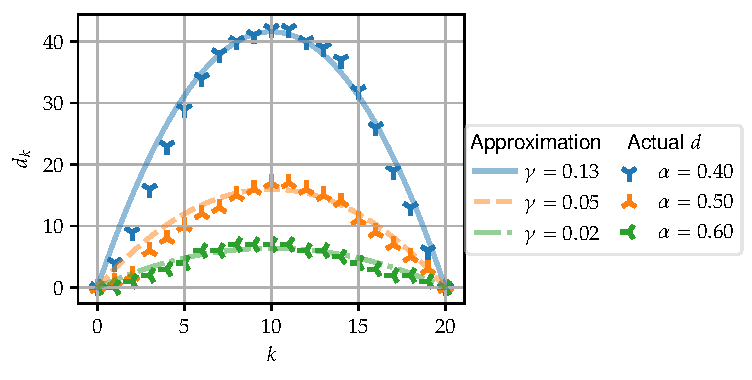
\includegraphics[width=\textwidth]{Plots/approx_degree.pdf}
	\caption{Approximated degree of a matrix from the \emph{Mobilenet V2} model \cite{sandler_mobilenetv2_2019}.
		The actual degree is the number of singular values with $\sigma > \alpha \|A\|_H$ for every causal Hankel matrix. Here $\alpha$ is a hyperparameter that determines the accuracy.
		Additionally approximations of the rank with suitable parameters $\gamma$ are plotted.}
	\label{fig:approx_degree}
\end{figure}
I used an approximation based on the properties of the singular values and their relation to the Frobenius norm.
The singular values are related to the Frobenius norm by $\|H\|_\text{F} = \sqrt{\sum \sigma_i^2}$ \cite[p.~67]{bai_matrix_2021}.
If we suppose that the elements of $H$ have a constant absolute value, then $\|H\|_\text{F} \propto \text{size(H)}$.
This means that the Frobenius norm increases with the size of the matrix, which in turn should also result in increasing singular values.
Finally $d_k$ is the number of singular values larger than a certain threshold value.
The number of states is not directly related to the 2-norm of the singular values as it depends on their distribution and the threshold value.% that depends on wanted accuracy. 
Regardless the approximation $\breve{d}_k \propto \|H_k\|_\text{F}$ fits the behavior of the considered matrices fairly well as illustrated in Figure\,\ref{fig:approx_degree}.
I approximate the degree using the relation
\begin{align}\label{eq:approx_d}
	\breve{d}_k 
	&= \gamma \,\text{size}(H_k) \frac{1}{\min(P,M)}\\
	&= \gamma (K-k+1)(k-1)\frac{PM}{K^2\min(P,M)}.
\end{align}
The variable $\gamma$ is a proportionality factor that represents the required accuracy. 
If a high accuracy is wanted, this results in a higher number of states. 
This can be modeled with a larger $\gamma$.
If we do not need a high accuracy we can use less states.
This is modeled with a smaller $\gamma$.
The factor $1/\min(P,M)$ is used to normalize the state dimensions in such a way that for $\gamma = 1$ the approximation is compatible to the maximum rank of $H_k$. 
As I suppose that the statedimensions for the anticausal case are equivalent to the statedimensions for the causal case, I can calculate the cost using
\begin{equation}
C = \sum_{k=1}^{K} \left(2 d_{k} d_{k+1} + \frac{2 M d_{k+1}}{K} + \frac{2 P d_{k}}{K} + \frac{M P}{K^{2}}\right)
.
\end{equation}
As the matrix can be transposed, $\min(P,M)=M$ can be assumed without loss of generality.
By inserting the approximation from Equation\,\ref{eq:approx_d} and transforming the sums using Faulhaber's formula \cite{knuth_johann_1993} the cost is transformed to
\begin{equation}\label{eq:cost_of_K}
C = \frac{K P^{2} \gamma^{2}}{15} + \frac{M P \gamma}{3} + \frac{P^{2} \gamma}{3} + \frac{M P - \frac{P^{2} \gamma^{2}}{3}}{K} + \frac{- \frac{M P \gamma}{3} - \frac{P^{2} \gamma}{3}}{K^{2}} + \frac{4 P^{2} \gamma^{2}}{15 K^{3}}
.
\end{equation}
This makes it possible, to calculate the cost for different values for the parameter $\gamma$.
In Figure\,\ref{fig:cost_parameters} 
this is done for an example with $M=N = 2^{10}$.
\begin{figure}[htb]
	\centering
	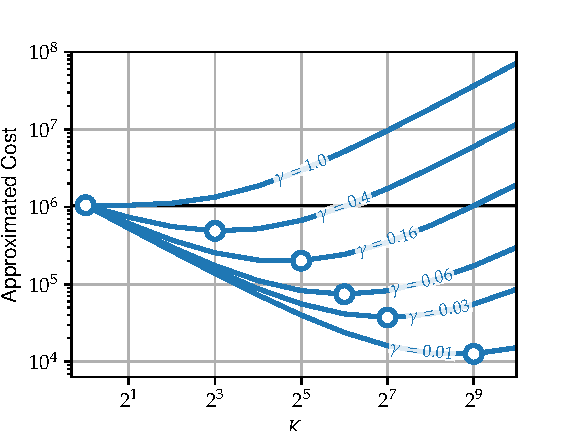
\includegraphics[width=0.75\textwidth]{Plots/cost_parameters.pdf}
	\caption{Approximated cost for different numbers of stages. The system has $M=P=2^{10}$ input and output dimensions. 
	The cost is approximated for different values for the parameter $\gamma$.
	The optimal number of stages for every $\gamma$ is marked with a circle.}
	\label{fig:cost_parameters}
\end{figure}

We can see that for one stage the cost is equivalent to the cost of a simple matrix product, as the whole matrix is stored as one $D$-matrix.
For $\gamma = 1$ the cost only increases for higher number of stages. 
For $\gamma \ll 1$ the cost first decreases before increasing later.
%\todo{Is it usefull to give some details on the parameters of Equation\,\ref{eq:cost_of_K}} 
The figure shows that the optimal number of stages $\hat{K}$ increases as $\gamma$ decreases.
For very small $\gamma$ I get $\hat{K} = 1/2 M$.
For more reasonable values like $\gamma=0.16$ the optimal number of stages is $\hat{K}=2^{-5}M$. 
This gives an educated guess on the optimal number of stages $K$ for a weight matrix.

The approximation has the downsides, that the parameter $\gamma$ has to be estimated
and the input and output dimensions are modeled as constant, which is not true for the tested systems.
%This means that the number of stages can be higher if the stete diemsniuon 
%This is not surprising, as for a high number of stages and a high state dimension, the 
It is also possible to approximate the state dimension based on the maximum possible rank of the Hankel matrix.
The Rank has to be lower than $\min(\text{width}(H_k),\text{height}(H_k))$.
This approximation might have some benefits for very tall or wide matrices, as this approximation is able to represent ranks that are not symmetric in $k$. 


\section{Segmentation Adaptation}\label{sec:Segmentation}

In this section the segmentation of the matrix is changed. 
This means adapting the input and output dimensions. 
First I will describe how to move the boundaries.
In Subsection\,\ref{subsec:move_sig} the algorithm is extended such that makes it possible to calculate the Hankel singular values.
In Subsection\,\ref{subsec:optim_segmentation} a strategy to improve the segmentation is presented.

\subsection{Moving Boundaries}\label{subsec:move}
In this subsection algorithms to move the boundaries of a causal system are introduced.
This is done by changing the segmentation of the input and output.
When we change the segmentation of the input and output, this also changes the segmentation of the transfer matrix $T$.
A change of the division between the inputs $u_k$ and $u_{k+1}$ moves the $k$-th vertical boundary left or right according to
%When we want to movie the $k$-th vertical boundary left or right we change the. 
\makeatletter
\DeclareRobustCommand{\rvdots}{%
  \vbox{
    \baselineskip4\p@\lineskiplimit\z@
    \kern-\p@
    \hbox{.}\hbox{.}\hbox{.}
  }}
\makeatother

\tikzstyle{border} = [line width=1.pt]%[very thick]

\tikzset{
arrow_rl/.pic={
\path[line width=1.5pt,<->] (-3mm,0) edge  (3mm,0);
}
}
\tikzset{
arrow_ud/.pic={
\path[line width=1.5pt,<->] (0,-3mm) edge  (0,3mm);
}
}

\begin{equation}
	\begin{bmatrix}\begin{tikzpicture}
     \matrix [%
       matrix of math nodes,
       column sep=1em,
       row sep=0em,
     ] (y) {%
				\rvdots\\
       y_{k} \\
       y_{k+1} \\
       \rvdots \\
     };


   \end{tikzpicture} \end{bmatrix}
=
\begin{bmatrix}\begin{tikzpicture}
     \matrix [%
       matrix of math nodes,
       column sep=0em,
       row sep=0em
     ] (T) {%
       \ddots&[-0.3em]&&\\
       \cdots&D_k&&\\
       \cdots&B_kC_{k+1}&D_{k+1}&\\[0.75cm,between origins]
       \iddots&\rvdots&\rvdots&\ddots\\
     };



		\node[name=s_line,shape=coordinate] at ($($(T-4-2.south)!0.5!(T-4-3.south)$)+(0.25em,0)$) {};
		\node[name=e_line,shape=coordinate] at ($(s_line)!(T-1-1.north)!($(s_line)+(0,1)$)$) {};
		\draw[border,blue] (s_line) -- (e_line);
		\pic at ($(e_line)-(0,1.5mm)$){arrow_rl};
   \end{tikzpicture} \end{bmatrix}
	\begin{bmatrix}\begin{tikzpicture}
     \matrix [%
       matrix of math nodes,
       column sep=1em,
       row sep=0em,
     ] (u) {%
				\rvdots\\
       u_{k} \\
       u_{k+1} \\
       \rvdots \\
     };

		\node[name=s_line,shape=coordinate] at ($(u-2-1.west)!0.5!(u-3-1.west)$) {};
		\draw[border,blue] (s_line) -- ($(s_line)!(u-3-1.east)!($(s_line)+(1,0)$)$);
    \pic at ($(s_line)+(9mm,0)$){arrow_ud};
   \end{tikzpicture} \end{bmatrix}
\end{equation}



A change of the division between the outputs $y_k$ and $y_{k+1}$ analogously moves the $k$-th horizontal boundary up or down according to
\makeatletter
\DeclareRobustCommand{\rvdots}{%
  \vbox{
    \baselineskip4\p@\lineskiplimit\z@
    \kern-\p@
    \hbox{.}\hbox{.}\hbox{.}
  }}
\makeatother

\tikzstyle{border} = [line width=1.pt]%[very thick]

\tikzset{
arrow_rl/.pic={
\path[line width=1.5pt,<->] (-3mm,0) edge  (3mm,0);
}
}
\tikzset{
arrow_ud/.pic={
\path[line width=1.5pt,<->] (0,-3mm) edge  (0,3mm);
}
}

\begin{equation}
	\begin{bmatrix}\begin{tikzpicture}
     \matrix [%
       matrix of math nodes,
       column sep=1em,
       row sep=0em,
     ] (y) {%
				\rvdots\\
       y_{k} \\
       y_{k+1} \\
       \rvdots \\
     };

		\node[name=s_line,shape=coordinate] at ($(y-2-1.west)!0.5!(y-3-1.west)$) {};
		\draw[border,blue] (s_line) -- ($(s_line)!(y-3-1.east)!($(s_line)+(1,0)$)$);
    \pic at ($(s_line)+(9mm,0)$){arrow_ud};
   \end{tikzpicture} \end{bmatrix}
=
\begin{bmatrix}\begin{tikzpicture}
     \matrix [%
       matrix of math nodes,
       column sep=0em,
       row sep=0em
     ] (T) {%
       \ddots&[-0.3em]&&\\
       \cdots&D_k&&\\
       \cdots&B_kC_{k+1}&D_{k+1}&\\[0.75cm,between origins]
       \iddots&\rvdots&\rvdots&\ddots\\
     };

		\node[name=s_line,shape=coordinate] at ($($(T-2-1.west)!0.5!(T-3-1.west)$)+(0,0.1em)$) {};
    \node[name=e_line,shape=coordinate] at ($(s_line)!(T-4-4.east)!($(s_line)+(1,0)$)$) {};
		\draw[border,blue] (s_line) -- (e_line);
    \pic at ($(e_line)-(1.5mm,0)$){arrow_ud};


   \end{tikzpicture} \end{bmatrix}
	\begin{bmatrix}\begin{tikzpicture}
     \matrix [%
       matrix of math nodes,
       column sep=1em,
       row sep=0em,
     ] (u) {%
				\rvdots\\
       u_{k} \\
       u_{k+1} \\
       \rvdots \\
     };

   \end{tikzpicture} \end{bmatrix}
\end{equation}



%To move the  we change the .
%This means moving the input $u_\m$ or output $y_\m$ from one stage to another.
%The connections that are changed when we do this are drawn in color in the Figures\,\ref{fig:move_left}-\ref{fig:move_up}.
%If we move the boundaries we make sure, that the connections from the previous state $x_k$ to the combined output $y$ and the connections form the combined input $u$ to the next state $x_{k+1}$ stay unchanged.
%This also means that the observability and reachability matrices for the previous and later states are invariant under the movement of the boundary.
%This results in the fact that minimality of these states stays unchanged.
The movement of the boundaries changes the parts of the matrix that can be represented with a causal system.
When we move boundaries to the left or down, some connections are no longer possible in a causal system. These will be dropped.
Conversely when we move boundaries to the right or up, new connections will be established.
%These connections will be drawn with dotted lines in the Figures\,\ref{fig:move_left}-\ref{fig:move_up}.
For a mixed system these connections can be moved to the anticausal system and vice versa.
The algorithms are constructed such that they also preserve the minimality of the system.%intermediate state $x_{k+1}$.
%\todo[inline]{deeper explination needed?}

\paragraph{Move Left}
\begin{figure}[!htb]
	\centering
	\begin{tikzpicture}[font=\small,fontmatrices=\small,boxsize=12mm]

\tikzstyle{colmarking} = [magenta!50!violet!100,line width=1.5pt]
\def\colortext{magenta!50!violet!100}


\def\distorig{\rel_i_stage*\pgfkeysvalueof{/tikz/boxsize}}
\def\distvert{3mm}
%\def

	\matrix (m1) [row sep=5.mm, column sep=9mm] at (-3.2,0)
	{
		&		\node[coordinate]  (xin) {}; & \\[1.2cm,between origins]
		%--------------------------------------------------------------------
		\node[]                  (u_1) {$u_{k}$};          &
		\node[style_stage, stage, name=sys_1,A=$A_{1}$,B=$$,C=$$,D=$$] {};&
		\node[]                  (y_1) {$y_k$};          \\
		%--------------------------------------------------------------------
		\node[]                  (u_2) {$u_{k+1}$};          &
		\node[style_stage, stage, name=sys_2,A=$\textcolor{\colortext}{A_{k+1}}$,B=$$,C=$\!\textcolor{\colortext}{C_{k+1}}$,D=$$] {};&
		\node[]                  (y_2) {$y_{k+1}$};          \\[1.4cm,between origins]

		 &		\node[coordinate]  (xout) {}; & \\
	};


	\foreach \i in {1,2}
		{
		  \draw[signalflow] (u_\i) -- (sys_\i.u);
	  	\draw[signalflow] (sys_\i.y) -- (y_\i);
		}
	\draw[signalflow] (xin)                      -- node[anchor = west]          {$x_{k}$} (sys_1.xin);
	\draw[signalflow] (sys_1.xout)               -- node[anchor=west]            {$x_{k+1}$} (sys_2.xin);
	\draw[signalflow] (sys_2.xout)               -- node[near end,anchor = west] {$x_{k+2}$} (xout);

\draw[signalflow, colmarking] (u_1) to [out=0,in=180] node[near end,anchor = north] {$u_\m$} ($(sys_1.u)+(0,-\distvert)$)-- ($(sys_1.center)+(-\distorig,-\distvert)$); 
 %\draw[signalflow, colmarking] ($(u_1.east)+(0,-\distvert)$) -- ($(sys_1.u)+(0,-\distvert)$);
 \draw[signal,colmarking] ($(sys_1.u)+(0,-\distvert)$)-- ($(sys_1.center)+(0.5*\distorig,-\distvert)$);
 \draw[signalflow, colmarking] ($(sys_1.center)+(0.5*\distorig,-\distvert)$)  to [out=0,in=180] node[anchor=north] {$d$} (sys_1.east);


 \draw[signalflow,colmarking] ($(sys_1.center)+(-\distorig,-\distvert)$) -- node[anchor=north east] {$b$} ($(sys_1.center)+(0,-\distorig-\distvert)$)  ; 

 \draw[signal,colmarking] ($(sys_1.center)+(0,-\distorig-\distvert)$) -- (sys_2.xout);
 \draw[signal,colmarking] ($(sys_2.center)+(0,\distorig)$) -- ($(sys_2.center)+(\distorig,0)$) -- (sys_2.y);




	\matrix (m1) [row sep=5.mm, column sep=9mm] at (3.2,0)
	{
		&		\node[coordinate]  (xin) {}; & \\[1.2cm,between origins]
		%--------------------------------------------------------------------
		\node[]                  (u_1) {$\tilde{u}_{k}$};          &
		\node[style_stage, stage, name=sys_1,A=$\tilde{A}_k$,B=$\tilde{B}_{k}$,C=$C_{k}$,D=$\tilde{D}_{k}$] {};&
		\node[]                  (y_1) {$y_{k}$};          \\
		%--------------------------------------------------------------------
		\node[]                  (u_2) {$\tilde{u}_{k+1}$};          &
		\node[style_stage, stage, name=sys_2,A=$$,B=$$,C=$$,D=$$] {};&
		\node[]                  (y_2) {$y_{k+1}$};          \\[1.4cm,between origins]

		 &		\node[coordinate]  (xout) {}; & \\
	};


	\foreach \i in {1,2}
		{
		  \draw[signalflow] (u_\i) -- (sys_\i.u);
	  	\draw[signalflow] (sys_\i.y) -- (y_\i);
		}
	\draw[signalflow] (xin)                      -- node[anchor = west]          {$x_k$} (sys_1.xin);
	\draw[signalflow] (sys_1.xout)               -- node[anchor=west]            {$\tilde{x}_{k+1}$} (sys_2.xin);
	\draw[signalflow] (sys_2.xout)               -- node[near end,anchor = west] {$x_{k+2}$} (xout);

%d-connection
\draw[signalflow, colmarking] (u_2) to [out=0,in=180] node[near end,anchor = south] {$u_\m$} ($(sys_2.u)+(0,+\distvert)$)-- ($(sys_2.center)+(-\distorig,+\distvert)$); 
%\draw[signalflow, colmarking] ($(u_2.east)+(0,\distvert)$) --  ($(sys_2.u)+(0,\distvert)$);
\draw[signal,colmarking] ($(sys_2.u)+(0,\distvert)$)--($(sys_2.center)+(0.5*\distorig,\distvert)$);
 \draw[signalflow, colmarking] ($(sys_2.center)+(0.5*\distorig,\distvert)$) to [out=0,in=180] node[name=Cb] {} (sys_2.y);

%diagonal
 \draw[signalflow,colmarking] ($(sys_2.center)+(-\distorig,\distvert)$) -- node[name=Ab]   {} ($(sys_2.center)+(0,-\distorig+\distvert)$)  ; 
%down
\draw[signal,colmarking] ($(sys_2.center)+(0,-\distorig+\distvert)$) -- (sys_2.xout);

\node (Abtext) at ($(sys_2.center)+(-\distorig,-\distorig)$) {$\;\,\textcolor{\colortext}{A_{k+1}b}$};
\node (Cbtext) at ($(sys_2.center)+(\distorig,\distorig)$) {$\!\!\textcolor{\colortext}{C_{k+1}b}$};

\draw[white,line width=1mm,opacity=0.8] (Abtext) to [out=80,in=200] (Ab);
\draw[colmarking,line width=0.7pt] (Abtext) to [out=80,in=200] (Ab);

\draw[colmarking,line width=0.7pt] (Cbtext) to [out=-80,in=40] ($(Cb.center)+(1mm,0.5mm)$);
\end{tikzpicture}
	\begin{subfigure}[b]{0.45\textwidth}
		\caption{Original system}
		\label{fig:move_left_a}
	\end{subfigure}
	\hspace{0.8cm}
	\begin{subfigure}[b]{0.45\textwidth}
		\caption{Moved system}
		\label{fig:move_left_b}
	\end{subfigure}
	\caption{Illustration of a system where a boundary is moved to the left}
	\label{fig:move_left}
\end{figure}
\begin{algorithm}[!htb]
	\begin{algorithmic}
		\Input{System $\Sigma_{[A,B,C,D]}$, Index $k$, Tolerance $\text{tol}$ }
		\Output{System $\Sigma_{[A,B,C,D]}$ with changed input dimensions}
		\State $b \gets B_{k[:,\en]}$
		\State $D_k \gets D_{k[:,:\en-1]}$
		\State $B_k \gets B_{k[:,:\en-1]}$
		\State $D_{k+1} \gets [C_{k+1}b,D_{k+1}]$
		\State $B_{k+1} \gets [A_{k+1}b,B_{k+1}]$
		\State $U,\sigma,V^\top \gets$ SVD$([A_k,B_k],\text{econ}=\text{True})$ 
		\If{$\sigma_{[\en-1]} < \text{tol}$}
		\State $U \gets U_{[:,:\en-1]}$; $\sigma \gets \sigma_{[:\en-1]}$; $V \gets V_{[:,:\en-1]}$
		%\State $U \gets U[:,:-2]$
		%\State $\sigma \gets \sigma[:-2]$
		%\State $V \gets V[:-2,:]$
		\State$[A_k,B_k] \gets \diag(\sigma) V^\top$
		\State$A_{k+1} \gets A_{k+1}U$
		\State$C_{k+1} \gets C_{k+1}U$
		\EndIf
	\end{algorithmic}
	\caption{Algorithm to move a boundary between $u_k$ and $u_{k+1}$ to the left}\label{alg:move_left}
\end{algorithm}
First we move the $k$-th vertical boundary to the left.
This means that the last element of the input $u_k$ becomes the first element in $u_{k+1}$. 
This moved input is designated as $u_\m$.
The altered connections are drawn in color in Figure\,\ref{fig:move_left}.

The vector $b$ is the last column of $B_k$ and describes the connection from $u_\m$ to $x_{k+1}$. The vector $d$ is the last column of $D_k$ and describes the connection from $u_\m$ to $y_{k}$.
These vectors are removed from the matrices and we get $\breve{B}_k$ and $\tilde{D}$.
We can see that the connection $d$ in the original system cannot by realized with a causal system as this would mean a connection from $\tilde{u}_{k+1}$ to $y_k$ in the transformed system.
This also means that the parts of the transfer matrix $T$ that can be represented using the causal system change.
The dropped connection is illustrated using a dotted line in Figure\,\ref{fig:move_left}.
Now we have to add the the input $u_\m$ to the next stage.
The connection from the input $u_\m$ to the output $y_{k+1}$ can be incorporated by adding the vector $C_{k+1}b$ to $D_{k+1}$ as a new column.
Analogously the connection from $u_\m$ to the state $x_{k+2}$ can be incorporated by attaching the vector $A_{k+1}b$ to $B_{k+1}$.

After these changes, the mapping from the combined inputs $[u_k^\top \: u_{k+1}^\top]^\top$
to the state $x_{k+2}$ remains unchanged. Therefore the following states are still reachable and minimal. 
As the last column of $\R_{k+1}$ is removed, the state $x_{k+1}$ might become non reachable.
This is the case if the matrix $[A_b \: \breve{B}_k]$ does no longer has full rank.
We can check this using the SVD. 
If the last singular value is equal to zero, one statedimension has to be removed. 
This can be done using a state transformation based on the reduced SVD. 
The matrices $[\tilde{A}_b \: \tilde{B}_k]$ are set to $\diag(\sigma) V^\top$ and 
the following stages are transformed according to $\tilde{A}_{k+1} = A_{k+1}U$ and $\tilde{C}_{k+1} = C_{k+1} U$.
This restores the minimality of the system.

The pseudocode to move the boundary to the left is given in Algorithm\,\ref{alg:move_left}.
 


\paragraph{Move Down}
\begin{figure}[!htb]
	\centering
	\begin{tikzpicture}[font=\small,fontmatrices=\small,boxsize=12mm]
%violet!80!red!90
\tikzstyle{colmarking} = [magenta!50!violet!100,line width=1.5pt]
\def\colortext{magenta!50!violet!100}


\def\distorig{\rel_i_stage*\pgfkeysvalueof{/tikz/boxsize}}
\def\distvert{3mm}
%\def

	\matrix (m1) [row sep=5.mm, column sep=9mm] at (-3.2,0)
	{
		&		\node[coordinate]  (xin) {}; & \\[1.2cm,between origins]
		%--------------------------------------------------------------------
		\node[]                  (u_1) {$u_{k}$};          &
		\node[style_stage, stage, name=sys_1,A=$\textcolor{\colortext}{A_{k}}$,B=$\textcolor{\colortext}{B_k}$,C=$$,D=$$] {};&
		\node[]                  (y_1) {$y_k$};          \\
		%--------------------------------------------------------------------
		\node[]                  (u_2) {$u_{k+1}$};          &
		\node[style_stage, stage, name=sys_2,A=$$,B=$$,C=$$,D=$$] {};&
		\node[]                  (y_2) {$y_{k+1}$};          \\[1.4cm,between origins]

		 &		\node[coordinate]  (xout) {}; & \\
	};


	\foreach \i in {1,2}
		{
		  \draw[signalflow] (u_\i) -- (sys_\i.u);
	  	\draw[signalflow] (sys_\i.y) -- (y_\i);
		}
	\draw[signalflow] (xin)                      -- node[anchor = west]          {$x_{k}$} (sys_1.xin);
	\draw[signalflow] (sys_1.xout)               -- node[anchor=west]            {$x_{k+1}$} (sys_2.xin);
	\draw[signalflow] (sys_2.xout)               -- node[near end,anchor = west] {$x_{k+2}$} (xout);

%dconnection
\draw[signalflow, colmarking]  ($(sys_2.center)+(\distorig,\distvert)$) -- ($(sys_2.y)+(0,\distvert)$) to [out=0,in=180] node[near end,anchor = south] {$y_\m$} (y_2) ; 
 %\draw[signalflow, colmarking] ($(u_1.east)+(0,-\distvert)$) -- ($(sys_1.u)+(0,-\distvert)$);
 \draw[signal,colmarking,dotted] ($(sys_2.y)+(0,\distvert)$)-- ($(sys_2.center)+(-0.5*\distorig,\distvert)$);
 \draw[signalflow, colmarking,dotted] (sys_2.west)   to [out=0,in=180] node[anchor=south] {$d$} ($(sys_2.center)+(-0.5*\distorig,\distvert)$);

%diagonal c
 \draw[signalflow,colmarking,line cap=round] ($(sys_2.center)+(0,\distorig+\distvert)$) -- node[near end,anchor=south west] {$\!\!c^\top$}   ($(sys_2.center)+(\distorig,\distvert)$); 
%connect systems
\draw[signal,colmarking] ($(sys_2.center)+(0,\distorig+\distvert)$) -- (sys_1.xin);
%B_k
\draw[signal,colmarking] (sys_1.u) -- ($(sys_1.center)+(-\distorig,0)$) -- ($(sys_1.center)+(0,-\distorig)$);




	\matrix (m1) [row sep=5.mm, column sep=9mm] at (3.2,0)
	{
		&		\node[coordinate]  (xin) {}; & \\[1.2cm,between origins]
		%--------------------------------------------------------------------
		\node[]                  (u_1) {${u}_{k}$};          &
		\node[style_stage, stage, name=sys_1,A=$\tilde{A}_k$,B=$\tilde{B}_{k}$,C=$$,D=$$] {};&
		\node[]                  (y_1) {$\tilde{y}_{k}$};          \\
		%--------------------------------------------------------------------
		\node[]                  (u_2) {${u}_{k+1}$};          &
		\node[style_stage, stage, name=sys_2,A=$$,B=$$,C=$$,D=$$] {};&
		\node[]                  (y_2) {$\tilde{y}_{k+1}$};          \\[1.4cm,between origins]

		 &		\node[coordinate]  (xout) {}; & \\
	};


	\foreach \i in {1,2}
		{
		  \draw[signalflow] (u_\i) -- (sys_\i.u);
	  	\draw[signalflow] (sys_\i.y) -- (y_\i);
		}
	\draw[signalflow] (xin)                      -- node[anchor = west]          {$x_k$} (sys_1.xin);
	\draw[signalflow] (sys_1.xout)               -- node[anchor=west]            {$\tilde{x}_{k+1}$} (sys_2.xin);
	\draw[signalflow] (sys_2.xout)               -- node[near end,anchor = west] {$x_{k+2}$} (xout);

%shade behind diag
\draw[white,line width=2.5mm,opacity=0.8] ($(sys_1.center)+(-1mm,1mm+\distorig-\distvert)$) -- ($(sys_1.center)+(\distorig,-\distvert)$); 

%dconnection
\draw[signalflow, colmarking]  ($(sys_1.center)+(\distorig,-\distvert)$) -- ($(sys_1.y)+(0,-\distvert)$) to [out=0,in=180] node[near end,anchor = south] {$y_\m$} (y_1) ; 
 %\draw[signalflow, colmarking] ($(u_1.east)+(0,-\distvert)$) -- ($(sys_1.u)+(0,-\distvert)$);
 \draw[signalflow,colmarking] ($(sys_1.center)+(0,-\distvert)$) -- node[anchor=north] {$c^\top \!B_k$} ($(sys_1.y)+(0,-\distvert)$);
 \draw[signal, colmarking] (sys_1.west) --  ($(sys_1.center)+(-\distorig,0)$)  to [out=0,in=180]  ($(sys_1.center)+(0,-\distvert)$);

%diagonal
\draw[signalflow,colmarking,line cap=round] ($(sys_1.center)+(0,\distorig-\distvert)$) -- node[name=Cb]   {} ($(sys_1.center)+(\distorig,-\distvert)$)  ; 
 \draw[signal,colmarking] (sys_1.xin) -- ($(sys_1.center)+(0,\distorig-\distvert)$);

%\node (Abtext) at ($(sys_2.center)+(-\distorig,-\distorig)$) {$\;\,\textcolor{\colortext}{A_{k+1}b}$};
\node (Cbtext) at ($(sys_1.center)+(\distorig,\distorig)$) {$\!\!\textcolor{\colortext}{C_{k+1}b}$};

\draw[white,line width=1mm,opacity=0.8] (Cbtext) to [out=280,in=80] (Cb);
\draw[colmarking,line width=0.7pt] (Cbtext) to [out=280,in=80] (Cb);

%\draw[colmarking] (Cbtext) to [out=-80,in=40] ($(Cb.center)+(1mm,0.5mm)$);
\end{tikzpicture}
	\begin{subfigure}[b]{0.45\textwidth}
		\caption{Original system}
		\label{fig:move_down_a}
	\end{subfigure}
	\hspace{0.8cm}
	\begin{subfigure}[b]{0.45\textwidth}
		\caption{Moved system}
		\label{fig:move_down_b}
	\end{subfigure}
	\caption{Illustration of a system where a boundary is moved down}
	\label{fig:move_down}
\end{figure}
\begin{algorithm}[!htb]
	\begin{algorithmic}
		\Input{System $\Sigma_{[A,B,C,D]}$, Index $k$, Tolerance $\text{tol}$ }
		\Output{System $\Sigma_{[A,B,C,D]}$ with changed output dimensions}
		\State $c^\top \gets C_{k+1[1,:]}$
		\State $D_{k+1} \gets D_{k+1[2:,]}$
		\State $C_{k+1} \gets C_{k+1[2:,:]}$
		\State $D_k \gets \begin{bmatrix} D_k\\c^\top B_k	\end{bmatrix}$
		\State $C_k \gets \begin{bmatrix} C_k\\c^\top A_k	\end{bmatrix}$
		\State $U,\sigma,V^\top \gets$ SVD$\left(\begin{bmatrix} A_{k+1}\\C_{k+1}	\end{bmatrix},\text{econ}=\text{True}\right)$ 
		\If{$\sigma_{[\en]} < \text{tol}$}
		\State $U \gets U_{[:,:\en-1]}$; $\sigma \gets \sigma_{[:\en-1]}$; $V \gets V_{[:,:\en-1]}$
		%\State $U \gets U[:,:-2]$
		%\State $\sigma \gets \sigma[:-2]$
		%\State $V \gets V[:-2,:]$
		\State$\begin{bmatrix} A_{k+1}\\C_{k+1}	\end{bmatrix} \gets U\diag(\sigma)$
		\State$A_{k} \gets V^\top A_{k}$
		\State$C_{k} \gets V^\top C_{k}$
		\EndIf
	\end{algorithmic}
	\caption{Algorithm to move a boundary between $y_k$ and $y_{k+1}$ down}\label{alg:move_down}
\end{algorithm}
A similar strategy can be used to move the $k$-th horizontal a boundary down.
That means moving the first output $y_\m$ from $y_{k+1}$ to $y_k$.
The altered connections are drawn in color in Figure\,\ref{fig:move_down}.

The vector $c^\top$ is the first row of $C_{k+1}$ and describes the connection from $x_k$ to $y_\m$.
This vector is removed from $C_{k+1}$.
We also remove the first row from $D_{k+1}$.
The dotted connection from $u_{k+1}$ to the output $y_\m$ is no longer possible and therefore we have to drop it.
Now we attach the output $y_\m$ to the output vector $y_k$.
For this the vector $c^\top B_k$ is added as last row to $D_k$ and the vector $c^\top A_k$ is added as last row to $C_k$.

The mapping from the state $x_k$ to the combined outputs $[y_k^\top \: y_{k+1}^\top]^\top$ remains unchanged. This means that the previous states are still observable and therefore minimal. 
As the algorithm removes a row from $\Ob_{k+1}$ it might happen that the state $x_{k+1}$ is no longer observable.
This is the case if the kernel of $\Ob_{k+1}$ is not the zero subspace.
We can check this with the SVD of $[A_{k+1}^\top,\breve{C}_{k+1}^\top]^\top$.
If the last singular value is equal to zero one state dimension has to be removed.
This is done by using a state transformation based on the reduced SVD. 
Again the inverse does not need to be calculated as it is implicitly calculated by the SVD.
An algorithm to move the state is given in Algorithm\,\ref{alg:move_down}.

\FloatBarrier
\paragraph{Move Right}
\begin{figure}[!htb]
	\centering
	\begin{tikzpicture}[font=\small,fontmatrices=\small,boxsize=11mm]
%violet!80!red!90
\tikzstyle{colmarking} = [magenta!50!violet!100,line width=1.5pt]
\def\colortext{magenta!50!violet!100}


\def\distorig{\rel_i_stage*\pgfkeysvalueof{/tikz/boxsize}}
\def\distvert{2.7mm}
%\def

	\matrix (m1) [row sep=5.mm, column sep=9mm] at (-3.2,0)
	{
		&		\node[coordinate]  (xin) {}; & \\[1.2cm,between origins]
		%--------------------------------------------------------------------
		\node[]                  (u_1) {$u_{k}$};          &
		\node[style_stage, stage, name=sys_1,A=$$,B=$$,C=$$,D=$$] {};&
		\node[]                  (y_1) {$y_k$};          \\
		%--------------------------------------------------------------------
		\node[]                  (u_2) {$u_{k+1}$};          &
		\node[style_stage, stage, name=sys_2,A=$$,B=$$,C=$$,D=$$] {};&
		\node[]                  (y_2) {$y_{k+1}$};          \\[1.4cm,between origins]

		 &		\node[coordinate]  (xout) {}; & \\
	};


	\foreach \i in {1,2}
		{
		  \draw[signalflow] (u_\i) -- (sys_\i.u);
	  	\draw[signalflow] (sys_\i.y) -- (y_\i);
		}
	\draw[signalflow] (xin)                      -- node[anchor = west]          {$x_{k}$} (sys_1.xin);
	\draw[signalflow] (sys_1.xout)               -- node[anchor=west]            {$x_{k+1}$} (sys_2.xin);
	\draw[signalflow] (sys_2.xout)               -- node[near end,anchor = west] {$x_{k+2}$} (xout);


%d-connection
\draw[signalflow, colmarking] (u_2) to [out=0,in=180] node[near end,anchor = south] {$u_\m$} ($(sys_2.u)+(0,+\distvert)$)-- ($(sys_2.center)+(-\distorig,+\distvert)$);
%\draw[signalflow, colmarking] ($(u_2.east)+(0,\distvert)$) --  ($(sys_2.u)+(0,\distvert)$);
\draw[signalflow,colmarking] ($(sys_2.u)+(0,\distvert)$)--node[anchor=south] {$d$} ($(sys_2.center)+(0.5*\distorig,\distvert)$);
 \draw[signal, colmarking] ($(sys_2.center)+(0.5*\distorig,\distvert)$) to [out=0,in=180] (sys_2.y);

%diagonal
 \draw[signalflow,colmarking,line cap=round] ($(sys_2.center)+(-\distorig,\distvert)$) -- node[name=b,pos = 0.5]   {} ($(sys_2.center)+(0,-\distorig+\distvert)$)  ;
%down
\draw[signal,colmarking] ($(sys_2.center)+(0,-\distorig+\distvert)$) -- (sys_2.xout);

\node (btext) at ($(sys_2.center)+(-\distorig,-\distorig)$) {$\;\textcolor{\colortext}{b}$};

\draw[white,line width=1mm,opacity=0.8] (btext) to [out=80,in=200] (b);
\draw[colmarking,line width=0.7pt] (btext) to [out=80,in=200] (b);



	\matrix (m1) [row sep=5.mm, column sep=9mm] at (3.2,0)
	{
		&		\node[coordinate]  (xin) {}; & \\[1.2cm,between origins]
		%--------------------------------------------------------------------
		\node[]                  (u_1) {$\tilde{u}_{k}$};          &
		\node[style_stage, stage, name=sys_1,A=$\tilde{A}_k$,B=$$,C=$$,D=$$] {};&
		\node[]                  (y_1) {${y}_{k}$};          \\
		%--------------------------------------------------------------------
		\node[]                  (u_2) {$\tilde{u}_{k+1}$};          &
		\node[style_stage, stage, name=sys_2,A=$$,B=$$,C=$$,D=$$] {};&
		\node[]                  (y_2) {${y}_{k+1}$};          \\[1.4cm,between origins]

		 &		\node[coordinate]  (xout) {}; & \\
	};


	\foreach \i in {1,2}
		{
		  \draw[signalflow] (u_\i) -- (sys_\i.u);
	  	\draw[signalflow] (sys_\i.y) -- (y_\i);
		}
	\draw[signalflow] (xin)                      -- node[anchor = west]          {$x_k$} (sys_1.xin);
	\draw[signalflow] (sys_1.xout)               -- node[anchor=west]            {$\tilde{x}_{k+1}$} (sys_2.xin);
	\draw[signalflow] (sys_2.xout)               -- node[near end,anchor = west] {$x_{k+2}$} (xout);


\draw[white,line width=2.5mm,opacity=0.8] ($(sys_2.center)+(-\distvert,\distorig)$) -- ($(sys_2.center)+(\distorig-\distvert,0)$)  ;

\draw[signalflow, colmarking] (u_1) to [out=0,in=180] node[near end,anchor = north] {$u_\m$} ($(sys_1.u)+(0,-\distvert)$)-- ($(sys_1.center)+(-\distorig,-\distvert)$);
 %\draw[signalflow, colmarking] ($(u_1.east)+(0,-\distvert)$) -- ($(sys_1.u)+(0,-\distvert)$);
 \draw[signal,colmarking,dotted] ($(sys_1.u)+(0,-\distvert)$)-- ($(sys_1.center)+(0.5*\distorig,-\distvert)$);
 \draw[signalflow, colmarking,dotted] ($(sys_1.center)+(0.5*\distorig,-\distvert)$)  to [out=0,in=180] node[anchor=north] {$d_{\text{new}}$} (sys_1.east);

%diag eye
\draw[signal,colmarking,line cap=round] ($(sys_1.center)+(-\distorig,-\distvert)$) --  ($(sys_1.center)+(-\distvert,-\distorig)$)  ;
\draw[signalflow,colmarking] ($(sys_1.center)+(-\distvert,-\distorig)$) -- ($(sys_2.center)+(-\distvert,\distorig)$);
%dia_d
\draw[signalflow,colmarking,line cap=round] ($(sys_2.center)+(-\distvert,\distorig)$) -- node[name=d]   {} ($(sys_2.center)+(\distorig-\distvert,0)$)  ;
\draw[signal,colmarking] ($(sys_2.center)+(\distorig-\distvert,0)$) -- (sys_2.y);
%back to x
\draw[signalflow,colmarking] ($(sys_2.center)+(-\distvert,\distorig)$)-- ($(sys_2.center)+(-\distvert,\distvert)$) to [out=270,in=90] node[name=b] {} ($(sys_2.center)+(-0,-\distorig)$) -- (sys_2.xout);
\node (btext) at ($(sys_2.center)+(-\distorig,-\distorig)$) {$\;\;\textcolor{\colortext}{b}$};
\node (dtext) at ($(sys_2.center)+(\distorig,\distorig)$) {$\!\textcolor{\colortext}{d}$};

\draw[white,line width=1mm,opacity=0.8] (btext) to [out=60,in=180] (b);
\draw[colmarking,line width=0.7pt] (btext) to [out=60,in=180] (b);

\draw[white,line width=1mm,opacity=0.8] (dtext) to [out=180,in=80] (d);
\draw[colmarking,line width=0.7pt] (dtext) to [out=180,in=80] (d);


\end{tikzpicture}

	\begin{subfigure}[b]{0.45\textwidth}
		\caption{Original system}
		\label{fig:move_right_a}
	\end{subfigure}
	\hspace{0.8cm}
	\begin{subfigure}[b]{0.45\textwidth}
		\caption{Moved system}
		\label{fig:move_right_b}
	\end{subfigure}
	\caption{Illustration of a system where a boundary is moved to the right}
	\label{fig:move_right}
\end{figure}
\begin{algorithm}[!htb]
	\begin{algorithmic}
		%		def move_right(sys,v,d_new=None):
		%		#function to move a boundary left 
		%		#v is the index to the left of the boundary
		\Input{System $\Sigma_{[A,B,C,D]}$, Index $k$, Tolerance $\text{tol}$} 
		\Output{System $\Sigma_{[A,B,C,D]}$ with changed input dimensions}
		\State $b \gets B_{k+1[:,1]}$
		\State $d \gets D_{k+1[:,1]}$
		\State $B_{k+1} \gets B_{k+1[:,2:]}$
		\State $D_{k+1} \gets D_{k+1[:,2:]}$
		%		#check if [d;b] in range(C_v+1;Av+1)
		\State $U,\sigma,V^\top \gets$ SVD$\left(\begin{bmatrix}
		C_{k+1}\\A_{k+1}
		\end{bmatrix}\right)$ 
		
		\State $r \gets $ count$(\sigma>\text{tol}_i)$
		\State $a \gets U^\top \begin{bmatrix}
		d\\b
		\end{bmatrix}$
		%\If{any $|a[r+1:]|>\text{tol}$}
		\If{$\|a_{[r+1:]}\|>\text{tol}$}
		\Comment not in range
		\State $B_k \gets \begin{bmatrix}
		B_k & 0\\
		0 & 1
		\end{bmatrix}$
		\State $A_k \gets \begin{bmatrix}
		A_k \\ 0
		\end{bmatrix}$
		\State $A_{k+1} \gets [A_{k+1},b]$
		\State $C_{k+1} \gets [C_{k+1},d]$		
		\Else
		%			#in range -> no need for an additional dim
		\State $m \gets V_{[:,:r]} \diag(\sigma_{[:r]})^{-1} a_{[:r]}$
		\State $B_k \gets \begin{bmatrix} B_k & m\end{bmatrix}$
		%		
		\EndIf
		%		#set the appropirate D_v
		\State $D_k \gets \begin{bmatrix}
		D_k&d_{\text{new}}
		\end{bmatrix}$
	\end{algorithmic}
	\caption{Algorithm to move a boundary between $u_k$ and $u_{k+1}$ to the right}\label{alg:move_right}
\end{algorithm}
It is also possible to reverse these changes.
When we move the $k$-th vertical boundary to the right, the input $u_\m$ is moved from $u_{k+1}$ to $\tilde{u}_k$.
The connection from $u_\m$ is moved from the current stage to the previous stage.
We can do this by directly routing the input to an additional state dimension.
To attach the input $u_\m$ to the end of the state vector $x_{k+1}$, we set 
\begin{equation}
	\breve{B}_k = \begin{bmatrix}
	B_k & 0\\
	0 & 1
	\end{bmatrix}
\end{equation}
This makes the input $u_\m$ available in the next stage.
Now the connections can be reconnected.
For this we remove first row $d$ of $D_{k+1}$ and attach it to $C_{k+1}$ as the new last row. 
Analogously the first row $b$ of $B_{k+1}$ is removed and attached to the end of $A_{k+1}$.
This is illustrated in Figure\,\ref{fig:move_right}.

After these changes, the mapping from the combined inputs $[u_k^\top \: u_{k+1}^\top]^\top$
to the state $x_{k+2}$ remains unchanged. Therefore the following states are still reachable and minimal.
This trivial approach results in a new observability matrix $\tilde{\Ob}_{k+1}$ and a reachability matrix $\tilde{\R}_{k+1}$ for the state $x_{k+1}$.
The state $x_k$ is still reachable, as the additional statedimension is directly connected to the input $u_\m$.
The observability matrix has one additional column
\begin{equation}\label{eq:strucure_mover}
	\tilde{\Ob}_{k+1}
	=
	\begin{bmatrix}
	\eye & 0\\ 0 &\Ob_{k+2}
	\end{bmatrix}
	\begin{bmatrix}
	C_{k+1} & d\\
	A_{k+1} & b
	\end{bmatrix}
	.
\end{equation}
If the last column is not linearly independent, the system is no longer observable as $\Ob_{k+1}$ does not have full column rank.
This is the case if
\begin{equation}
	\begin{bmatrix}
	d\\b
	\end{bmatrix}
	\in
	\range\left(
	\begin{bmatrix}
	C_{k+1}\\A_{k+1}
	\end{bmatrix}\right).
\end{equation}
If the vector is in the range then a state $m$ with the property
\begin{equation}
	\begin{bmatrix}
	d\\b
	\end{bmatrix}
	=
	\begin{bmatrix}
	C_{k+1}\\A_{k+1}
	\end{bmatrix}
	m
\end{equation}
exists.
This also means that no new state dimension is required.
In this case the vector $m$ is appended to the matrix $B_{k}$.
The algorithm uses the SVD of $[C_{k+1}^\top,A_{k+1}^\top]^\top$ to check the relations.
This uses the intermediate vector 
\begin{equation}
	a = U^\top 	
	\begin{bmatrix}
	d\\b
	\end{bmatrix}
\end{equation} 
If the vector $[d^\top,b^\top]^\top$ is in the range, the norm of 
\begin{equation}
	\|a_{[r+1:]} \| = 0
	.
\end{equation}
Here $r$ is the number of nonzero singular values.
The vector $m$ is computed with 
\begin{equation}
	m = V_{[:,:r]} \diag(\sigma_{[:r]})^{-1} a_{[:r]}
	.
\end{equation}
This is equivalent to calculating the vector $m$ using the pseudoinverse.  
Additionally the vector $d_\text{new}$ is attached to $D_k$ to represent the new connection from $u_{k+1}$ to $y_\m$.
This connection is drawn with a dotted line in Figure\,\ref{fig:move_right}.




\paragraph{Move Up}
\begin{figure}[!htb]
	\centering
	\begin{tikzpicture}[font=\small,fontmatrices=\small,boxsize=11mm]
%violet!80!red!90
\tikzstyle{colmarking} = [magenta!50!violet!100,line width=1.5pt]
\def\colortext{magenta!50!violet!100}


\def\distorig{\rel_i_stage*\pgfkeysvalueof{/tikz/boxsize}}
\def\distvert{2.7mm}
%\def

	\matrix (m1) [row sep=5.mm, column sep=9mm] at (-3.2,0)
	{
		&		\node[coordinate]  (xin) {}; & \\[1.2cm,between origins]
		%--------------------------------------------------------------------
		\node[]                  (u_1) {$u_{k}$};          &
		\node[style_stage, stage, name=sys_1,A=$$,B=$$,C=$$,D=$$] {};&
		\node[]                  (y_1) {$y_k$};          \\
		%--------------------------------------------------------------------
		\node[]                  (u_2) {$u_{k+1}$};          &
		\node[style_stage, stage, name=sys_2,A=$$,B=$$,C=$$,D=$$] {};&
		\node[]                  (y_2) {$y_{k+1}$};          \\[1.4cm,between origins]

		 &		\node[coordinate]  (xout) {}; & \\
	};


	\foreach \i in {1,2}
		{
		  \draw[signalflow] (u_\i) -- (sys_\i.u);
	  	\draw[signalflow] (sys_\i.y) -- (y_\i);
		}
	\draw[signalflow] (xin)                      -- node[anchor = west]          {$x_{k}$} (sys_1.xin);
	\draw[signalflow] (sys_1.xout)               -- node[anchor=west]            {$x_{k+1}$} (sys_2.xin);
	\draw[signalflow] (sys_2.xout)               -- node[near end,anchor = west] {$x_{k+2}$} (xout);



%shade behind diag
\draw[white,line width=2.5mm,opacity=0.8] ($(sys_1.center)+(-1mm,1mm+\distorig-\distvert)$) -- ($(sys_1.center)+(\distorig,-\distvert)$);

%dconnection
\draw[signalflow, colmarking]  ($(sys_1.center)+(\distorig,-\distvert)$) -- ($(sys_1.y)+(0,-\distvert)$) to [out=0,in=180] node[near end,anchor = south] {$y_\m$} (y_1) ;
 %\draw[signalflow, colmarking] ($(u_1.east)+(0,-\distvert)$) -- ($(sys_1.u)+(0,-\distvert)$);
 \draw[signalflow,colmarking] ($(sys_1.center)+(0,-\distvert)$) -- node[anchor=north] {$d^\top $} ($(sys_1.y)+(0,-\distvert)$);
 \draw[signal, colmarking] (sys_1.west) --  ($(sys_1.center)+(-\distorig,0)$)  to [out=0,in=180]  ($(sys_1.center)+(0,-\distvert)$);

%diagonal
\draw[signalflow,colmarking,line cap=round] ($(sys_1.center)+(0,\distorig-\distvert)$) -- node[name=c]   {} ($(sys_1.center)+(\distorig,-\distvert)$)  ;
 \draw[signal,colmarking] (sys_1.xin) -- ($(sys_1.center)+(0,\distorig-\distvert)$);

%\node (Abtext) at ($(sys_2.center)+(-\distorig,-\distorig)$) {$\;\,\textcolor{\colortext}{A_{k+1}b}$};
\node (ctext) at ($(sys_1.center)+(\distorig,\distorig)$) {$\;\;\;\textcolor{\colortext}{c^\top}$};

\draw[white,line width=1mm,opacity=0.8] (ctext) to [out=280,in=80] (c);
\draw[colmarking,line width=0.7pt] (ctext) to [out=280,in=80] (c);




%d-connection

%\draw[signalflow, colmarking] (u_2) to [out=0,in=180] node[near end,anchor = south] {$u_\m$} ($(sys_2.u)+(0,+\distvert)$)-- ($(sys_2.center)+(-\distorig,+\distvert)$);
%\draw[signalflow, colmarking] ($(u_2.east)+(0,\distvert)$) --  ($(sys_2.u)+(0,\distvert)$);
%\draw[signalflow,colmarking] ($(sys_2.u)+(0,\distvert)$)--node[anchor=south] {$d$} ($(sys_2.center)+(0.5*\distorig,\distvert)$);
% \draw[signal, colmarking] ($(sys_2.center)+(0.5*\distorig,\distvert)$) to [out=0,in=180] (sys_2.y);

%diagonal
% \draw[signalflow,colmarking,line cap=round] ($(sys_2.center)+(-\distorig,\distvert)$) -- node[name=b,pos = 0.5]   {} ($(sys_2.center)+(0,-\distorig+\distvert)$)  ;
%down
%\draw[signal,colmarking] ($(sys_2.center)+(0,-\distorig+\distvert)$) -- (sys_2.xout);

%\node (btext) at ($(sys_2.center)+(-\distorig,-\distorig)$) {$\;\textcolor{\colortext}{b}$};

%\draw[white,line width=1mm,opacity=0.8] (btext) to [out=80,in=200] (b);
%\draw[colmarking,line width=0.7pt] (btext) to [out=80,in=200] (b);



	\matrix (m1) [row sep=5.mm, column sep=9mm] at (3.2,0)
	{
		&		\node[coordinate]  (xin) {}; & \\[1.2cm,between origins]
		%--------------------------------------------------------------------
		\node[]                  (u_1) {$\tilde{u}_{k}$};          &
		\node[style_stage, stage, name=sys_1,A=$\tilde{A}_k$,B=$$,C=$$,D=$$] {};&
		\node[]                  (y_1) {${y}_{k}$};          \\
		%--------------------------------------------------------------------
		\node[]                  (u_2) {$\tilde{u}_{k+1}$};          &
		\node[style_stage, stage, name=sys_2,A=$$,B=$$,C=$$,D=$$] {};&
		\node[]                  (y_2) {${y}_{k+1}$};          \\[1.4cm,between origins]

		 &		\node[coordinate]  (xout) {}; & \\
	};


	\foreach \i in {1,2}
		{
		  \draw[signalflow] (u_\i) -- (sys_\i.u);
	  	\draw[signalflow] (sys_\i.y) -- (y_\i);
		}
	\draw[signalflow] (xin)                      -- node[anchor = west]          {$x_k$} (sys_1.xin);
	\draw[signalflow] (sys_1.xout)               -- node[anchor=east]            {$\tilde{x}_{k+1}$} (sys_2.xin);
	\draw[signalflow] (sys_2.xout)               -- node[near end,anchor = west] {$x_{k+2}$} (xout);


%dconnection
\draw[signalflow, colmarking]  ($(sys_2.center)+(\distorig,\distvert)$) -- ($(sys_2.y)+(0,\distvert)$) to [out=0,in=180] node[near end,anchor = south] {$y_\m$} (y_2) ;
 %\draw[signalflow, colmarking] ($(u_1.east)+(0,-\distvert)$) -- ($(sys_1.u)+(0,-\distvert)$);
 %\draw[signal,colmarking] ($(sys_2.center)+(0,\distvert)$) --  ($(sys_2.y)+(0,\distvert)$);
 %\draw[signalflow, colmarking] (sys_2.west) --  ($(sys_2.center)+(-\distorig,0)$)  to [out=0,in=180] node[anchor=south] {$d^\top $} ($(sys_2.center)+(0,\distvert)$);


\draw[signalflow, colmarking,posarr=0.28,dotted] (sys_2.west)   to [out=0,in=180] node[anchor=south,near end] {$d_{\text{new}}$} ($(sys_2.center)+(-0.5*\distorig,\distvert)$)--($(sys_2.y)+(0,\distvert)$);


%\draw[white,line width=2.5mm,opacity=0.8] ($(sys_2.center)+(-\distvert,\distorig)$) -- ($(sys_2.center)+(\distorig-\distvert,0)$)  ;

%\draw[signalflow, colmarking] (u_1) to [out=0,in=180] node[near end,anchor = north] {$u_\m$} ($(sys_1.u)+(0,-\distvert)$)-- ($(sys_1.center)+(-\distorig,-\distvert)$);
 %\draw[signalflow, colmarking] ($(u_1.east)+(0,-\distvert)$) -- ($(sys_1.u)+(0,-\distvert)$);
%\draw[signal,colmarking,dotted] ($(sys_1.u)+(0,-\distvert)$)-- ($(sys_1.center)+(0.5*\distorig,-\distvert)$);
%\draw[signalflow, colmarking,dotted] ($(sys_1.center)+(0.5*\distorig,-\distvert)$)  to [out=0,in=180] node[anchor=north] {$d$} (sys_1.east);

%diag eye
\draw[signal,colmarking,line cap=round] ($(sys_2.center)+(\distorig,\distvert)$) --  ($(sys_2.center)+(\distvert,\distorig)$)  ;
\draw[signalflow,colmarking] ($(sys_1.center)+(\distvert,-\distorig)$) -- ($(sys_2.center)+(\distvert,\distorig)$);
%dia_d
\draw[signalflow,colmarking,line cap=round] ($(sys_1.center)+(-\distorig+\distvert,0)$) -- node[name=d]   {} ($(sys_1.center)+(\distvert,-\distorig)$)  ;
\draw[signal,colmarking] (sys_1.u) -- ($(sys_1.center)+(-\distorig+\distvert,0)$);
%from x
\draw[signalflow,colmarking] (sys_1.xin) -- ($(sys_1.center)+(-0,\distorig)$) to [out=270,in=90] node[name=b] {} ($(sys_1.center)+(\distvert,\distvert)$) -- ($(sys_1.center)+(\distvert,-\distorig)$)  ;

%\node (btext) at ($(sys_2.center)+(-\distorig,-\distorig)$) {$\;\;\textcolor{\colortext}{b}$};
%\node (dtext) at ($(sys_2.center)+(\distorig,\distorig)$) {$\!\textcolor{\colortext}{d}$};

%\draw[white,line width=1mm,opacity=0.8] (btext) to [out=60,in=180] (b);
%\draw[colmarking,line width=0.7pt] (btext) to [out=60,in=180] (b);

%\draw[white,line width=1mm,opacity=0.8] (dtext) to [out=180,in=80] (d);
%\draw[colmarking,line width=0.7pt] (dtext) to [out=180,in=80] (d);


\end{tikzpicture}

	\begin{subfigure}[b]{0.45\textwidth}
		\caption{Original system}
		\label{fig:move_up_a}
	\end{subfigure}
	\hspace{0.8cm}
	\begin{subfigure}[b]{0.45\textwidth}
		\caption{Moved system}
		\label{fig:move_up_b}
	\end{subfigure}
	\caption{Illustration of a system where a boundary is moved up}
	\label{fig:move_up}
\end{figure}
\begin{algorithm}[!htb]
	\begin{algorithmic}
		\Input{System $\Sigma_{[A,B,C,D]}$, Index $k$, Tolerance $\text{tol}_r$ } 
		\Output{System $\Sigma_{[A,B,C,D]}$ with changed  output dimensions}
		\State $c^\top \gets C_{k[\en,:]}$
		\State $d^\top \gets D_{k[\en,:]}$
		\State $C_{k} \gets C_{k[:\en-1,:]}$
		\State $D_{k} \gets D_{k[:\en-1,:]}$
		\State $U,\sigma,V^\top \gets$ SVD$\left(\begin{bmatrix}
		A_{k+1}^\top\\B_{k+1}^\top
		\end{bmatrix}\right)$ 
		\State $r \gets $ count$(\sigma>\text{tol}_i)$
		\State $a \gets U^\top \begin{bmatrix}
		c\\d
		\end{bmatrix}$
		\If{$\|a_{[r+1:]}\|>\text{tol}$} 
		\Comment not in range
		\State $A_k \gets \begin{bmatrix}
		A_k \\ c^\top
		\end{bmatrix}$
		\State $B_k \gets \begin{bmatrix}
		B_k \\ d^\top
		\end{bmatrix}$
		\State $C_{k+1} \gets \begin{bmatrix}
		0 & 1\\ C_{k+1} & 0
		\end{bmatrix}$
		\State $A_{k+1} \gets \begin{bmatrix}
		A_{k+1} & 0
		\end{bmatrix}$
		\Else
		\State $m \gets V_{[:,:r]} \diag(\sigma_{[:r]})^{-1} a_{[:r]}$
		\State $C_{k+1} \gets \begin{bmatrix} m^\top\\C_{k+1} \end{bmatrix}$
		\EndIf
		\State $D_k \gets \begin{bmatrix}
		d_{\text{new}} \\D_k
		\end{bmatrix}$
	\end{algorithmic}
	\caption{Algorithm to move a boundary between $y_k$ and $y_{k+1}$ up}\label{alg:move_up}
\end{algorithm}

A similar algorithm makes it possible to move the the $k$-th horizontal boundary up.
When moving the boundary up the output $y_\m$ is removed from the output $y_k$ and attached to the output vector $y_{k+1}$.
Here the output $y_\m$ is constructed in the stage $k$ and appended to the state $x_{k+1}$.
First, the last row of $D_{k}$ is removed and stored in $d^\top$ and analogously the last row of $C_k$ is removed and stored in $c^\top$.
The vector $c^\top$ is appended to the matrix $A_k$ and the vector $d^\top$ is attached to $B_k$.
Now we route the new statedimension to the new output.
This can be done by setting 
\begin{equation}
	\breve{C}_{k+1} = 
	\begin{bmatrix}
	0 & 1\\ C_{k+1} & 0
	\end{bmatrix}
	.
\end{equation}
This is illustrated in Figure\,\ref{fig:move_up}.
The mapping from the state $x_k$ to the combined outputs $[y_k^\top \: y_{k+1}^\top]^\top$ remains unchanged. Therefore the previous states are still observable and minimal.

The algorithm changes the observability matrix $\tilde{\Ob}_{k+1}$ and reachability matrix $\tilde{\R}_{k+1}$ of the state $x_{k+1}$.
The state $x_{k+1}$ is still observable as the added state dimension is directly connected to the output $y_\m$.
The algorithm adds a new row to the reachability matrix
\begin{equation}
\tilde{\R}_{k+1}
=
\begin{bmatrix}
A_{k} & B_{k}\\
c^\top & d^\top
\end{bmatrix}
\begin{bmatrix}
\R_{k} &0\\
0& \eye
\end{bmatrix}
.
\end{equation}
If this new row is part of the co-range of $\R_{k+1}$, then the system is no longer reachable.
In this case no additional state is needed. 
Using a similar derivation as for the previous move we can check this using the SVD of $[A_{k+1} \: B_{k+1}]^\top$.
If no new state is needed, then we can simply attach the vector
\begin{equation}
	m = \text{pinv}\left(\begin{bmatrix}
	A_{k+1}^\top\\B_{k+1}^\top
	\end{bmatrix}\right) 
	\begin{bmatrix}
	c \\ d
	\end{bmatrix}
\end{equation}
to the matrix $C_{k+1}$.

The pseudocode can be found in Algorithm\,\ref{alg:move_up}.

\FloatBarrier
\subsection{Computing Hankel Singular Values when Moving Boundaries}\label{subsec:move_sig}
\todo[inline]{check indexing in algorithms}
In this section the ideas from Section\,\ref{sec:approx} are used to calculate the singular values for a moved system.
The main idea is that this algorithm iterates over the different stages and moves them if needed.
This algorithm not only calculates the moved system but also returns the singular values.
The Algorithms\,\ref{alg:move_left}-\ref{alg:move_up} are only able to move the boundaries by a single dimension.
The algorithm derived here can move the boundaries by arbitrary distances, as long as the other boundaries are not crossed. 


I will describe the algorithm to move the bounds left or right in this subsection.. 
\todo[inline]{The algorithms for moving up or down will be omitted for brevity/Can be found in the appendix}
The algorithm starts with an output normal system and transforms it into a ordered input normal system, by iterating over the stages from $k=1$ up to $K$.


\paragraph{Move Left}
When moving the boundary between $u_{k}$ and $u_{k+1}$ to the left the distance $l$, the last $l$ columns of $\R_{k+1}$ are removed.
Based on this we have the new Hankel matrix
\begin{equation}
	\tilde{H}_{k+1} = \tilde{\Ob}_{k+1} \tilde{\R}_{k+1} = \Ob_{k+1}\R_{k+1[:,:\en-l]}
	.
\end{equation}
Using the decomposition from Equation\,\ref{eq:decomp_R} this becomes
\begin{equation}
	\tilde{H}_{k}=\Ob_{k+1}
	\begin{bmatrix}
	A_{k}&B_{k[:,:\en-l]}
	\end{bmatrix}
	\begin{bmatrix}
	\R_{k} & 0\\ 0& \eye
	\end{bmatrix}
	.
\end{equation}
If $\Ob_{k+1}^\top \Ob_{k+1} = \eye$ and $\R_{k} \R_{k}^\top = \eye$ then the singular values of the SVD of $\begin{bmatrix}
A_{k}&B_{k[:,:\en-(l+1)]}
\end{bmatrix}$ are the singular values of $H_k$.
This is the case as the initial system is output normal and the previous stages were already transformed to input normal form.
Based on the singular value decomposition, the stage can be transformed such that $\R_{k+1} \R_{k+1}^\top = \eye$.
This also gives an ordered realization.
The pseudocode can be found in Algorithm\,\ref{alg:move_left_sig}.

\begin{algorithm}[htb]
	\begin{algorithmic}
	%\For{$k\gets 2$ \textbf{to} $K$}
		\Input{System $\Sigma_{[A,B,C,D]}$ with $\Ob_{k+1}^\top \Ob_{k+1} = \eye$ and $\R_{k} \R_{k}^\top = \eye$,\\ \spaceIO
		Index $k$, Distance to move $l$, Tolerance $\text{tol}$} 
		\Output{System $\Sigma_{[A,B,C,D]}$ with changed input dimensions and $\R_{k+1} \R_{k+1}^\top = \eye$, \\ \spaceIO 
			Hankel singular values $\sigma$}
		\State $b \gets B_{k[:,\en-l+1:]}$
		\State $D_{k} \gets D_{k[:,:\en-l]}$
		\State $B_{k} \gets B_{k[:,:\en-l]}$
		\State $D_{k+1} \gets [C_{k+1}b,D_{k+1}]$
		\State $B_{k+1} \gets [A_{k+1}b,B_{k+1}]$
		\State $U,\sigma,V^\top \gets$ reducedSVD$([A_{k},B_{k}],\epsilon=\text{tol})$ 
%		\State $r \gets $ count$(\sigma>\text{tol})$
%		\State $U \gets U[:,:r]$
%		\State $\sigma \gets \sigma[:r]$
%		\State $V^\top \gets V^\top[:r,:]$
		\State $[A_{k},B_{k}] \gets V^\top$
		\State $A_{k+1}=A_{k+1}U\diag(\sigma)$
		\State $C_{k+1}=C_{k+1}U\diag(\sigma)$
	%\EndFor
	\end{algorithmic}
	\caption{Algorithm to move the boundary between $u_{k-1}$ and $u_{k}$ to the left by $l$ inputs}\label{alg:move_left_sig}
\end{algorithm}


\paragraph{Move Right}
When the bound is moved right by the distance $l$, this results in $l$ additional columns in $\R_{k+1}$.
Additional states are also required in most cases.
Using the decomposition from Equation\,\ref{eq:decomp_R} and the structure from Equation\,\ref{eq:strucure_mover} the new Hankel matrix can be expressed as
\begin{equation}
	H_{k+1} = 
	\begin{bmatrix}
	\eye & 0\\ 0 &\Ob_{k+2}
	\end{bmatrix}
	\begin{bmatrix}
	C_{k+1} & d\\
	A_{k+1} & b
	\end{bmatrix}
	\begin{bmatrix}
	\begin{bmatrix}
	A_{k} \\
	0
	\end{bmatrix}&
	\begin{bmatrix}
		B_{k}&0\\
		0&\eye
	\end{bmatrix}
	\end{bmatrix}
	\begin{bmatrix}
	\R_{k} & 0\\ 0& \eye
	\end{bmatrix}
\end{equation}
If $A_{k}$ and $B_{k}$ are transformed to input normal form analogous to Algorithm\,\ref{alg:inp_normal} this can be reduced to 
\begin{equation}
H_{k+1} = 
\begin{bmatrix}
\eye & 0\\ 0 &\Ob_{k+2}
\end{bmatrix}
\begin{bmatrix}
C_{k+1} & d\\
A_{k+1} & b
\end{bmatrix}
\begin{bmatrix}
\R_{k+1} & 0\\ 0& \eye
\end{bmatrix}
.
\end{equation}
The reachability matrix $\R_{k+1}$ fulfills $\R_{k+1} \R_{k+1}^\top = \eye$.
Therefore the singular values of the SVD of $\begin{bmatrix}
	C_{k+1} & d\\
	A_{k+1} & b
\end{bmatrix}$ are the singular values of the Hankel matrix.
Using the SVD the system can also be reduced to a minimal system. 
To preserve the input normality $A_{k}$ and $B_{k}$ are multiplied with $V^\top$. The combined matrices $[C_k^\top \quad A_k^\top]^\top$ are set to $U \Sigma$.
This results in the Algorithm\,\ref{alg:move_right_sig}.

\begin{algorithm}[htb]
	\begin{algorithmic}
	\Input{System $\Sigma_{[A,B,C,D]}$ with $\Ob_{k+1}^\top \Ob_{k+1} = \eye$ and $\R_{k} \R_{k}^\top = \eye$,\\ \spaceIO
		Index $k$, Distance to move $l$, Tolerance $\text{tol}$ }
	\Output{System $\Sigma_{[A,B,C,D]}$ with changed input dimensions and $\R_{k+1} \R_{k+1}^\top = \eye$,\\ \spaceIO
		 Hankel singular values $\sigma$}
	%\For{$k\gets 2$ \textbf{to} $K$}
		\State $\Sigma_{[A,B,C,D]} \gets \text{input normal}_{k+1}(\Sigma_{[A,B,C,D]})$
		\Comment Transform state $x_{k+1}$
		\State $b \gets B_{k+1[:,:l]}$
		\State $d \gets D_{k+1[:,:l]}$
		\State $B_{k+1} \gets B_{k+1[:,l+1:]}$
		\State $D_{k+1} \gets D_{k+1[:,l+1:]}$
		\State $U,\sigma,V^\top \gets$ reducedSVD$\left(\begin{bmatrix}
		C_{k+1}&d\\A_{k+1}&b
		\end{bmatrix},\epsilon=\text{tol}\right)$  
		\State $B_{k} \gets V^\top \begin{bmatrix}
		B_{k} & 0\\
		0 & \eye
		\end{bmatrix}$
		\State $A_{k} \gets V^\top \begin{bmatrix}
		A_{k} \\ 0
		\end{bmatrix}$
		\State $\begin{bmatrix}
		C_{k+1} \\ B_{k+1} 
		\end{bmatrix}  \gets U \diag(\sigma)$	
		\State $D_k \gets \begin{bmatrix}
		D_k&d_{\text{new}}
		\end{bmatrix}$
	%\EndFor
	\end{algorithmic}
	\caption{Algorithm to move the boundary between $u_k$ and $u_{k+1}$ to the right by $l$ inputs}\label{alg:move_right_sig}
\end{algorithm}

Analogous algorithms can be derived for the anticausal part.

\subsection{Algorithm to optimize Input and Output dimensions}\label{subsec:optim_segmentation}


When we want to obtain the optimal segmentation of a system, 
we want to solve the optimization problem
\begin{equation}
\underset{\text{segmentation}}{\min} \f(\Sigma_{[A,B,C,D]})
,
\end{equation}
where $f(\Sigma_{[A,B,C,D]})$ is some objective function.
The problem is discrete and in general nonconvex, which makes it hard for us to solve it.

To get a solution of the optimization problem, an iterative algorithm is used.
For this, both the input dimensions and the output dimensions have to be changed.
This algorithm alternately changes the input and output dimensions.

The general strategy is to start with an input normal causal system in combination with an output normal anticausal system.
First we adapt the dimensions of the outputs.
For every boundary, the algorithm computes a preliminary system in which the boundary is moved down, not moved or moved up.
For these three options the objective function is calculated. 
Then the system with the lowest objective function is adopted.
This is done for every boundary.
By doing this using the algorithms described in the previous subsection, the systems are transformed into a causal input normal system and an anticausal output normal system.
These algorithms also compute the singular values of the Hankel matrices. This makes it possible to use these in the objective function.
After this, we adapt the input dimensions.
Again, this is done by computing three preliminary systems were the 
  bounds are moved to the left, not moved and moved to the right.
Then the option with the lowest objective function is used.
During this, the system is transformed back to an input normal causal system in combination with an output normal anticausal system.
This makes it possible to immediately continue with an adaption of the output dimensions.

The pseudocode for the adaptation of the segmentation is given in Algorithm\,\ref{alg:optimize segemtnation}.

\begin{algorithm}[htb]
	\begin{algorithmic}
		\Input{Mixed system $\Sigma_{[A,B,C,D,E,F,G]}$ \\
			\spaceIO with input normal causal system and output normal anticausal system \\ 
			\spaceIO sequences $\lsearchud$ and $\lsearchrl$}
		\Output{Ordered mixed system $\Sigma_{[\tilde{A},\tilde{B},\tilde{C},\tilde{D},\tilde{E},\tilde{F},\tilde{G}]}$ \\
			\spaceIO with optimized input and output dimensions}
		%\State Start with input normal causal system and output normal anticausal system, 
		\For{$i\gets 1$ \textbf{to} Number of iterations}
		\For{$k \gets K-1$ \textbf{downto} $1$}
		\State \Comment Iterate over boundaries 
			and transform causal system
			\State \hspace{1.8cm} to output normal and anticausal to input normal
		\State $\Sigma_d \gets $ move down$(\Sigma)$ by 
		$\min(\lsearchud_i,p_{k+1})$
		\State $\Sigma_n \gets $ no move $(\Sigma)$ 
		\State $\Sigma_u \gets $ move up$(\Sigma)$ by $\min(\lsearchud_i,p_{k})$
		\State $\Sigma \gets \underset{\Sigma \in \{\Sigma_d,\Sigma_n,\Sigma_u\}}{\argmin} \f(\Sigma)$
		\EndFor
		\For{$k \gets 1$ \textbf{to} $K-1$}
		\State \Comment Iterate over boundaries and transform causal system 
		\State \hspace{1.7cm} back to input normal and anticausal to output normal 
		\State $\Sigma_r \gets $ move right$(\Sigma)$ by $\min(\lsearchrl_i,m_{k+1})$
		\State $\Sigma_n \gets $ no move $(\Sigma)$ 
		\State $\Sigma_l \gets $ move left$(\Sigma)$ by $\min(\lsearchrl_i,m_k)$
		\State $\Sigma \gets \underset{\Sigma \in  \{\Sigma_r,\Sigma_n,\Sigma_l\}}{\argmin} \f(\Sigma)$
		\EndFor
		\If{$\Sigma$ did not change} 
		\State Exit 
		\EndIf
		\EndFor
	\end{algorithmic}
	\caption{Algorithm to optimize the segmentation}\label{alg:optimize segemtnation}
\end{algorithm}

To avoid that the algorithm gets stuck in local minima and to improve the speed, the algorithm does not change the segmentation by a fixed search distance $l$, but uses different search distances for every iteration of the algorithm.
If the matrices are non square it might also be advantageous to use a different search distances for the outputs and the input.

For most of the tests I used search distances of the form $l_i = l_02^{-i}$.
This gives a structure that is similar to a tree.
As the optimal segmentation of the input depends on the segmentation of the output, that is also subject to change, the sequence is constructed such that there is not a single way to reach a certain movement of a boundary.

If moving the boundary by the search distance would mean crossing the next boundary, the boundary is only moved to the position of the next boundary.
%by gradually changing the segmentation but by facilitating a tree like structure.


The objective function for the output from Algorithm\,\ref{alg:optimize segemtnation} $\Sigma_{[\tilde{A},\tilde{B},\tilde{C},\tilde{D},\tilde{E},\tilde{F},\tilde{G}]}$ is lower than or equal to the objective function for the original system $\Sigma_{[A,B,C,D,E,F,G]}$.
For every objective function that is invariant under state transformations.
This means 
\begin{equation}
	\f(\Sigma_{[\tilde{A},\tilde{B},\tilde{C},\tilde{D},\tilde{E},\tilde{F},\tilde{G}]}) \leq \f(\Sigma_{[A,B,C,D,E,F,G]})
	.
\end{equation}
\begin{proof}
	 The sequence of objective functions for the intermediate systems $\f(\sys^{(1)}),\dots,\f(\sys^{(N)})$ produced by the algorithm is non-increasing.
	 When the output dimensions are adapted this is due to  
	\begin{equation}
	\f(\sys^{(l+1)}) = \min(\f(\sys^{(l)}_{d}),\f(\sys^{(l)}),\f(\sys^{(l)}_{u})) \leq \f(\sys^{(l)})
	.
	\end{equation}
	The analogous argument 
	\begin{equation}
	\f(\sys^{(l+1)}) = \min(\f(\sys^{(l)}_{r}),\f(\sys^{(l)}),\f(\sys^{(l)}_{l})) \leq \f(\sys^{(l)})
	\end{equation} 
	holds when the input dimensions are adapted.
\end{proof}

\paragraph{Objective function}
When we want to recover the segmentation, the goal is to reduce the rank of the Hankel matrices.
The rank itself is not a suitable objective function, as the algorithm has to exactly meet the segmentation.
Therefore we use the nuclear norm $\|H\|_*$.
The Nuclear norm is defined as the sum of the singular values
\begin{equation}
	\|X\|_* = \sum_{i=1}^r \sigma_i
	.
\end{equation}
The nuclear norm can be used to get low rank solutions in optimization problems \cite{liu_interior-point_2010}.
We get a lower bound of the rank by dividing with the spectral norm $\|H\|$ as $\rank(X) \geq \|X\|_*/\|X\|$ \cite{recht_guaranteed_2010}.
This results in the objective function
\begin{equation}\label{eq:objective_nuc}
	\f_{\text{nuc}}(\Sigma)= \sum_{\text{all } H} \frac{\|H\|_*}{\|H\|}
	.
\end{equation}
%As we want to both reduce the rank of the causal and anticausal Hankel matrices we add $\f_{\text{nuc}}(H)$ for the causal and the anticausal Hankel matrices.
%As we only change one causal and one anticausal Hankel matrix at each step, we only have to compute the objective for these two Hankel matrices.
When we compute $\f_{\text{nuc}}$ for Hankel matrices taken out of weight matrices, we can see that $\f_{\text{nuc}}(H) \approx \sqrt{\text{size}(H)}$.
This means that the algorithm would minimize the size of the Hankel matrices.
In this case, the boundaries tend to move outwards, as this minimizes the size of the Hankel matrices.
%If the Hankel matrices are not low rank, Equation\,\ref{eq:objective_nuc} might represent\todo{better word} the size of the Hankel matrices. 

%This leads to high 
%\todo[inline]{Independently, matrices that have higher rank lead to problems, also depend on the fact that}

As a different objective function I used the number of multiplications required to calculate the Matrix vector product $y=Tu$ in the state space.
Based on the Equation\,\ref{eq:cost_mixed}, this gives the objective function
\begin{equation}\label{eq:objective_flop}
\f_{\text{FLOP}} = \sum_{k=1}^Kd_{k+1}d_k + \da_{k-1}\da_k + (d_{k+1}+\da_{k-1})m_k +(d_k+\da_k)p_k +p_km_k 
.
\end{equation}
Here the number of states is determined by counting the Hankel singular values bigger than a certain threshold value. 
The threshold value has to be known in advance.
This objective function does not minimize the approximation error, but Equation\,\ref{eq:bound_spectral_K} gives an upper bound of $K\epsilon$.

 

\section{Permutations}\label{sec:permutation}

%\todo{motaivation cite }%\verb|diepold_optic_2004|}
In this section the matrix is represented as a permutation of the input $\Pi_i$ a Time varying system $\Sigma$ and a permutation of the output.

This means that the matrix $M$ is represented as the product
\begin{equation}
M = \Pi_o T \Pi_i
\end{equation}
Here $T$ is the transfer operator of the Time Varying system and $\Pi_i$ and $\Pi_o$ are Permutations.
This is equivalent to permuting the columns and rows of the matrix $M$ before representing it using a time varying system.
This can lead to a reduction of the Hankel rank and therefore the state dimensions as demonstrated in \cite{diepold_optic_2004}. 
\begin{figure}[!htb]
	\centering
	\begin{tikzpicture}[font=\small,fontmatrices=\small,boxsize=6.5mm,distconn=0.85]


\tikzset{per/.style={rectangle,draw=black!50,fill=black!20,thick,inner sep=0pt,minimum size=12.5mm}}

	\matrix (m1) [row sep=3.mm, column sep=10mm]
	{
		&&		\node[coordinate]  (xin) {}; & \\[0.7cm,between origins]
		%--------------------------------------------------------------------
		\node[]                  (u_1) {$u_1$};          &
		\node[per]               (pl1) { };&
		\node[style_stage, stage, name=sys_1,A=$$,B=$$,C=$$,D=$$] {};&
		\node[per]               (pr1) { };&
		\node[]                  (y_1) {$y_1$};          \\
		%--------------------------------------------------------------------
		\node[]                  (u_2) {$u_2$};          &
		\node[per]               (pl2) { };&
		\node[style_stage, stage, name=sys_2,A=$$,B=$$,C=$$,D=$$] {};&
		\node[per]               (pr2) { };&
		\node[]                  (y_2) {$y_2$};          \\[1.1cm,between origins]
		%--------------------------------------------------------------------
		\node[anchor=mid]  (dots_u) {$\mathbf{\vdots}$}; &&
		\node[anchor=mid]  (dots_x) {$\mathbf{\vdots}$}; &&
		\node[anchor=mid]  (dots_y) {$\mathbf{\vdots}$}; \\[0.9cm,between origins]
		%--------------------------------------------------------------------
		\node[]                  (u_k) {$u_K$};          &
		\node[per]               (plk) { };&
		\node[style_stage, stage, name=sys_k,A=$$,B=$$,C=$$,D=$$] {};&
		\node[per]               (prk) { };&
		\node[]                  (y_k) {$y_K$};          \\[0.7cm,between origins]
		%--------------------------------------------------------------------
		 &&		\node[coordinate]  (xout) {}; & \\
	};



	\foreach \i in {1,2,k}
		{
		  \draw[signalflow] (u_\i) -- (pl\i);
	  	\draw[signalflow] (pl\i) -- (sys_\i.u);
		  \draw[signalflow] (sys_\i.y) -- (pr\i);
     \draw[signalflow] (pr\i) -- (y_\i);
		}
	\draw[signalflow] (xin)                      -- node[anchor = west]          { } (sys_1.xin);
	\draw[signalflow] (sys_1.xout)               -- node[anchor=west]            { } (sys_2.xin);
	\draw[signalflow,posarr=0.8] (sys_2.xout)               -- node[near end,anchor=west]   { } ($(dots_x.north)+(0,-0.1)$);
	\draw[signalflow,posarr=0.6] ($(dots_x.south)+(0,-0.0)$) -- node[near start,anchor=west] { }(sys_k.xin);
	\draw[signalflow,posarr=0.7] (sys_k.xout)               -- node[near end,anchor = west] { } (xout);

\draw[style_stage] (pl1.north west) rectangle (plk.south east);
\draw[style_stage] (pr1.north west) rectangle (prk.south east);

\node (Pi) at ($(pl1.north)!0.5!(plk.south)$) {$\Pi_i$};
\node (Pi) at ($(pr1.north)!0.5!(prk.south)$) {$\Pi_o$};
\end{tikzpicture}
	\caption{Illustration of system with permuted inputs and outputs.}
	\label{fig:system_permuted}
\end{figure}
In this section I introduce an algorithm that makes it possible to permute the rows and columns of the represented matrix, such that state dimensions are reduced.
The algorithm does not recover the whole permutation in one step but uses a strategy similar to divide and conquer by recursively spiting the problem up in smaller subproblems and recovering the permutation by combining the results from these individual subproblems.
First an initial system consisting of only one stage is created.
In this case $T = D_1$.
Then the Algorithm splits the stages into two stages as illustrated in Figure\,\ref{fig:split_permute}.
\begin{figure}[!htb]
	\centering
	\begin{tikzpicture}[font=\small,fontmatrices=\small,boxsize=6.5mm,distconn=0.85]
%violet!80!red!90
%\tikzstyle{colmarking} = [C0,line width=1.5pt]
%\def\colortext{magenta!50!violet!100}


\def\distorig{\rel_i_stage*\pgfkeysvalueof{/tikz/boxsize}}
\def\distvert{2.7mm}
%\def


\def\distorigb{1.4*\distorig}

	\matrix (m1) [row sep={1.5cm,between origins}, column sep={2.3cm,between origins}] at (-3.2,0) %col 2.5
	{
		&		\node[coordinate]  (xin) {}; & \\[0.4cm,between origins]
		%--------------------------------------------------------------------
		\node[]                  (u) {$u_{k}$};          &
		\node[style_stage, stage, name=sys,boxsize=11mm,distconn=0.65] {};&
		\node[]                  (y) {$y_{k}$};          \\[0.4cm,between origins]

		 &		\node[coordinate]  (xout) {}; & \\
	};
	\node[shape=rectangle,minimum size=2*11mm] (sys_a) at (sys) {};
	\draw[signalflow] (u) -- (sys_a.west);
	\draw[signalflow] (sys_a.east) -- (y);
	\draw[signalflow] (xin)                      -- node[anchor = west]          {$x_{k}$} (sys_a.north);
	\draw[signalflow] (sys_a.south)                -- node[anchor=west]            {$x_{k+1}$} (xout);

%split in
%\draw[signalflow,posarr=0.7] (u) to [out=0,in=180] node[anchor = south] {$u_\alpha\quad$} ($(sys_a.west)+(0,+\distvert)$);
%\draw[signalflow,posarr=0.7] (u) to [out=0,in=180] node[anchor = north] {$u_\beta\quad$} ($(sys_a.west)+(0,-\distvert)$);

%split out
%\draw[signalflow,posarr=0.3] ($(sys_a.east)+(0,+\distvert)$) to [out=0,in=180] node[anchor = south] {$y_\alpha$} (y);
%\draw[signalflow,posarr=0.3] ($(sys_a.east)+(0,-\distvert)$) to [out=0,in=180] node[anchor = north] {$y_\beta$} (y);




\tikzset{per/.style={rectangle,draw=black!50,fill=black!20,thick,inner sep=0pt,minimum height=12.5mm,minimum width=8.5mm}}

	\matrix (m1) [row sep=3.mm, column sep=5mm] at (3.2,0)
	{
		&&		\node[coordinate]  (xin) {}; & \\[0.7cm,between origins]
		%--------------------------------------------------------------------
		\node[]                  (u_1) {$u_1$};          &
		\node[per]               (pl1) { };&
		\node[style_stage, stage, name=sys_1,A=$$,B=$$,C=$$,D=$$] {};&
		\node[per]               (pr1) { };&
		\node[]                  (y_1) {$y_1$};          \\
		%--------------------------------------------------------------------
		\node[]                  (u_2) {$u_2$};          &
		\node[per]               (pl2) { };&
		\node[style_stage, stage, name=sys_2,A=$$,B=$$,C=$$,D=$$] {};&
		\node[per]               (pr2) { };&
		\node[]                  (y_2) {$y_2$};          \\[0.7cm,between origins]
		%--------------------------------------------------------------------
		 &&		\node[coordinate]  (xout) {}; & \\
	};



	\foreach \i in {1,2}
		{
		  \draw[signalflow] (u_\i) -- (pl\i);
	  	\draw[signalflow] (pl\i) -- (sys_\i.u);
		  \draw[signalflow] (sys_\i.y) -- (pr\i);
     \draw[signalflow] (pr\i) -- (y_\i);
		}
	\draw[signalflow] (xin)                      -- node[anchor = west]          { } (sys_1.xin);
	\draw[signalflow] (sys_1.xout)               -- node[anchor=west]            { } (sys_2.xin);
	\draw[signalflow,posarr=0.7] (sys_2.xout)    -- node[near end,anchor = west] { } (xout);

\draw[style_stage] (pl1.north west) rectangle (pl2.south east);
\draw[style_stage] (pr1.north west) rectangle (pr2.south east);

\node (Pi) at ($(pl1.north)!0.5!(pl2.south)$) {$\Pi_i$};
\node (Pi) at ($(pr1.north)!0.5!(pr2.south)$) {$\Pi_o$};\end{tikzpicture}

	\begin{subfigure}[b]{0.45\textwidth}
		\caption{Original stage}
		\label{fig:split_permute_a}
	\end{subfigure}
	\hspace{0.8cm}
	\begin{subfigure}[b]{0.45\textwidth}
		\caption{Split stage with permutations}
		\label{fig:split_permute_b}
	\end{subfigure}
	\caption{Illustration of splitting a stage.}
	\label{fig:split_permute}
\end{figure}
When this is done the inputs and outputs are permuted and segmented.
These new stages are later split using the same strategy.
The permutations can be combined, resulting in the permutation matrices $\Pi_i$ and $\Pi_o$.

The order of the inputs inside the input vectors $u_k$ and the order of the outputs inside the output vectors $y_k$ is not important.
The states of the balanced realization depend on the singular value decomposition of $H_k$.
The SVD of $H_k$ is invariant under permutation of the rows with $\Pi_R$ and permutation of the columns with $\Pi_C$ as the new factorization
\begin{equation}
\Pi_R U \Sigma V^\top \Pi_C = \tilde{U} \Sigma \tilde{V}^\top 
\end{equation}
is again a singular value decomposition.
\begin{proof}
	To be an valid SVD, we have to prove that $\tilde{U}$ and $\tilde{V}$ are orthogonal.
	This is shown by the forward multiplication
	\begin{equation}
	\tilde{U}^\top \tilde{U} = U^\top \Pi_C^\top \Pi_C U = U^\top U = \eye 
	.
	\end{equation}
	This uses the fact that $\Pi^\top \Pi = \eye$ for a permutation $\Pi$.
	Analogously 
	\begin{equation}
	\tilde{V}^\top \tilde{V} = V^\top \Pi_C \Pi_C^\top V = V^\top V = \eye
	\end{equation}
	is true.
\end{proof}
This means that all permutations that preserve the grouping of the inputs and outputs are equivalent.
%This means that all permutations of the inputs and outputs that only differ in the orderings inside the $u_k$ and $y_k$ are equivalent. 
%\todo{formal blockdiagonal $\Pi$}
Therefore, the Algorithm does not have to recover a unique ordering of the inputs and outputs but only has to group the inputs and outputs.

The algorithm to split a stage is described in Subsection\,\ref{subsec:split_stage}.
The algorithm uses the same strategy as described in \cite{chandrasekaran_fast_2005}.
Before the stage is split, the inputs and outputs of the stage must be grouped. 
The required algorithm to partition the inputs and outputs is presented in Subsection\,\ref{subsec:segment_matrix}.


\subsection{Split Stage}\label{subsec:split_stage}

We want to spit the stage $k$ into the stages $\alpha$ and $\beta$.
This is illustrated in Figure\,\ref{fig:split_up}.
\begin{figure}[!htb]
	\centering
	\begin{tikzpicture}[font=\small,fontmatrices=\small,boxsize=11mm]
%violet!80!red!90
%\tikzstyle{colmarking} = [C0,line width=1.5pt]
%\def\colortext{magenta!50!violet!100}


\def\distorig{\rel_i_stage*\pgfkeysvalueof{/tikz/boxsize}}
\def\distvert{2.7mm}
%\def







\def\distorigb{1.4*\distorig}




	\matrix (m1) [row sep={1.5cm,between origins}, column sep={2.7cm,between origins}] at (-3.2,0) %col 2.5
	{
		&		\node[coordinate]  (xin) {}; & \\[1.2cm,between origins]
		%--------------------------------------------------------------------
		\node[]                  (u) {$u_{k}$};          &
		\node[style_stage, stagebox, name=sys,boxsize=14.5mm] {};&
		\node[]                  (y) {$y_{k}$};          \\[1.4cm,between origins]

		 &		\node[coordinate]  (xout) {}; & \\
	};
	\node[shape=rectangle,minimum height=2*14.5mm,minimum width=2*14.5mm] (sys_a) at (sys) {};
	\draw[signalflow] (xin)                      -- node[anchor = west]          {$x_{k}$} (sys_a.north);
	\draw[signalflow] (sys_a.south)                -- node[anchor=west]            {$x_{k+1}$} (xout);

%split in
\draw[signalflow,posarr=0.7] (u) to [out=0,in=180] node[anchor = south] {$u_\alpha\quad$} ($(sys_a.west)+(0,+\distvert)$);
\draw[signalflow,posarr=0.7] (u) to [out=0,in=180] node[anchor = north] {$u_\beta\quad$} ($(sys_a.west)+(0,-\distvert)$);

%split out
\draw[signalflow,posarr=0.3] ($(sys_a.east)+(0,+\distvert)$) to [out=0,in=180] node[anchor = south] {$y_\alpha$} (y);
\draw[signalflow,posarr=0.3] ($(sys_a.east)+(0,-\distvert)$) to [out=0,in=180] node[anchor = north] {$y_\beta$} (y);



%horizontal
\draw[signalflow,posarr=0.6] ($(sys_a.west)+(0,+\distvert)$) -- node[anchor = west] {$$} ($(sys_a.east)+(0,+\distvert)$);
\draw[signalflow,posarr=0.6] ($(sys_a.west)-(0,+\distvert)$) -- node[anchor = north west] {$D_k$} ($(sys_a.east)-(0,+\distvert)$);

%A
\draw[white,line width=1.5mm,opacity=0.8] (sys.north) -- (sys.south);
\draw[signalflow,posarr=0.3] (sys_a.north) -- node[anchor = east,pos=0.3] {$A_k$} (sys_a.south);

%D_splits
\draw[signalflow,posarr=0.4,C2,line cap=round] ($(sys_a.west)-(-0.5,-\distvert)$) to [out=0,in=180] node[anchor = west] {$$} ($(sys_a.east)-(0.5,+\distvert)$);
\draw[signalflow,posarr=0.4,C2,dotted] ($(sys_a.west)-(-0.5,\distvert)$) to [out=0,in=180]  ($(sys_a.east)-(0.5,-\distvert)$);

%C
\draw[signalflow,posarr=0.56,colmarking] ($(sys_a.center)+(0,\distvert+\distorigb)$) -- node[anchor = west] {$C_k$} ($(sys_a.center)+(\distorigb,\distvert)$);
\draw[signalflow,posarr=0.3,colmarking,line cap=round] ($(sys_a.center)+(0,-\distvert+\distorigb)$) -- node[anchor = west] {$$} ($(sys_a.center)+(\distorigb,-\distvert)$);


%B
\draw[signalflow,posarr=0.8,C1,line cap=round] ($(sys_a.center)+(-\distorigb,\distvert)$) -- node[anchor = west] {$$} ($(sys_a.center)+(0,\distvert-\distorigb)$);
\draw[signalflow,posarr=0.54,C1] ($(sys_a.center)+(-\distorigb,-\distvert)$) -- node[anchor = east] {$B_k$} ($(sys_a.center)+(0,-\distvert-\distorigb)$);

\draw[signal,colmarking] (sys_a.north) -- ($(sys.center)-(0,-\distorig)$);
\draw[signal,C1] (sys_a.south) -- +(0,\distorig);

\draw[signal,colmarking] ($(sys_a.east)+(0,-\distvert)$) -- ($(sys_a.center)+(\distorig+\distvert,-\distvert)$);
\draw[signal,colmarking] ($(sys_a.east)+(0,+\distvert)$) -- ($(sys_a.center)+(\distorig+\distvert,+\distvert)$);
\draw[signal,C1] ($(sys_a.west)+(0,-\distvert)$) -- ($(sys_a.center)-(\distorig+\distvert,+\distvert)$);
\draw[signal,C1] ($(sys_a.west)+(0,+\distvert)$) -- ($(sys_a.center)-(\distorig+\distvert,-\distvert)$);


	\matrix (m1) [row sep=5.mm, column sep=9mm] at (3.2,0)
	{
		&		\node[coordinate]  (xin) {}; & \\[1.2cm,between origins]
		%--------------------------------------------------------------------
		\node[]                  (u_1) {$u_{\alpha}$};          &
		\node[style_stage, stage, name=sys_1,A=$$,B=$$,C=$$,D=$$] {};&
		\node[]                  (y_1) {${y}_\alpha$};          \\
		%--------------------------------------------------------------------
		\node[]                  (u_2) {$u_{\beta}$};          &
		\node[style_stage, stage, name=sys_2,A=$$,B=$$,C=$$,D=$$] {};&
		\node[]                  (y_2) {${y}_{\beta}$};          \\[1.4cm,between origins]

		 &		\node[coordinate]  (xout) {}; & \\
	};


	\foreach \i in {1,2}
		{
		  \draw[signalflow] (u_\i) -- (sys_\i.u);
	  	\draw[signalflow] (sys_\i.y) -- (y_\i);
		}
	\draw[signalflow] (xin)                      -- node[anchor = west]          {$x_k$} (sys_1.xin);
	\draw[signalflow] (sys_1.xout)               -- node[anchor=west]            {$\quad x_{\beta}$} (sys_2.xin);
	\draw[signalflow] (sys_2.xout)               -- node[near end,anchor = west] {$x_{k+1}$} (xout);

%shader
%\draw[white,line width=2.5mm,opacity=0.8] ($(sys_2.center)+(-\distvert,\distorig)$) -- ($(sys_2.center)+(\distorig-\distvert,0)$)  ;

%D
\draw[signalflow,C2] ($(sys_1.center)+(-\distorig,0)$) -- ($(sys_1.center)+(\distvert-\distorig,0)$)-- ($(sys_1.center)+(-0.5*\distvert,1.5*\distvert-\distorig)$) -- ($(sys_1.center)+(-0.5*\distvert,-\distorig)$) to [out=270,in=90] ($(sys_2.center)-(-0.5*\distvert,-\distorig)$) -- ($(sys_2.center)-(-0.5*\distvert,1.5*\distvert-\distorig)$) -- ($(sys_2.center)-(\distvert-\distorig,0)$)-- ($(sys_2.center)+(\distorig,0)$);

%B
\draw[signalflow,posarr=0.963,C1,line cap=round] ($(sys_1.center)+(-\distorig,0)$) --  ($(sys_1.center)+(-\distvert,-\distorig+\distvert)$)  ;
\draw[signalflow,C1,posarr=0.985] ($(sys_1.center)+(-\distvert,-\distorig+\distvert)$) -- ($(sys_2.xin)+(-\distvert,\distvert)$);
\draw[signalflow,C1,posarr=0.4359] ($(sys_2.xin)+(-\distvert,\distvert)$) to [out=270,in=90]  ($(sys_2.center)+(-0,\distorig)$) -- (sys_2.xout);

\draw[signalflow,C1,posarr=0.6,line cap=round] ($(sys_2.center)+(-\distorig,0)$) -- node[anchor = west] {$$} ($(sys_2.center)+(0,-\distorig)$);
\draw[signal,C1] ($(sys_2.center)-(\distorig,0)$) -- (sys_2.u) ;

%C
\draw[signalflow,colmarking,posarr=0.306] (sys_1.xin) -- ($(sys_1.xout)+(-0,\distorig)$) to [out=270,in=90]  ($(sys_1.xout)+(\distvert,-\distvert)$);
\draw[signalflow,colmarking,posarr=0.01] ($(sys_1.xout)+(\distvert,-\distvert)$) -- ($(sys_2.center)+(\distvert,\distorig-\distvert)$);
\draw[signalflow,posarr=0.353,colmarking,line cap=round] ($(sys_2.center)+(\distvert,\distorig-\distvert)$) -- ($(sys_2.center)+(\distorig,0)$);

\draw[signalflow,colmarking,posarr=0.6,line cap=round] ($(sys_1.center)+(0,\distorig)$) -- node[anchor = west] {$$} ($(sys_1.center)+(\distorig,0)$);
\draw[signal,colmarking] ($(sys_1.center)+(\distorig,0)$) -- (sys_1.y) ;


%in
\draw[signal,C1] (sys_1.west) -- ($(sys_1.center)+(-\distorig,0)$);
%out
\draw[colmarking] ($(sys_2.center)+(\distorig,0)$) -- (sys_2.east);



\end{tikzpicture}

	\begin{subfigure}[b]{0.45\textwidth}
		\caption{Original stage}
		\label{fig:move_split_a}
	\end{subfigure}
	\hspace{0.8cm}
	\begin{subfigure}[b]{0.45\textwidth}
		\caption{Split stage}
		\label{fig:move_split_b}
	\end{subfigure}
	\caption{Illustration of splitting a stage.}
	\label{fig:split_up}
\end{figure}
Again, we have connections that are no longer possible in a causal system. 
These have to be included in the anticausal part. In Figure\,\ref{fig:split_up} the connections are represented using a dotted line.
The resulting system should have the same input-output behavior. Therefore, the relations
\begin{subequations}
	\begin{align}
	A_k&=A_\beta A_\alpha & B_k&=\begin{bmatrix}A_\beta B_\alpha &
	B_\beta \end{bmatrix}\\
	C_k&=\begin{bmatrix}C_\alpha \\ C_\beta A_\alpha \end{bmatrix}&
	D_k&= \begin{bmatrix} D_\alpha & 0 \\ C_\beta A_\alpha & D_\beta \end{bmatrix}
	\end{align}\label{eq:relations}
\end{subequations}
have to be fulfilled.
This immediately gives us most of the matrices for the new stages

Now we want to compute the remaining matrices.
The new realization should be minimal.
For this we consider the Hankel matrix associated with the new intermediate state $x_\beta$.

This is 
\begin{equation}
H_\beta = \Ob_\beta \R_\beta 
= \begin{bmatrix} C_\beta \\ C_{k+1} A_\beta \\ C_{k+2} A_{k+1} A_\beta \\ \vdots \end{bmatrix}
\begin{bmatrix} \cdots& A_\alpha A_{k-1}B_{k-2} & A_\alpha B_{k-1}&  B_\alpha  \end{bmatrix}
\end{equation}
By factoring $ \Ob_\beta $ and $\R_\beta $ using Equations\,\ref{eq:decomp_O} and \ref{eq:decomp_R} respectively we obtain
\begin{equation}
H_\beta
= \begin{bmatrix} \eye &\\ & \mathcal{O}_{k+1} \end{bmatrix} \begin{bmatrix} C_\beta \\  A_\beta \end{bmatrix}
\begin{bmatrix} A_\alpha &  B_\alpha  \end{bmatrix} \begin{bmatrix} \mathcal{R}_k\\&\eye \end{bmatrix}
\end{equation}
Multiplying the inner of the three products results in the matrix
\begin{equation}
\begin{bmatrix} C_\beta \\  A_\beta \end{bmatrix}
\begin{bmatrix} A_\alpha &  B_\alpha  \end{bmatrix}
=
\begin{bmatrix}
C_\beta A_\alpha & C_\beta B_\alpha\\
A_\beta A_\alpha & A_\beta B_\alpha
\end{bmatrix}
\end{equation}
With the Equation\,\ref{eq:relations} we can equate this matrix to 
\begin{equation}
\begin{bmatrix}
C_\beta A_\alpha & C_\beta B_\alpha\\
A_\beta A_\alpha & A_\beta B_\alpha
\end{bmatrix}
=
\begin{bmatrix}
C_{k[2]} & D_{k[2,1]}\\
A_k & B_{k[1]}
\end{bmatrix}
.
\end{equation}
By computing the SVD we can now get the matrices
\begin{equation}
\begin{bmatrix}
C_k & D_{k[1,0]}\\
A_k & B_k
\end{bmatrix} = U \Sigma V^\top = \begin{bmatrix} C_\beta \\  A_\beta \end{bmatrix}
\begin{bmatrix} A_\alpha &  B_\alpha  \end{bmatrix}
.
\end{equation}
Based on this we get the missing matrices for the new stages.
\begin{equation}
\begin{bmatrix} C_\beta \\  A_\beta \end{bmatrix} = U \Sigma^{1/2}
\end{equation}
and
\begin{equation}
\begin{bmatrix} A_\alpha &  B_\alpha  \end{bmatrix} = \Sigma^{1/2} V^\top
.
\end{equation}
If $O_{k+1}^\top O_{k+1} = 1$ and $R_k  R_k^\top = 1$ the singular values calculated by the SVD are also the Hankel singular values.
\begin{proof}
	The SVD of the Hankel matrix is
	\begin{align}
	H_\beta
	&= \begin{bmatrix} \eye &\\ & \mathcal{O}_{k+1} \end{bmatrix} \begin{bmatrix} C_\beta \\  A_\beta \end{bmatrix}
	\begin{bmatrix} A_\alpha &  B_\alpha  \end{bmatrix} \begin{bmatrix} \mathcal{R}_k\\&\eye \end{bmatrix}\\
	&=\underbrace{\begin{bmatrix} \eye &\\ & \mathcal{O}_{k+1} \end{bmatrix} U}_{\tilde{U}} 
	\Sigma 
	\underbrace{V^\top \begin{bmatrix} \mathcal{R}_k\\&\eye \end{bmatrix}}_{\tilde{V}^\top}
	.
	\end{align}
	with the property that
	\begin{equation}
	\tilde{U}^\top \tilde{U}
	= 
	\begin{bmatrix} \eye &\\ & \mathcal{O}_{k+1} \end{bmatrix} 
	\begin{bmatrix} \eye &\\ & \mathcal{O}_{k+1}^\top \end{bmatrix} 
	=
	\begin{bmatrix} \eye &\\ & \eye \end{bmatrix} 
	=
	\eye
	\end{equation}
	and 
	\begin{equation}
	\tilde{V}^\top \tilde{V}
	=
	\begin{bmatrix} \mathcal{R}_k\\&\eye \end{bmatrix}
	\begin{bmatrix} \mathcal{R}_k^\top\\&\eye \end{bmatrix}
	=
	\begin{bmatrix} \eye &\\ & \eye \end{bmatrix} 
	=
	\eye
	\end{equation}
\end{proof}

To run efficiently, the Algorithm requires a way to store the system in such a way that we can easily compute the different normal forms.
For this we store the Hankel singular values separately form the reduced matrices $\tilde{A}$, $\tilde{B}$ and $\tilde{C}$.

If we have a balanced system $\Sigma_{[A,B,C,D]}$ the matrices $\tilde{A},\tilde{B},\tilde{C}$ and $\tilde{D}$ are constructed such that 
\begin{subequations}
	\begin{align}
	A_k &= \Sigma_{k+1}^{1/2} \tilde{A}_k \Sigma_k^{1/2} &
	B_k &= \Sigma_{k+1}^{1/2} \tilde{B}_k \\
	C_k &= \tilde{C}_k \Sigma_k^{1/2} & 
	D&=\tilde{D}
	.
	\end{align}\label{eq:stages_sigma}
\end{subequations}
As $\Sigma_k$ is a diagonal matrix we only need to store the vector of the diagonal entries.
Also, products with $\Sigma_k$ can be efficiently computed by scaling the columns if the matrix is multiplied from the right or scaling the rows if the matrix is multiplied from the left.
Analogously the products with the inverses or the square roots can be computed.
Then the input normal system can be computed according to
\begin{subequations}
	\begin{align}
	\breve{A}_k &=  \tilde{A}_k \Sigma_k &
	\breve{B}_k &=  \tilde{B}_k \\
	\breve{C}_k &= \tilde{C}_k \Sigma_k & 
	\breve{D}_k &= D
	.
	\end{align}
\end{subequations}
\begin{proof}
	We have to prove that $\breve{\R}_k \breve{\R}_k^\top = \eye$ for all $k$.
	As the original system is balanced we know that $\R_k = \Sigma_k^{1/2} V_k^\top$.
	The new reachability matrix is $\breve{\R} = \Sigma^{-1/2} \R_{k} = V_k^\top$.
	As $V_k$ is orthogonal, $\breve{\R}_k \breve{\R}_k^\top = \eye$.
\end{proof}
Analogously the output normal system is
\begin{subequations}
	\begin{align}
	\breve{A}_k &= \Sigma_{k+1} \tilde{A}_k  &
	\breve{B}_k &= \Sigma_{k+1} \tilde{B}_k \\
	\breve{C}_k &= \tilde{C}_k  & 
	\breve{D}_k &=D
	.
	\end{align}
\end{subequations}
\begin{proof}
	We have to prove that $\breve{\Ob}_{k+1}^\top \breve{\Ob}_{k+1} = \eye$ for all $k$.
	As the original system is balanced we know that $\Ob_{k+1} = U_{k+1} \Sigma_{k+1}^{1/2}$.
	The new observability matrix is $\breve{\Ob}_{k+1} = \Ob_{k+1} \Sigma_{k+1}^{-1/2} = U_{k+1}$.
	As $U_k$ is orthogonal, $\breve{\Ob}_{k+1}^\top \breve{\Ob}_{k+1} = \eye$.
\end{proof}

This makes it possible to transform the stage $k$ such that $\R_{k}^\top \R_{k} = \eye$ and $\Ob_{k+1}^\top \Ob_{k+1} = \eye$ are fulfilled at the same time.
The matrices $A_k,B_k,C_k$ and $D$ are
\begin{subequations}
	\begin{align} \label{eq:make_in_out}
	A_k &= \Sigma_{k+1} \tilde{A} \Sigma_k &
	B_k &= \Sigma_{k+1} \tilde{B}\\
	C_k &= \tilde{C_k} \Sigma_k&
	D_k &= \tilde{D}
	.
	\end{align}
\end{subequations}
To make it possible to later split the resulting stages, the $\Sigma$s have to be removed from the matrices after splitting the stage.
In the case $\tilde{C}_\alpha$ and $\tilde{B}_\beta$ it also possible to use the reduced matrices $\tilde{C}_k$ and $\tilde{B}_k$ directly.


\begin{algorithm}[htb]
	\begin{algorithmic}
		\Input{Stage with $\tilde{A}_k,\tilde{B}_k,\tilde{C}_k$ and $\tilde{D}_k$ as well as $\Sigma_{k}$ and $\Sigma_{k+1}$\\
			\spaceIO index $i_{\text{in}}$ to split inputs\\
			\spaceIO index $i_{\text{out}}$ to split outputs\\
			\spaceIO Tolerance $\text{tol}$}
		\Output{Stages $\alpha$ and $\beta$ also intermediate $\Sigma_\beta$}
		\State $	A_k \gets \Sigma_{k+1} \tilde{A}_k \Sigma_k $
		\Comment transform stage such that $\R_{k}^\top \R_{k} = \eye$ and $\Ob_{k+1}^\top \Ob_{k+1} = \eye$
		\State $ B_k \gets \Sigma_{k+1} \tilde{B}_k $
		\State $ C_k \gets \tilde{C}_k \Sigma_k $
		
		
		
		%(d_stateo,d_statei)=A.shape
		\State $U,s,V^\top \gets \text{reducedSVD}\left(\begin{bmatrix}
		C_{[i_\text{out}:,:]}&D_{[i_\text{out}:,:i_\text{in}]}\\A&B_{[:,:i_\text{in}]}
		\end{bmatrix}, \epsilon=\text{tol}\right)  $
		\\
		\State $\tilde{A}_\alpha \gets V^\top_{[:,:d_k]} \Sigma_k^{-1}$
		\State $\tilde{B}_\alpha \gets V^\top_{[:,d_k:]}$
		\State $\tilde{C}_\alpha \gets \tilde{C}_{k[:i_\text{out},:]} $
		\State $\tilde{D}_\alpha \gets \tilde{D}_{k[:i_\text{out},:i_\text{in}]}$
		\\
		\State $\tilde{A}_\beta \gets \Sigma_{k+1}^{-1} U_{[\en-d_{k+1}+1:,:]}$
		\State $\tilde{B}_\beta \gets \tilde{B}_{k[:,i_\text{in}:]}$
		\State $\tilde{C}_\beta \gets  U_{[:\en-d_{k+1},:]} $
		\State $\tilde{D}_\beta \gets \tilde{D}_{[i_\text{out}:,i_\text{in}:]} $		
		\\
		\State $\Sigma_\beta \gets \diag(s)$
	\end{algorithmic}
	\caption{Algorithm to split the stage $k$ into the stages $\alpha$ and $\beta$}\label{alg:split}
\end{algorithm}

The Pseudocode is given in Algorithm\,\ref{alg:split}.
The Algorithm takes the stage in the form described in Equation\,\ref{eq:stages_sigma}.
Then the SVD of the combined matrices are computed and the results are used to construct the new stages $\alpha$ and $\beta$.
These can then replace the stage $k$.
These are again in the form described in Equation\,\ref{eq:stages_sigma}.
For this the algorithm also returns the intermediate singular values $\Sigma_\beta$.




\subsection{Segment Matrix}\label{subsec:segment_matrix}
Every time we split up a stage, we have to determine which inputs and outputs of the current stage correspond to the stage $\alpha$ and which one correspond to the stage $\beta$.
We want to do this in such a way that the Rank of the Hankel matrices of the causal and the anticausal systems are reduced.
This is again nontrivial as we have to solve a discrete optimization problem. 

We need to group the rows and columns of the matrix
\begin{equation}
X=
\begin{bmatrix}
0   &F_k & E_k\\
C_k & D_k & G_k\\
A_k & B_k & 0
\end{bmatrix}
.
\end{equation}
into two groups each.

When permuting the rows and columns of the $B_k$, $C_k$, $F_k$, $G_k$ and $D_k$ we obtain the matrices $\tilde{B}_k$, $\tilde{C}_k$, $\tilde{B}_k^*$, $\tilde{C}_k^*$ and $\tilde{D}_k$.
Then we can segment the resulting matrix according to 

\makeatletter
\DeclareRobustCommand{\rvdots}{%
  \vbox{
    \baselineskip4\p@\lineskiplimit\z@
    \kern-\p@
    \hbox{.}\hbox{.}\hbox{.}
  }}
\makeatother

\tikzstyle{border} = [line width=0.8pt]%[very thick]


\begin{equation}
	\begin{bmatrix}\begin{tikzpicture}
     \matrix [%
       matrix of math nodes,
       column sep=0em,
       row sep=0.8em,
     ] (y) {%
				x^*_{k-1}\\
       y_{k} \\
       x_{k+1}\\
     };

		\node[name=s_line,shape=coordinate] at ($(y-1-1.west)!0.5!(y-3-1.west)$) {};
		\draw[border,C0] (s_line) -- ($(s_line)!(y-3-1.east)!($(s_line)+(1,0)$)$);

     \matrix [%
       matrix of math nodes,
       column sep=0em,
       row sep=0.8em,
     ] (y) {%
				x^*_{k-1}\\
       y_{k} \\
       x_{k+1}\\
     };
   \end{tikzpicture} \end{bmatrix}
=
\begin{matrix}\begin{tikzpicture}
     \matrix [%
       matrix of math nodes,
       column sep=0.8em,
       row sep=0.7em,
				left delimiter=\lbrack,right delimiter=\rbrack
     ] (T) {
%	0   &B_k^* & B_k^*& A_k^*\\
%	C_k & D_k & D_k &C_k^*\\
%  C_k & D_k & D_k &C_k^*\\
%	A_k & B_k &B_\beta & 0 \\
	0   &B_k^* & A_k^*\\
	C_k & D_k & C_k^*\\
	A_k & B_k & 0 \\
     };

\filldraw[name = Hrect, fill=C0!40, draw=white] (T-2-1.west) rectangle  ($(T-3-2.south)-(0.15em,0)$); 
\filldraw[name = Harect,fill=C0!40, draw=white] (T-2-3.east) rectangle  ($(T-1-2.north)-(0.15em,0)$); 
\draw[border,C0] (T-2-1.west) -- (T-2-3.east);
\draw[border,C0] ($(T-1-2.north)-(0.15em,0)$) -- ($(T-3-2.south)-(0.15em,0)$);

     \matrix [%
       matrix of math nodes,
       column sep=0.8em,
       row sep=0.7em
     ] (T) {
%	0   &B_k^* & B_k^*& A_k^*\\
%	C_k & D_k & D_k &C_k^*\\
%  C_k & D_k & D_k &C_k^*\\
%	A_k & B_k &B_\beta & 0 \\
	0   &B_k^* & A_k^*\\
	C_k & D_k & C_k^*\\
	A_k & B_k & 0 \\
     };

\node[name=Hcausakpos,shape=coordinate] at ($(T-3-1.south east)+(-0.2em,-1em)$) {};
\node[anchor = east,C0] (Hcausal) at (Hcausakpos) {$H$};
\draw[->,C0,border] ($(Hcausakpos)+(-1.5mm,0)$) to [out=0,in=270] (T-3-1.south east);
\node[name=Hanticausakpos,shape=coordinate] at ($(T-1-3.north west)+(0.2em,1.35em)$) {};
\node[anchor = west,C0] (Hanticausal) at (Hanticausakpos) {$H^*$};
\draw[->,C0,border] ($(Hanticausakpos)+(1.5mm,0)$) to [out=180,in=90] (T-1-3.north west);

\end{tikzpicture} 
\end{matrix}
	\begin{bmatrix}\begin{tikzpicture}
     \matrix [%
       matrix of math nodes,
       column sep=0em,
       row sep=0.9em,
     ] (u) {%
				x^*_{k}\\
       u_{k} \\
       x_{k}\\
     };
		\node[name=s_line,shape=coordinate] at ($(y-1-1.west)!0.5!(y-3-1.west)$) {};
		\draw[border,C0] (s_line) -- ($(s_line)!(y-3-1.east)!($(s_line)+(1,0)$)$);

     \matrix [%
       matrix of math nodes,
       column sep=0em,
       row sep=0.9em,
     ] (u) {%
				x^*_{k}\\
       u_{k} \\
       x_{k}\\
     };
   \end{tikzpicture} \end{bmatrix}
\end{equation}




The input $u_k$ and the output $y_k$ are also permuted accordingly.
This partitions the input $u_k$ in the two sets $u_\alpha$ and $u_\beta$.
Analogously the output $y_k$ is partitioned in the two sets $y_\alpha$ and $y_\beta$.
We denote all partitions that partition $u_k$ into two sets as $\partition(u_k)$
and $\partition(y_k)$ for $y_k$ accordingly.
Here $\tilde{H_\beta}$ and $\tilde{H_\alpha^*}$ have the same singular values as the Hankel matrices $H_\beta$ and $H_\alpha^*$.
These singular values determine the state dimensions $d_\beta$ and $d_\alpha^*$.
When we represent a system, we want both of them to be minimal.
Therefore we want to optimize the singular values of $\tilde{H_\beta}$ and $\tilde{H_\alpha^*}$ some sense. 
The properties of the remaining parts of the matrix $X$ are not relevant, as they do not influence the state dimensions.


Ideally the algorithm directly optimizes the singular values.
For this we need a way to compute or approximate the singular values for different configurations. 
There are some approaches to decrease the cost for low rank updates of SVDs \cite{brand_fast_2006}.
But these still require a diagonalization step and are therefore to expensive to calculate the singular values for multiple times per iteration.
Also, techniques for low rank optimizations described in \cite{liu_interior-point_2010} and \cite{recht_guaranteed_2010} did not proof helpful.

Therefore, I use two strategies to reduce the state dimensions.
The first is reducing the rank of $\tilde{H_\beta}$ and $\tilde{H_\alpha^*}$ by minimizing the angle between the columns and rows respectively.
This can be used if the resulting matrix is low rank.
In the case of weight matrices all sub matrices usually have full rank.
Here we try to reduce the squared sum of the singular values.
This is equivalent to minimizing the Frobenius norms of $\tilde{H_\beta}$ and $\tilde{H_\alpha^*}$.
This does not promote low rank solutions like the nuclear norm but is far easier to compute.


\paragraph{Rank reduction}
Reducing the rank of the Hankel matrices is equivalent to reducing the dimensions of the range of $H$.
We could also reduce the range of $H^\top$.
For a matrix $M\in \mathbb{R}^{m\times n}$ these are all equivalent as 
\begin{equation}
\rank(m) = \dim(\range(M)) = \dim(\range(M^\top))
\end{equation}
This makes it possible to reduce the rank by partition the input $u_k$ such that 
\begin{equation}
\dim\range(\tilde{H_\beta}) + \dim\range(\tilde{H_\alpha^*})
\end{equation}
is reduced. At the same time we have to partition the outputs $y_k$ such that 
\begin{equation}
\dim\range(\tilde{H^\top_\beta}) + \dim\range(\tilde{H_\alpha^{*\top}})
\end{equation}
is reduced.
Both problems influence each other.
%Here we consider the problem as solving two coupled clustering problems.
%One the one side we have to cluster the inputs into two clusters and cluster the rows into two clusters.
%\todo[inline]{Here we consider the rows as nodes that are connected by edges. Analogous we consider the }
%Here we consider the rows as nodes that are connected by edges. Analogous we consider the columns as nodes connected by edges.
%The clustering of the rows influences the weight matrices for the columns and vice versa.
As we want to reduce the dimension of the range we want to make sure that the angle between the columns of the Hankel matrices are small. %$\tilde{H_\beta}$ and $\tilde{H_\alpha^*}$ are small.
%Therefore we want to reduce the angle between the columns.
For this the function 
\begin{equation}
\chi(u,v) =  1-\sin(\sphericalangle(u,v)) =1-\frac{|u^\top v|}{\|u\|_2\|v\|_2}
.
\end{equation}
is used.
If $u$ and $v$ are colinear $\chi(u,v) = 0$.
\begin{proof}
	If $u$ and $v$ are colinear then $u = \alpha v$. Therefore
	\begin{equation}
	\chi(\alpha v,v) = 1-\frac{|\alpha| |v^\top v|}{|\alpha|\|v\|_2\|v\|_2}= 1-\frac{|\alpha| \|v\|_2^2}{|\alpha| \|v\|_2^2} = 0
	\end{equation}
\end{proof}
if $u$ and $v$ are orthogonal $\chi(u,v) = 1$.
\begin{proof}
	If $u$ and $v$ are orthogonal then $u^\top v =0$. Therefore
	\begin{equation}
	\chi(u,v) = 1-\frac{0}{\|u\|_2\|v\|_2}= 1
	\end{equation}
\end{proof}
%The squared Sine of the angle between the vectors $u$ and $v$ can be calculated using
%\begin{equation}
%	\sin(\sphericalangle(u,v))^2 = 1-\left(\frac{u^\top v}{\|u\|_2\|v\|_2}\right)
%\end{equation}
This gives the objective function
\begin{equation}
f_{col} = \sum_{u,v \text{ collumns of }  \tilde{H}_\beta}\!\!\!\!\!\!\chi(u,v)
+\sum_{u,v \text{ collumns of } \tilde{H}_\alpha^*}\!\!\!\!\!\!\chi(u,v)
.
\end{equation}
An analogous derivation results in the objective function for the rows
\begin{equation}
f_{row} = \sum_{u,v \text{ rows of }  \tilde{H}_\beta}\!\!\!\chi(u,v)
+\sum_{u,v \text{ rows of }  \tilde{H}_\alpha^*}\!\!\!\chi(u,v)
.
\end{equation}
This results in the two coupled optimizations problems
\begin{equation}
\underset{(u_\alpha, u_\beta) \in \partition(u_k)}{\arg\min} f_{col} + \gamma_u
\end{equation}
and 
\begin{equation}
\underset{(y_\alpha, y_\beta) \in \partition(y_k)}{\arg\min} f_{row} + \gamma_y
.
\end{equation}
Here $\gamma_y$ and $\gamma_u$ are the regularization terms
\begin{equation}
\gamma_u =\gamma
\left(\frac{\length(u_\alpha)}{\length(u_k)}-0.5\right)^2
\end{equation}
and
\begin{equation}
\gamma_u =\gamma 
\left(\frac{\length(y_\alpha)}{\length(y_k)}-0.5\right)^2
.
\end{equation}
To solve this optimization problem, I use an iterative algorithm.
At every iteration the algorithm computes for every input in $u_\alpha$ how much the objective function $f_{col}$ would change if we would move the input to $u_\beta$.
The input with the smallest value is moved to $u_\beta$, if it is negative.
Analogously the same is done for the inputs in $u_\beta$.
If there is neither a negative value for  $u_\alpha$ nor a negative value for $u_\beta$, the inputs with the smallest values are flipped.
Simultaneously the same is done with the outputs with the objective function $f_row$.

The initial partition of $u_k$ is obtained using spectral clustering.
For this the columns of $X$ are represented by nodes connected by weighted edges.
The weight between the columns $c_i$ and $c_j$ is  
\begin{equation}
w_{i,j}=
\begin{cases}
|c_i^\top c_j| & \text{if } i\neq j\\
0  & \text{if } i=j\\
\end{cases}
\end{equation}
The spectral clustering is done with a normalized Laplacian as described in \cite{higham_spectral_2007}.
The resulting segmentation also includes additional columns that do not correspond to inputs, and are therefore already fixed.
If more than halve of these columns have been grouped incorrectly, the segmentation is flipped.

Analogously the initial partition of $y_k$ is computed.


\paragraph{Frobenius norm reduction}
Next, we consider the case where the Hankel matrices have close to full rank.
Here balanced truncation is used to approximate the system.
To reduce the number of states, the number of singular values greater than some threshold have to be reduced.
To achieve this, I reduce the sum of the squared singular values.
This is equivalent to the squared frobenius norm as $\|H\|_\text{F}^2 = \sum \sigma_i^2$. 
Because $\|H\|_\text{F}^2 = \sum_{i=1}^{m}\sum_{j=1}^{n} h_{ij}^2$ this results in the problem of partitioning the inputs and outputs such that the sum over the squared entries of $\tilde{H}_\beta$ and $\tilde{H}_\alpha^*$ is reduced.
As $\|H\|_\text{F}^2 \approx \text{size}(H)$ for the weight matrices tested, this would be equivalent to minimizing the size of $H_\beta$ and $H_\alpha^*$.
%\textcolor{blue}{
%Therefore the norms are scaled with $\text{size}(H)^{-1}$.
%}
To avoid the trivial solution, where $u_\alpha$ and $y_\alpha$ or $u_\beta$  and $y_\beta$ are empty a regularization term $\gamma$ is added.

This results in the discrete optimization problems
\begin{equation}
(u_\alpha,u_\beta),(y_\alpha,y_\beta) = \underset{\substack{(u_\alpha, u_\beta) \in \partition(u_k)\\(y_\alpha, y_\beta) \in \partition(y_k)
}}{\arg\min} \|\tilde{H}_\beta\|_\text{F}^2 + \|\tilde{H}_\alpha^*\|_\text{F}^2 +\gamma
\end{equation}
%\textcolor{blue}{
%\begin{equation}
%(u_\alpha,u_\beta),(y_\alpha,y_\beta) = \underset{\substack{(u_\alpha, u_\beta) \in \mathcal{P}(u_k)\\(y_\alpha, y_\beta) \in \mathcal{P}(y_k)
%}}{\arg\min} \frac{\|H_\beta\|_\text{F}^2}{\text{size}(H_\beta)} + \frac{\|H_\alpha^*\|_\text{F}^2}{\text{size}(H_\alpha^*)} +\gamma
%\end{equation}
%}
Here I use the regularization term
\begin{equation}
\gamma =\gamma_r \frac{\length(u_k)+\length(y_k)}{2}%\|D\|_{\text{max}}
\left[ \left(\frac{\length(u_\alpha)}{\length(u_k)}-0.5\right)^2
+
\left(\frac{\length(y_\alpha)}{\length(y_k)}-0.5\right)^2
\right]
\end{equation}
%Here the regularization parameter $\gamma_n$ is set such that the function ...
To solve this optimization problem, I use the same iterative algorithm as used for the rank reduction.
At every iteration the algorithm computes for every input in $u_\alpha$ how much the objective function would change if we would move the input to $u_\beta$.
The input with the smallest value is moved to $u_\beta$, if it is negative.
Analogously the same is done for the inputs in $u_\beta$.
If no value is negative for both sets, the inputs with the smallest values are flipped.
The same is done with the outputs.
The algorithm terminates as soon as the algorithm detects an loop.


For larger matrices multiple inputs and outputs can be flipped at every iteration to speed up the algorithm.
To additionally speed up the algorithm a matrix $W$ is computed, containing the matrix $D_k^{\bullet^2}$ with the squared entries of $D$.
Using this approach, means that the squares of the entries only have to be computed once.
Additionally, the size of the matrix $W$ can be reduced by replacing the matrices $A_k$ and $E_k$ with their Frobeniusnorms $a_k$ and $e_k$.
The matrices $B_k$ and $F_k^*$ are replaced by their column-wise vector-2-norm $b_k^\top$ and $f_k^\top$.
The matrices $C_k$ and $G_k$ are replaced by their row wise vector-2-norm $c_k$ and $g_k$.
This results in the matrix
\begin{equation}
W = 
\begin{bmatrix}
0   &f_k^\top & e_k\\
c_k & D_k^{\bullet^2} & g_k\\
a_k & b_k^\top & 0
\end{bmatrix}
.
\end{equation}

\todo[inline]{make a clearer ending}
%Also the Size of the matrix $X$ can be decreased by replacing the matrices $B_k$ and $F_k^*$ by their column-wise sums $b_k^\top$ and $f_k^top$. 
%The matrices $C_k$ and $G_k$ are replaced by their row wise sum $c_k$ and $g_k$.
%Finally the matrices $A_k$ and $E_k$ are replaced by their elementwise sum $a$ and $c$




%possible way to write the 
%{(u_\alpha,  u_\beta) | u_\alpha \sqcup u_\beta = u_k \}}
%\begin{align}
%	u_\alpha,u_\beta &= \underset{(u_\alpha  u_\beta) \in \{(u_\alpha,  u_\beta) | u_\alpha \sqcup u_\beta = u_k \} }{\arg\min}& &\!\! \frac{\|\tilde{H}_\beta\|_\text{F}}{\length(u_\alpha)\length(y_\beta)}
%	+
%	\frac{\|\tilde{H}^*_\alpha\|_\text{F}}{\length(u_\beta)\length(y_\alpha)}
%	+ \lambda(u_\alpha,u_\beta)
%	\quad
%	\\
%	y_\alpha,y_\beta &=  \underset{(y_\alpha  y_\beta) \in \{(y_\alpha,  y_\beta) | y_\alpha \sqcup y_\beta = y_k \} }{\arg\min}& &\!\!
%	\frac{\|\tilde{H}_\beta\|_\text{F}}{\length(u_\alpha)}
%	+
%	\frac{\|\tilde{H}^*_\alpha\|_\text{F}}{\length(u_\beta)}
%	+ \lambda(y_\alpha,y_\beta)
%	\quad
%	.
%\end{align}




\chapter{Experiments}\label{chap:experiments}

In this section I test how the algorithms presented in Chapter\,\ref{chap:methods} behave for different matrices.
To demonstrate the behavior on structured matrices I use random Hankel matrices.
After this I test the algorithms on weight matrices form the \emph{Mobilenet V2} model \cite{sandler_mobilenetv2_2019} and the \emph{AlexNet} model \cite{krizhevsky_one_2014}.
When approximating the weight matrices, the goal is to reduce the number of floating-point operations.
The number of floating point operations was described in Section\,\ref{sec:cost}.
At the same time the approximation error should stay small.
To measure the approximation error, I use the spectral norm of the difference between the matrix $M$ and the approximated matrix $\tilde{T}$

The code to reproduce the experiments can be found in \todo{Add github}.
The code uses the library \emph{tvsclib} \cite{kissel_time_2022} to handle the time varyying systems.


\section{Moving Boundaries}
In this section the approach described in Section\,\ref{sec:Segmentation} is tested.
Here a initial system with constant input- and output dimensions is first created.
Then the segmentation is adapted using Algorithm\,\ref{alg:optimize segemtnation}.

\subsection{Illustrative example}\label{sec:test_adao}
First, I demonstrate the algorithm for a sequentially semiseparable matrix $T$.
All Hankel matrices of $T$ are rank one. 
The matrix is generated form random orthogonal vectors such that the range of $C$, $D$ and $G$ are orthogonal to each other.
Also, the range of $B^\top$, $D^\top$ and $G^\top$ are orthogonal.
The properties of the matrix $T$ are explained in more detail in Appendix\,\ref{A:random_T}.

\begin{figure}[!htb]
	\centering
	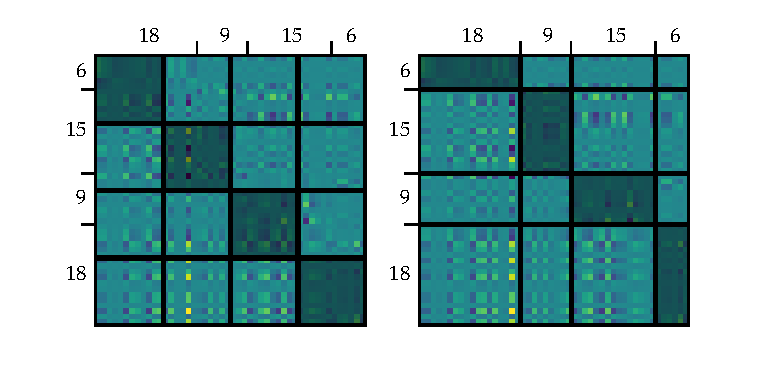
\includegraphics[trim=0.4cm 0.9cm 0 0, clip,width=\textwidth]{Plots/example_move.pdf}
	\begin{subfigure}[b]{0.35\textwidth}
		\caption{Initial system}
		\label{fig:example_move_a}
	\end{subfigure}
	\hspace{0.8cm}
	\begin{subfigure}[b]{0.35\textwidth}
		\caption{Optimized system}
		\label{fig:example_move_b}
	\end{subfigure}
	\caption{Illustration of the initial system and the optimized system.
		The lines mark the segmentation of the system.
		The matrices $D$ are shaded in gray.
		The ticks show the segmentation of the matrix $A$. 
		We can see that the segmentation of the optimized system coincides with the segmentation of $A$.}
	\label{fig:example_move}
\end{figure}
Now I represent the matrix with a time varying system without using the knowledge about the input and output dimensions.
For this I first create a system with constant input and output dimensions.
This system is illustrated in Figure\,\ref{fig:example_move_a}.
Then the segmentation is adapted using Algorithm\,\ref{alg:optimize segemtnation}.
As an objective function I used the normalized nuclear norm as described in Equation\,\ref{eq:objective_nuc}.
This gives the system illustrated in Figure\,\ref{fig:example_move_b}.
We can see that the algorithm can recover the original segmentation.

When the algorithm adapts the segmentation, it tests different segmentation and uses the one with the lowest objective function.
This is done in every iteration. 
\begin{figure}[!htb]
	\centering
	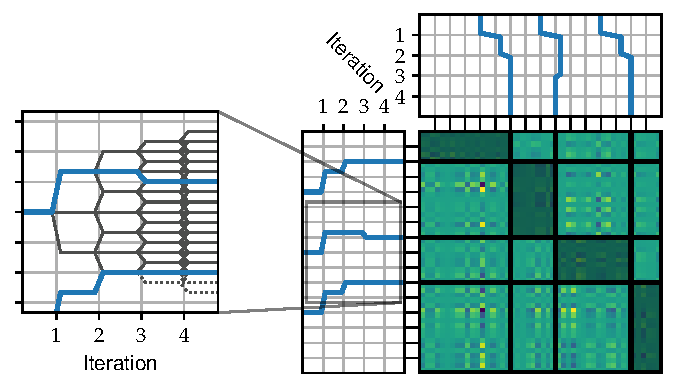
\includegraphics[width=0.87\textwidth]{Plots/example_move_iterations.pdf}
	\begin{subfigure}[b]{0.3\textwidth}
		\caption{Illustration of all possible search paths}
		\label{fig:example_move_bound_a}
	\end{subfigure}
	\begin{subfigure}[b]{0.55\textwidth}
		\caption{Illustration of the change of the segmentation}
		\label{fig:example_move_bound_b}
	\end{subfigure}
	\caption{Illustration of the change of the segmentation.
		The blue lines mark how the boundaries change as the algorithm adapts the segmentation.
	}
	\label{fig:example_move_bound}
\end{figure}
The search distance $l_i$ determines which movements of boundaries are tested at every iteration.
In the first iterations a larger $l_i$ is used. 
For the later iterations the $l_i$ are smaller.
I used $l = [4,2,1,1]$ as search distances for this example.
The Plot in Figure\,\ref{fig:example_move_bound_a} shows all the positions that are possible at every iteration.
We can see that in the first iterations the possible changes are larger and decrease for further iterations.
We can also observe that it is possible to reach the same segmentation using different paths.
The algorithm also makes sure, that the boundaries do not cross.
Therefore, some paths are not possible as these would require crossing another boundary. 
In Figure\,\ref{fig:example_move_a} these are drawn with dotted lines.
The Figure\,\ref{fig:example_move_bound_b} shows how the segmentation is changing between the iterations. 

%The algorithm does not always converge to the original segmentation if the Hankel matricies have a higher rank.

\subsection{Weight Matrix Approximation}
Now the algorithm is tested for weight matrices.


\paragraph{Mobilenet V2}
First a weight matrix $M$ from the \emph{Mobilenet V2} model is used.
The size of the matrix is ${1000 \times 1280}$.
I set the number of stages to $K = 10$ based on the approximations done in Section\,\ref{sec:Choose_K}.
In Section\,\ref{sec:Choose_K} the input and output dimensions are presumed to be constant.
Because this is not the case for the tested matrix, I also tested other $K$s.
As the objective function I use the number of multiplications as defined in Equation\,\ref{eq:objective_flop}.
I chose $\epsilon = \frac{1}{4} \|M\|_H$ as the threshold value for which the segmentation is optimized.
The value of $\|M\|_H$ is calculated using the initial segmentation.
I use the search sequence $l = [30, 20, 14,  9,  6,  4,  3,  2,  2,  1]$.
This search sequence also starts with lager search distances, that decrease over time.

\begin{figure}[!htb]
	%\centering
	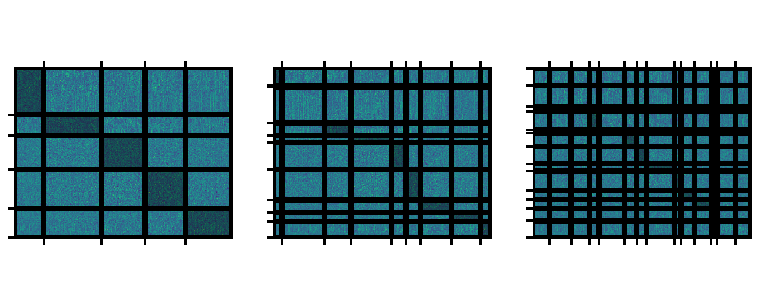
\includegraphics[trim=0.4cm 0.9cm 0 0, clip,width=\textwidth]{Plots/Mobilenet_diff_K.pdf}
	\begin{subfigure}[b]{0.3\textwidth}
		\caption{$K=5$  $\f_{\text{FLOP}}=561549$}
	\end{subfigure}
	\begin{subfigure}[b]{0.34\textwidth}
		\caption{$K=10$  $\f_{\text{FLOP}}=480573$}
	\end{subfigure}
	\begin{subfigure}[b]{0.34\textwidth}
		\caption{$K=17$ $\f_{\text{FLOP}}=494119$}
	\end{subfigure}
	\caption{Matrix segmentation for different numbers of Stages.
		The areas shaded in gray represent the $D$-matrices.
		For higher numbers of stages the portion represented by the $D_k$-Matrices gets lower.}
	\label{fig:Mobilenet_diff_Ks}
\end{figure}
The results for $K=5$, $K=10$ and $K =17$ are illustrated in Figure\,\ref{fig:Mobilenet_diff_Ks}.
The different numbers of stages result in different numbers of multiplications.
For $K=10$ I get the lowest number of multiplications.
%First I try $\f_{\text{nuc}}(\Sigma)$ as defined in Equation\,\ref{eq:objective_nuc} as objective function.
%As search sequence I use $l = [120,  80,  54,  36,  24,  16,  11,   8,   5,   4]$
%The result is illustrated in Figure\,\ref{fig:mobilenet_seperation_nuc}.
%We can see that the boundaries do not converge. 
%The boundaries keep moving towards the edges of the matrix.
%This results in a large $D$-Matrices.
%\begin{figure}[!htb]
%	\centering
%	\includegraphics[width=0.682\textwidth]{Plots/move_example_mobilenet_nuc.pdf}
%	\caption{Illustration of the change of the segmentation with Nuclear norm optimization.
%		Note the large shaded areas that represent the $D$-matrices.
%	}
%	\label{fig:mobilenet_seperation_nuc}
%\end{figure}
%Therefore $\f_{\text{nuc}}(\Sigma)$ is not a suitable objective function.
The change of the segmentation for $K=10$ is illustrated in Figure\,\ref{fig:mobilenet_seperation_comp}.
\begin{figure}[!htb]
	\centering
	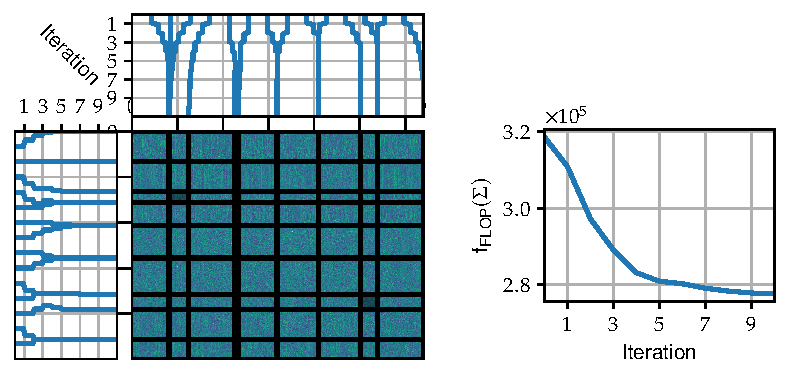
\includegraphics[width=0.93\textwidth]{Plots/move_example_mobilenet_comp.pdf}
	\caption{Illustration of the change of the segmentation for the weight matrix from \emph{Mobilenet V2} model.
	}
	\label{fig:mobilenet_seperation_comp}
\end{figure}
%On the right the objective function $f_\text{FLOP}(\Sigma)$ is plotted.
We can see that the number of operation decreases, as the algorithm runs, as plotted on the right of Figure\,\ref{fig:mobilenet_seperation_comp}.
Note that some input and output dimensions vanish. 
In Figure\,\ref{fig:mobilenet_seperation_comp} this shows as bounds converging to the same point. This also leads to the effect that only a small part of the matrix is represented with the $D_k$-matrices.
\begin{figure}[!htb]
	\centering
	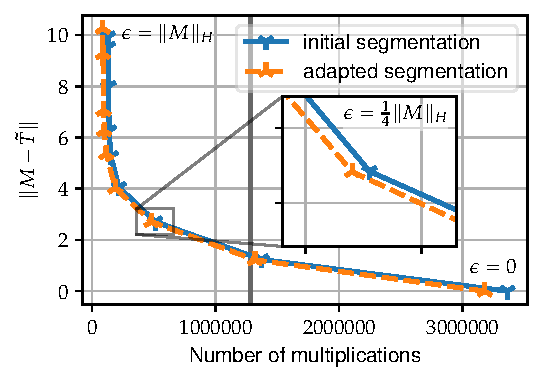
\includegraphics[width=0.7\textwidth]{Plots/move_example_mobilenet_error.pdf}
	\caption{Plot of the approximation error with respect to the number of multiplications for different $\epsilon$. 
		The black line indicates the number of multiplications for the regular matrix vector product. 
	}
	\label{fig:mobilenet_err_cost}
\end{figure}
The resulting system requires more multiplications to compute $y=Tu$ as required for a regular matrix vector multiplication.
Therefor the system complexity is reduced using balanced truncation as described in Section\,\ref{sec:approx}.
This is done for evenly spaced approximation parameters $\epsilon$ in the range form 0 to $\|M\|_H$.
For every $\epsilon$ the number of multiplications and the approximation error $\| M-\tilde{T} \|$ are computed and plotted in Figure\,\ref{fig:mobilenet_err_cost}.
The results for the original and the adapted segmentation is shown.
%We can see that the adaptation of the segmentation does not yield big changes.
For the case $\epsilon = \frac{1}{4} \|M\|_H$ we can see that the number of multiplications 
did decrease by $6\%$ as shown in Figure\,\ref{fig:mobilenet_seperation_comp}.
The approximation error $\| M-\tilde{T} \|$ did not change due to the adaption of the segmentation.

The state dimensions of the initial and adapted systems are plotted in Figure\,\ref{fig:mobilenet_state_dims_move}.
One can see that while some state dimensions decreased others did not decrease or even increased significantly.
In total, the number of states decreased.
\begin{figure}[!htb]
	\centering
	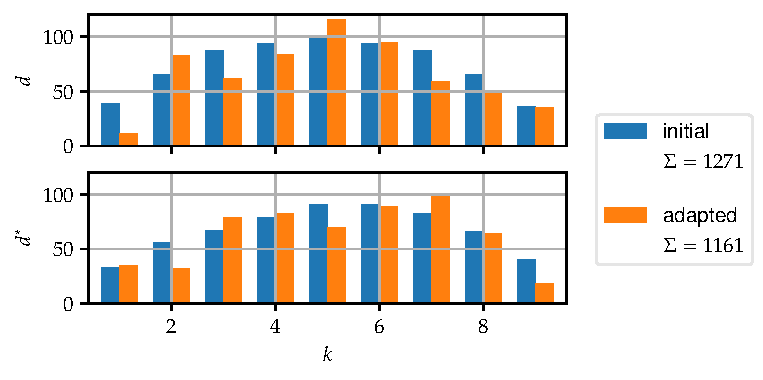
\includegraphics[width=\textwidth]{Plots/move_example_mobilenet_state_dims.pdf}
	\caption{Plot of the causal state dimensions $d_k$ and the anticausal state dimensions $d_k^*$ before and after the adaptation of the segmentation for $\epsilon = \frac{1}{4} \|M\|_H$
	}
	\label{fig:mobilenet_state_dims_move}
\end{figure}

\paragraph{AlexNet}
Now a weight matrix $M$ form the \emph{AlexNet} model with the size ${4096 \times 9216}$ is represented.
For this matrix I use $K=15$, using the approximation described in Section\,\ref{sec:Choose_K}.
As the matrix is wide, I use different search distances for the inputs and outputs.
For the output I use the search distances $l =  [120,  86,  62,  44,  32,  23,  16,  12,   9,   6]$.
And for the input $l =  [270, 193, 138,  99,  71,  51,  36,  26,  19,  14]$.
Here the threshold value is again $\epsilon = \frac{1}{4} \|M\|_H$, based on the initial segmentation.
To speed up the computation, the system is approximated with balanced truncation before the segmentation is adapted.
This is done using the threshold $\epsilon_{\text{apr}}=\frac{1}{2} \epsilon$.
It is important to choose an smaller $\epsilon$ for the approximation than for the adaptation.

\begin{figure}[!htb]
	\centering
	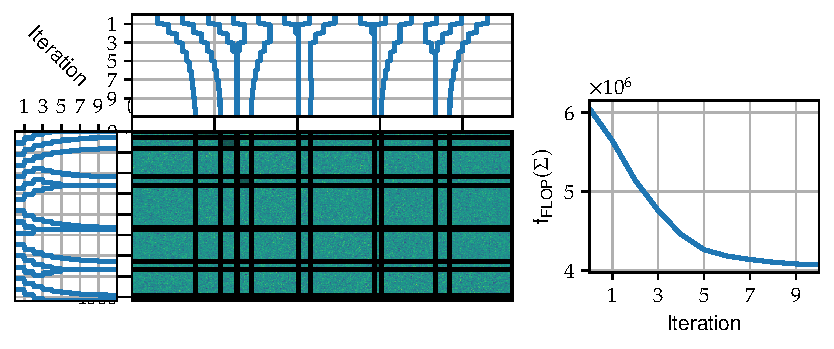
\includegraphics[width=\textwidth]{Plots/move_example_alexnet_comp.pdf}
	\caption{Illustration of the change of the segmentation for the weight matrix from \emph{AlexNet} model.
	}
	\label{fig:alexnet_seperation_comp}
\end{figure}
Then I adapted the segmentation using Algorithm\,\ref{alg:optimize segemtnation}.
The systems are again approximated using balanced truncation.
After moving the bounds the number of multiplications for $\epsilon = \frac{1}{4}\|M\|_\text{H}$ is reduced by \todo{calc when redoing plots}.
As the adaptation of the segmentation was not performed on the full system, but only on an approximated system, adaptation errors can be amplified.
\begin{figure}[!htb]
	\centering
	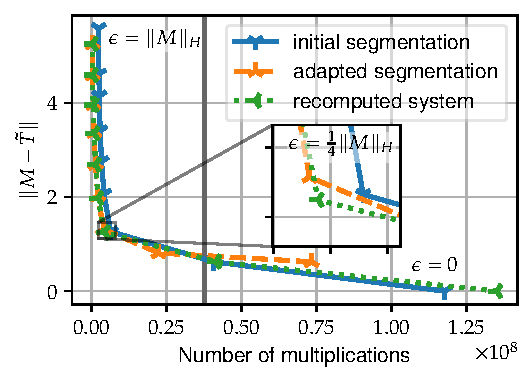
\includegraphics[width=0.7\textwidth]{Plots/move_example_alexnet_error.pdf}
	\caption{Plot of the approximation error with respect to the number of multiplications for different $\epsilon$. 
		The black line indicates the number of multiplications for the regular matrix vector product. 
		TODO: recomputed,add eps,readability
	}
	\label{fig:allexnet_err_cost}
\end{figure}
We can see in Figure\,\ref{fig:alexnet_seperation_comp} that the approximation error actually increased after applying the Algorithm\,\ref{alg:optimize segemtnation}.
We can also observe that the approximation error for the adapted system does not vanish for an balanced truncation with $\epsilon = 0$ as the system is based on an already approximated system.
Therefore, a new system is computed. 
This system has the same input and output dimensions as the adapted system but is directly calculated form the matrix $M$.
This system is subsequent approximated using balanced truncation.
The recomputed system with the new borders has the lowest approximation error.
The number of multiplications increases slightly for the recomputed system compared to the adapted system.
The number of multiplication is still $31\%$ less compared with the initial system for $\epsilon = \frac{1}{4}\|M\|_\text{H}$.
For smaller $\epsilon$s,  the recomputed system behaves similar to the initial system.


%The number with the new segmentation is lower than for initial segmentation if $\epsilon \geq \frac{1}{4} \|A\|_H$.
%The reidentified system has requires an equal or higher number of multiplications if $\epsilon < \frac{1}{4} \|A\|_H$.
%This is due to the fact that in this case the necessary information has been removed before the running Algorithm\,\ref{alg:optimize segemtnation}.

\section{Permutations}\label{sec:test_perm}
In this section the algorithm described in Section\,\ref{sec:permutation} is tested.
Here an initial system with one stage is created.
The stage is than spit up in two stages.
This process is then repeated.
When the stages are split, the inputs and outputs are partitioned such that a objective function is minimized.
This makes it possible to recover a permuted sequentially semiseparable matrix.

\subsection{Illustrative example}
First the algorithm is tested on a random sequential semiseparable matrix $T$.
The Hankel matrices have rank $2$.
The matrix is generated as described in Appendix\,\ref{A:random_T}. 
The rows and columns of the matrix are then permuted with random permutations.
Then Algorithm\,\ref{alg:split} is used to identify the system.
The result is shown in Figure\,\ref{fig:example_permute}.
\begin{figure}[!htb]
	\centering
	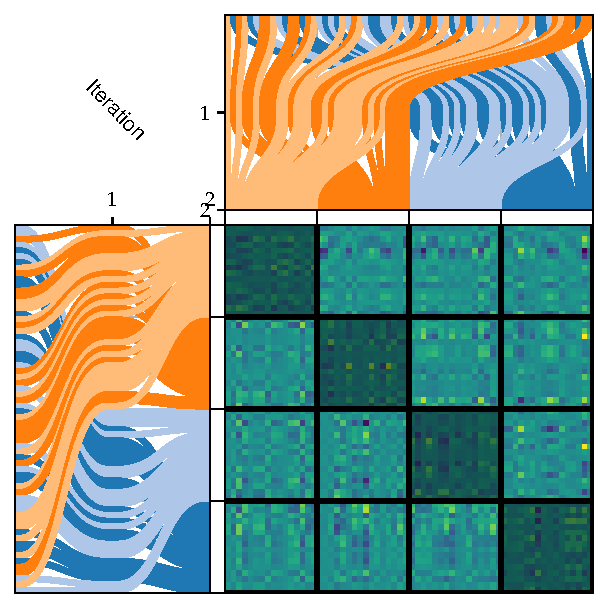
\includegraphics[width=0.65\textwidth]{Plots/example_permute.pdf}
	\caption{Illustration of the permuted sequentially matrix.
		The connections at the top and the left illustrate how the original segmentation is recovered by permuting the input and output.
		This is done in two iterations of the algorithm.
	}
	\label{fig:example_permute}
\end{figure}
During the first iteration the algorithm splits the initial stage into two stages
We can see how the algorithm partitions the inputs and outputs in two groups and reorders them accordingly.
After this, the stages are again split into four stages total.
In the second iteration the inputs and outputs of each stage are then again grouped into two subgroups each and ordered accordingly.
The algorithm is able to recover the permutation.

\subsection{Weight Matrix Approximation}
The algorithm is tested on weight matrices.
These have the property that the Hankel matrices usually have close to full rank. 
As algorithm to minimize the rank does usually increase the computational cost in this case, the Frobenius norm of the Hankel matrices is used as objective function.
\paragraph{Mobilenet V2}
Next the algorithm is used to represent a weight matrix from the \emph{Mobilenet V2} model.
Here the inputs and outputs are partitioned such that the Forbenius norm of the Hankel matrices is minimized.
As the algorithm can only use numbers of stages that are powers of $2$, I use $K=2^3=8$ as it is closest to $K=10$.
The regularization parameter is set to $\gamma=9\times10^5$.
This makes sure that the inputs and outputs are divided into two nearly equally sized parts.
The resulting permuted matrix is shown in Figure\,\ref{fig:mobilenet_permutation}.
\begin{figure}[!htb]
	\centering
	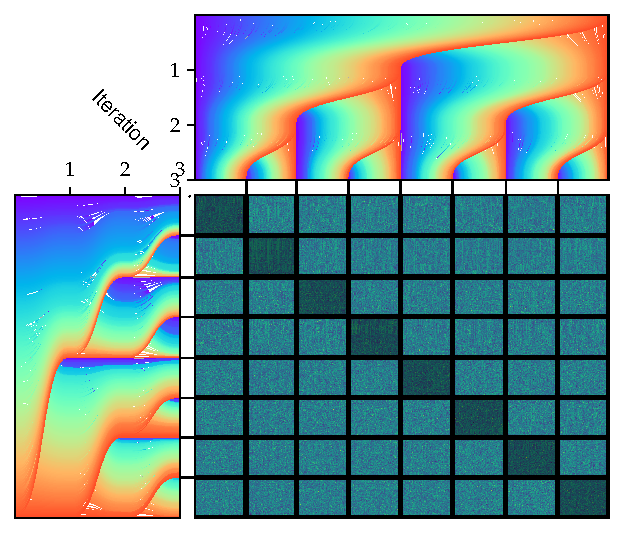
\includegraphics[width=0.9\textwidth]{Plots/Mobilenet_permute.pdf}
	\caption{Illustration of permuted weight matrix from \emph{Mobilenet V2} model.
	}
	\label{fig:mobilenet_permutation}
\end{figure}
As a reference, a system without permutations is computed.
The reference system and the permuted system are approximated using balanced truncation.
We can see in Figure\,\ref{fig:mobilenet_err_cost_perm} that permuting the matrix has only a minor impact on the number of operations and the approximation error.
For $\epsilon = \frac{1}{4}\|M\|_\text{H}$ the reduction of the computational cost due to the permutation is $<1\%$.

\begin{figure}[!htb]
	\centering
	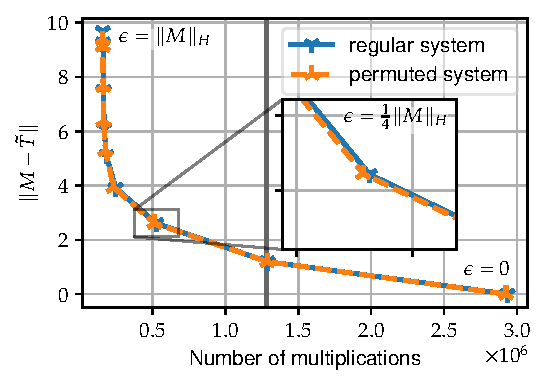
\includegraphics[width=0.7\textwidth]{Plots/perm_example_mobilenet_error.pdf}
	\caption{Plot of the approximation error with respect to the number of multiplications for different $\epsilon$. 
		The black line indicates the number of multiplications for the regular matrix vector product. 
		TODO: regular,add eps,readability
	}
	\label{fig:mobilenet_err_cost_perm}
\end{figure}

The state dimensions of the regular and permuted systems are plotted in Figure\,\ref{fig:mobilenet_state_dims_perm}.
One can see that while most state dimensions decreased others did increase.
In total, the number of states did only slightly decrease.
This means that the algorithm is only partially successful in decreasing the number of states.
\begin{figure}[!htb]
	\centering
	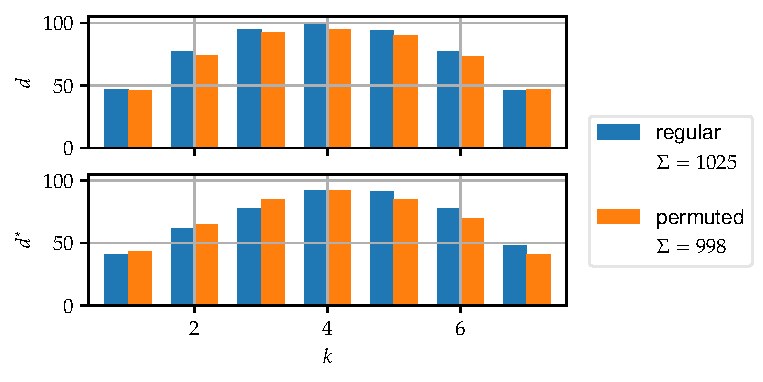
\includegraphics[width=0.93\textwidth]{Plots/perm_example_mobilenet_state_dims.pdf}
	\caption{Plot of the causal state dimensions $d_k$ and the anticausal state dimensions $d_k^*$ for the regular and permuted system for $\epsilon = \frac{1}{4} \|M\|_H$
	}
	\label{fig:mobilenet_state_dims_perm}
\end{figure}

\paragraph{Alexnet}
The algorithm returns similar results for the weight matrix form the \emph{AlexNet} model.
For this the $K = 2^4 = 16$ was used and $\gamma =  6\times10^3$.
The number of flops is reduced by $3\%$ if the system is approximated with $\epsilon = \frac{1}{4}\|M\|_\text{H}$.




\chapter{Discussion}\label{chap:discussion}
The two algorithms presented in this thesis were able to recover the structure of simple test cases based on random sequentially matrices.
When applied to the tested weight matrices, they were not able to identify a potential structure in the weight matrices.

Regardless, optimizing the segmentation for the computational cost did lead to a noticeable reduction of the computational cost as seen in Section\,\ref{sec:test_adao}.
The total number of states decreased, even if some state dimension got larger. 
This reduction of the computational cost is possible without a significant worsening of the approximation error. 
As the algorithm can also run on an pre-approximated system, the segmentation of relatively large matrices like the \emph{Alexnet} weight matrix can be computed on an regular notebook.
One notable observation is that the size of the $D_k$ decrease.
In some cases, the inputs or outputs of stages are zero-dimensional.
It might be interesting to explore time varying systems that do not have $D_k$.
Alternatively, the $D_k$ could be represent using other matrix approximations like low rank approximations. 

The second approach based on recursive splitting, tested in Section\,\ref{sec:test_perm} did not return promising results.
Reducing the sum of the squared Hankel singular values did only lead to a very small reduction of the computational cost, as the number of states only minimally decreased.
This also suggests that the potential for decreasing the computational cost for system representations of weight matrices by reducing the number of states is limited.
Focusing directly on the computational cost seems to be a better approach.

I was not able to identify sequentially semiseparable structures in the weight matrices using a simple adaptation of the segmentation.
This is also not surprising, as this would require that the Hankel matrices of the weight matrices have low rank, but this was not experienced in any experiment.
It might be possible to find structures when allowing for permutations as this has more degrees of freedom. 
Unfortunately, the splitting algorithm based on the minimization of the Forbenius nor was not able to do this.
Here an optimization based on the nuclear norm, that promotes low rank solutions might be preferable, even if this would require some improvements to make the optimization problem computationally viable.
The fact that the Hankel matrices of the weight matrices is consistent with other research.
%Different strategy for clustering
%Approaches in this thesis can help to reduce computational cost.
%Not able to find sequentially semiseparable structures in weight matrices.

%Permutation not successful
%mainly changing the Segemntation not reducing the number of states.
%Vanishing  input and output dimensions. Also vanishing $D$-matrices
Research by Martin and Mahoney suggests that weight matrices usually have full rank \cite{martin_implicit_2021}.
This might be explained with information theory \cite{papyan_traces_2020}.
The full rank property is in principle no problem, as sequentially semiseparable matrices can have full rank, even if the Hankel matrices have low rank. 
\footnote{For a trivial example consider the identity matrix as sequentially semiseperabel matrix with full rank}
I was not able to find statements if these results also hold for submatrices.
Even if similar results hold true for submatrices, approximations using time varying systems might be still beneficial, if the bulk of the singular values is sufficiently small.
In this case the approximation error would be small, even if many nonzero singular values would have to be removed.



%4-5 4pages

\chapter{Conclusion}\label{chap:conclusion}
%1-2 pages
The goal of this thesis was to develop and test algorithms that can be used to approximate matrices using time varying systems.

I developed some algorithms to transform time varying systems.
These are also useful for other applications involving time varying systems.
%One important feature is the computation of the Hankel singular values.
An important result are the techniques to obtain the Hankel singular values without explicitly computing the Hankel matrices.
The Hankel singular values are important as they are needed to approximate a system with balanced truncation.
This allows an efficient approximation of arbitrary systems similar to the technique described in \cite{chandrasekaran_fast_2005}.
If a system has to be reduced to a minimal system using floating point arithmetic, then this also gives a good way to do this in a well-defined fashion.
The Algorithm to split stages stated in \cite{chandrasekaran_fast_2005} was extended such that it can compute the Hankel singular values.
This makes it possible to use the algorithm to identify and later refine systems and obtain the Hankel singular values on the fly.
Also, algorithms to change the input and output dimensions are devised. 
Such algorithms are required if systems with not compatible dimensions have to be added or multiplied.
The work on this thesis also lead to improvements in the \emph{tvsclib}-library \cite{kissel_time_2022}.

To devise the number of stages, the computational cost for computing the matrix vector product with a time varying system was estimated.
Using this estimation, it is possible to choose the number of stages for approximations.
This estimation might also serve as a baseline if one needs to determine how the structural parameters must be chosen to reduce the computational cost.
These are not only required if an existing matrix is approximated but also could be used as a baseline if a neural network based on a time varying system is trained from scratch.

These results where combined with optimization problems to approximate weight matrices form neural networks.
The algorithm to adapt the segmentation of the matrix is able to reduce the computational cost of the system, even if no clear structure is identified.
The second approach based on spiting the stages did only yield minor improvements.
Some ideas used for the spiting might be interesting for other matrix structures.
Especially in the case of $\mathcal{H}$-matrices.
These also rely on recursively splitting the matrix into submatrices.
When weight matrices are approximated with $\mathcal{H}$-matrices, this require nonstandard admissibility conditions to determine if a matrix can be represented using a low rank approximation.

The techniques to change the segmentation can be used without increasing the approximation error measured in the spectral norm.
In this thesis I did not test how this influences the total accuracy of the neural network. 
The approximation error does give an indication but does not fully describe the behavior.
Future research is needed to determine how the approximation and the changing of the segmentation influences the accuracy of the neural network.
\todo[inline]{maybes something more optimistic}

\appendix
\chapter{Matrix Approximation Error Bounds}\label{A:Error Bounds}

In this chapter a proof for the Equation\,\ref{eq:error_spectral}
\begin{equation}
\|T-\hat{T}\| \leq \sum_{i=1}^K \|T-\hat{T}^{(k)}\| .
\end{equation}
and for the Equation\,\ref{eq:error_spectral}
\begin{equation}
\|T-\hat{T}\|_\text{F} \leq \sum_{i=1}^K \|T-\hat{T}^{(k)}\|_\text{F}
\end{equation}
is given.
To prove the bound we decompose the change due to the balanced truncation into
\begin{equation}\label{eq:decomposition_approx_sum}
	T-\hat{T} =
	\begin{bmatrix}
	&\Delta_0^*\\
	\breve{\Delta}_1
	\end{bmatrix}
	+
	\begin{bmatrix}
	&\breve{\Delta}_1^*\\
	\breve{\Delta}_2
	\end{bmatrix}
	+\dots+
	\begin{bmatrix}
	&\breve{\Delta}_{K-1}^*\\
	\Delta_K
	\end{bmatrix}
	.
\end{equation}
The matrix $\Delta_k$ denotes the difference caused by the balanced truncation of the state $k$ on the original system
\begin{equation}
	\Delta_k = \Ob_{k}\R_{k} - \hat{\Ob}_k\hat{\R}_k = \Ob_{k[2]}\R_{k[2]}
\end{equation}
and the matrix $\breve{\Delta}_k$ denotes the difference causes by a balanced truncation of the state $k$ if the later stages have already been truncated using balanced truncation. 
For the causal system this can be expressed as 
\begin{equation*}
\tilde{\Delta}_k=
	\begin{bmatrix}
	C_k\\
	\hat{\Ob}_{k+1}\begin{bmatrix}
	A_{k+1[11]}&A_{k+1[12]}
	\end{bmatrix}
	\end{bmatrix}
	R_k
	-
	\begin{bmatrix}
C_k\\
\hat{\Ob}_{k+1}
A_{k+1[11]}
\end{bmatrix}
R_{k[1]}
= 
\begin{bmatrix}
C_{k[2]}\\
\hat{\Ob}_{k+1}A_{k+1[12]}
\end{bmatrix}
R_{k[2]}
\end{equation*}
Here the matrix $\hat{\Ob}_{k+1}$ denotes the observability matrix of the approximated system 
\begin{equation}
\hat{\Ob}_{k+1}=
\begin{bmatrix}
\hat{C}_{k+1}\\
\hat{C}_{k+2}\hat{A}_{k+1}\\
\vdots \\
\hat{C}_{K} \hat{A}_{K-1} \dots \hat{A}_{k+1}
\end{bmatrix}
=
\begin{bmatrix}
C_{k+1[1]}\\
C_{k+2[1]}A_{k+1[11]}\\
\vdots\\
C_{K[1]}A_{K-1[11]}\dots A_{k+1[11]}
\end{bmatrix}
\end{equation}

Using the triangle inequality we obtain the relation
\begin{equation}
\|T-\hat{T}\| \leq
\Bigg\|
\begin{bmatrix}
&\Delta_0^*\\
\breve{\Delta}_1
\end{bmatrix}
\Bigg\|+\Bigg\|
\begin{bmatrix}
&\breve{\Delta}_1^*\\
\breve{\Delta}_2
\end{bmatrix}
\Bigg\|+\dots+\Bigg\|
\begin{bmatrix}
&\breve{\Delta}_{K-1}\\
\Delta_K
\end{bmatrix}
\Bigg\|.
\end{equation}

\paragraph{Spectral Norm}
The idea is to prove that $\|\Delta_k\|$ is equal or larger than the actual introduced difference $\|\breve{\Delta}_k\|$.
Using the bound form Equation\,\ref{eq:bound_single} we can then bound the matrix
\begin{equation}
\Bigg\|
\begin{bmatrix}
& \breve{\Delta}_{k-1}^*\\
\breve{\Delta}_k
\end{bmatrix}
\Bigg\| \leq \max{\sigma}
\end{equation}

To prove $\|\breve{\Delta}_k\| \leq \|\Delta_k\|$ it is sufficient to prove
\begin{equation}\label{eq:A_breve_leq_delta}
	\|\breve{\Delta}_k u\|_2 \leq \|\Delta_k u\|_2 
\end{equation}
for any vector $u$.
\begin{proof}
	For this we use the definition of the spectral norm
	\begin{equation}
		\|\breve{\Delta}_k\| =
		\underset{\|u\|_2 = 1}{\max}(\|\breve{\Delta}_k u\|_2)
		\leq 
		\underset{\|u\|_2 = 1}{\max}(\|\Delta_k u\|_2)
		=\|\Delta_k\|
	\end{equation}
\end{proof}

For the causal case we start with the equation
\begin{equation}
	\|\Delta_k u\|_2^2 = \|\Ob_{k[2]}] \R_{k[2]} u\|_2^2
\end{equation}
By inserting the definitions form Equation\,\ref{eq:reduced_system} and using the factorization from Equation\,\ref{eq:decomp_O} we obtain 
\begin{equation}
	\Bigg\|
	\begin{bmatrix}
	\eye & \\
	& \Ob_{K+1}
	\end{bmatrix}
	\begin{bmatrix}
	C_{k[2]}\\
	\begin{bmatrix}
	A_{k[12]}\\
	A_{k[22]}
	\end{bmatrix}
	\end{bmatrix}  \R_{k[2]} u\Bigg\|_2^2
\end{equation}
Now we use balanced truncation of the state $x_{k+1}$.
This analogous splits up the observability matrix $\Ob_{k+1}$ according to
\begin{equation}
	\Ob_{k+1} = 
	\begin{bmatrix}
	\Ob_{k+1[1]} & \Ob_{k+1[2]}
	\end{bmatrix}
\end{equation}
Using this $\|\Delta_k u\|_2^2$ can be expressed as
\begin{equation}
	\Bigg\|
\begin{bmatrix}
C_{k[2]}\\
\Ob_{k+1[1]}A_{k[12]}+
\Ob_{k+1[2]}A_{k[22]}
\end{bmatrix}  \R_{k[2]} u\Bigg\|_2^2
.
\end{equation}
Using the properties of the balanced realization the norm can be split up in the sum
\begin{equation}
\Big\|
\begin{bmatrix}
C_{k[2]}\\
\Ob_{k+1[1]}A_{k[12]}
\end{bmatrix}  \R_{k[2]} u
\Big\|_2^2
+
\Big\|
\Ob_{k+1[2]}A_{k[22]}
 \R_{k[2]} u
\Big\|_2^2
.
\end{equation}
\begin{proof}
%	\begin{align}
%		&\Bigg\|
%		\begin{bmatrix}
%		C_{k[2]}\\
%		\Ob_{k+1[1]}A_{k[11]}+\Ob_{k+1[2]}A_{k[21]}
%		\end{bmatrix}  \R_{k[2]} u
%		\Bigg\|_2^2\\
%		&=
%		u^\top \R_{k[2]}^\top
%		\begin{bmatrix}
%C_{k[2]}^\top &
%\Ob_{k+1[1]}A_{k[11]}^\top+\Ob_{k+1[2]}A_{k[21]}^\top
%\end{bmatrix}  
%		\begin{bmatrix}
%C_{k[2]}\\
%\Ob_{k+1[1]}A_{k[11]}+\Ob_{k+1[2]}A_{k[21]}
%\end{bmatrix}  \R_{k[2]} u		
%	\end{align}
\begin{align}
		&\Bigg\|
	\begin{bmatrix}
	\eye & \\
	& \Ob_{K+1}
	\end{bmatrix}
	\begin{bmatrix}
	C_{k[2]}\\
	\begin{bmatrix}
	A_{k[12]}\\
	A_{k[22]}
	\end{bmatrix}
	\end{bmatrix}  \R_{k[2]} u\Bigg\|_2^2
	\\
	&=
	u^\top
	\R_{k[2]}^\top
	\begin{bmatrix}
	C_{k[2]}^\top&
	\begin{bmatrix}
	A_{k[12]}^\top&
	A_{k[22]}^\top
	\end{bmatrix}
	\end{bmatrix} 
	\begin{bmatrix}
	\eye & \\
	& \Ob_{K+1}^\top
	\end{bmatrix} 
	\begin{bmatrix}
	\eye & \\
	& \Ob_{K+1}
	\end{bmatrix}
	\begin{bmatrix}
	C_{k[2]}\\
	\begin{bmatrix}
	A_{k[12]}\\
	A_{k[22]}
	\end{bmatrix}
	\end{bmatrix}  
	\R_{k[2]} u
\end{align}
using the fact that the system is balanced and therefore $\Ob_{k+1}^\top \Ob_{k+1} = \Sigma_{k+1}$
\begin{equation}
u^\top
\R_{k[2]}^\top
\begin{bmatrix}
C_{k[2]}^\top&
\begin{bmatrix}
A_{k[12]}^\top&
A_{k[22]}^\top
\end{bmatrix}
\end{bmatrix} 
\begin{bmatrix}
\eye & \\
& \Sigma_{K+1}
\end{bmatrix} 
\begin{bmatrix}
C_{k[2]}\\
\begin{bmatrix}
A_{k[12]}\\
A_{k[22]}
\end{bmatrix}
\end{bmatrix}  
\R_{k[2]} u
\end{equation}
By splitting $\Sigma_{k+1}$ with the appropriate dimensions such that  $\Sigma_{k+1} = \diag(\Sigma_{k+1[1]},\Sigma_{k+1[2]})$ we can rewrite the expression as
\begin{equation}
u^\top
\R_{k[2]}^\top
\begin{bmatrix}
C_{k[2]}^\top&
A_{k[12]}^\top&
A_{k[22]}^\top
\end{bmatrix} 
\begin{bmatrix}
\eye & \\
& \Sigma_{K+1[1]}\\
& & \Sigma_{K+1[2]}
\end{bmatrix} 
\begin{bmatrix}
C_{k[2]}\\
A_{k[12]}\\
A_{k[22]}
\end{bmatrix}  
\R_{k[2]} u
.
\end{equation}
This allows us to regroup the expression as the sum
\begin{align}
	&=
	u^\top
	\R_{k[2]}^\top
	\begin{bmatrix}
	C_{k[2]}^\top&
	A_{k[12]}^\top&
	\end{bmatrix} 
	\begin{bmatrix}
	\eye & \\
	& \Sigma_{K+1[1]}\\
	\end{bmatrix} 
	\begin{bmatrix}
	C_{k[2]}\\
	A_{k[12]}\\
	\end{bmatrix}  
	\R_{k[2]} u
\\&\quad\quad+
	u^\top
	\R_{k[2]}^\top
	A_{k[22]}^\top 
	\Sigma_{K+1[2]}
	A_{k[22]} 
	\R_{k[2]} u
	.
\end{align}
	It is also possible to prove this using the fact that $\range(\Ob_{k+1[1]})\perp \range(\Ob_{k+1[2]})$ and then employing $(u+v)^\top (u+v) = u^\top u + v^\top v$ for $u \perp v$
\end{proof}

Now we again use Equation\,\ref{eq:decomp_O} to rewrite the first summand as 
\begin{equation}
\Big\|
\begin{bmatrix}
C_{k[2]}\\
\Ob_{k+1[1]}A_{k[12]}
\end{bmatrix}  \R_{k[2]} u
\Big\|_2^2
=
\Big\|
\begin{bmatrix}
\eye\\&\eye\\&&\Ob_{k+2}
\end{bmatrix}
\begin{bmatrix}
C_{k[2]}\\
C_{k+1[1]}A_{k[12]}\\
\begin{bmatrix}
A_{k+1[11]}\\
A_{k+1[21]}
\end{bmatrix}
A_{k[12]}
\end{bmatrix}  \R_{k[2]} u
\Big\|_2^2
\end{equation}
Analogously we can spit the norm up again into the sum
\begin{align}
&=\Bigg\|
\begin{bmatrix}
\eye\\&\eye\\&&\Ob_{k+2}
\end{bmatrix}
\begin{bmatrix}
C_{k[2]}\\
C_{k+1[1]}A_{k[12]}\\
\begin{bmatrix}
A_{k+2[11]}\\
A_{k+2[21]}
\end{bmatrix}
A_{k[12]}
\end{bmatrix}  \R_{k[2]} u
\Bigg\|_2^2
\\
&=
\Bigg\|
\begin{bmatrix}
C_{k[2]}\\
C_{k+1[1]}A_{k[12]}\\
\Ob_{k+2[1]}A_{k+2[11]}A_{k[12]}+
\Ob_{k+2[2]}A_{k+2[21]}A_{k[12]}
\end{bmatrix}  \R_{k[2]} u
\Bigg\|_2^2
\\
&=
\Bigg\|
\begin{bmatrix}
C_{k[2]}\\
C_{k+1[1]}A_{k[12]}\\
\Ob_{k+2[1]}A_{k+2[11]}A_{k[12]}+
\end{bmatrix}  \R_{k[2]} u
\Bigg\|_2^2
+
\Big\|
\Ob_{k+2[2]}A_{k+2[21]}A_{k[12]}
\R_{k[2]} u
\Big\|_2^2
\end{align}
This can be repeated until we reach the final state $K$.
The remaining term is 
\begin{equation}
	\Bigg\|
	\begin{bmatrix}
	C_{k[2]}\\
	C_{k+1[1]}A_{k[12]}\\
	C_{k+2[1]}A_{k+1[11]}A_{k[12]}\\
	\vdots\\
	C_{K[1]}A_{K-1[11]}\cdots  A_{k+1[11]} A_{k[12]}
	\end{bmatrix}  \R_{k[2]} u
	\Bigg\|_2^2
	.
\end{equation}
The remaining term can be identified as 
\begin{equation}
\Bigg\|
\begin{bmatrix}
C_{k[2]}\\
\hat{\Ob}_{k+1}A_{k[12]}
\end{bmatrix}  \R_{k[2]} u
\Bigg\|_2^2
=
\Big\|\breve{\Delta}_k u\Big\|_2^2
.
\end{equation}
This allows us to decompose $\|\Delta_k u\|_2^2$ into the sum
\begin{equation}
\|\Delta_k u\|_2^2
	  =
	    \|\breve{\Delta}_k u\|_2^2
	  + \dots + \Big\|
	  \Ob_{k+1[2]}A_{k[21]}
	  \R_{k[2]} u
	  \Big\|_2^2
\end{equation}
Be reordering and using the fact that the squared norms larger or equal than $0$ we obtain the relation
\begin{equation}
	\|\breve{\Delta}_k u\|_2 \leq \|\Delta_k u\|_2 
	.
\end{equation}
This proves the relation form Equation\,\ref{eq:A_breve_leq_delta} for the causal matrices.
The anticausal case can be proven by transposing the matrix.
In this case the state $1$ is approximated first as indicated in Equation\,\ref{eq:decomposition_approx_sum}
The details are left as an exercise to the examiner.

\paragraph{Frobenius Norm}
Using Equation\,\ref{eq:A_breve_leq_delta} it is also straightforward to prove the relation for the Frobenius norm
as 
\begin{equation}
	\|M\|_\text{F}^2 = \trace(M^\top M) = \sum_{i=1}^{N} e_i^\top M^\top M e_i = \sum_{i=1}^{N} \|M e_i\|_2^2
\end{equation}
where $e_i$ is the $i$-th standard basis vector.
The relation $\|\breve{\Delta}_k e_i\|_2^2 \leq \|\Delta_k e_i\|_2^2$ implies that 
\begin{equation}
	\|\breve{\Delta}_k\|_\text{F} \leq \|\Delta_k\|_\text{F}
\end{equation}
\begin{equation}
\|T-\hat{T}\|_\text{F} \leq
\Bigg\|
\begin{bmatrix}
&\Delta_0^*\\
\breve{\Delta}_1
\end{bmatrix}
\Bigg\|_\text{F}+\Bigg\|
\begin{bmatrix}
&\breve{\Delta}_1^*\\
\breve{\Delta}_2
\end{bmatrix}
\Bigg\|_\text{F}+\dots+\Bigg\|
\begin{bmatrix}
&\breve{\Delta}_{K-1}\\
\Delta_K
\end{bmatrix}
\Bigg\|_\text{F}.
\end{equation}


\chapter{Random Sequentially semiseparable matrices}\label{A:random_T}

%In this section the construction of the random sequentially semiseparable matrices are  
In this section the algorithm to construct the sequentially semiseparable matrices used in Chapter\,\ref{chap:experiments} is explained.
The matrices can be parameterized with the the input dimensions $m_k$, the output dimensions $p_k$ and the rank of the  Hankel matrices.
The generated matrices have the property, that the range of $C$, $D$ and $G$ are orthogonal to each other.
Also the range of $B^\top$, $D^\top$ and $G^\top$ are orthogonal.


To archive the orthogonality, random orthogonal matrices form the Haar distribution are used.
The matrices are generated by the algorithm described in \cite{mezzadri_how_2007}, that is available in \emph{SciPy}.
Here we denote the group of orthogonal matrices with $n$ dimensions as $O(n)$.

For every stage $i \in 1, \dots ,K$ the matrices 
\begin{align}
	\tilde{U}_k &=p_k U_k  & \text{with } U_k &\in O(p_k)\\
	\tilde{V}_k &=m_k V_k  & \text{with } V_k &\in O(m_k)
\end{align}
are generated.
The matrices are scaled with $p_k$ and $m_k$ respectively to make sure that 
\begin{equation}
	\frac{\|v\|_2}{\length(v)} = 1  
\end{equation}
for all columns of $\tilde{V}_k$ and $\tilde{U}_k$.
The random sequentially semipermeable matrix $T$ with Hankel matrices of rank $d$ is constructed form the block matrices 
\begin{equation}
	T_{[i,j]} = 
	\begin{cases}
	\tilde{U}_{i[:,d]} \tilde{V}_{j[:,d]}^\top & \text{if } i<j\\
	\tilde{U}_{i[d+1,2d]} \tilde{V}_{j[d+1,2d]}^\top & \text{if } i=j\\
	\tilde{U}_{i[2d+1,3d]} \tilde{V}_{j[2d+1,3d]}^\top & \text{if } i>j\\
	\end{cases}
\end{equation}
These are then combined according to 
\begin{equation}
	T = \begin{bmatrix}
	T_{[1,1]} & T_{[1,2]} & \dots & T_{[1,k]}\\
	T_{[2,1]} & T_{[2,2]} & \dots & T_{[2,k]}\\
	\vdots & \vdots & \ddots &\vdots\\
	T_{[K,1]} & T_{[K,2]} & \dots & T_{[K,K]}
	\end{bmatrix}
\end{equation}

\printbibliography{}

\end{document}
